% Final thing is style report, not article.
\documentclass[12pt,a4paper]{report}

\usepackage{algpseudocode}
\usepackage{color}
\usepackage{amsmath}
\usepackage{tikz}
\usepackage{tabularx}
\usepackage{rotating}
\usepackage{subfigure}
\usepackage{amssymb}
\usepackage{xspace}

\newbox\subfigbox             % Create a box to hold the subfigure.
\makeatletter
  \newenvironment{subfloat}% % Create the new environment.
    {\def\caption##1{\gdef\subcapsave{\relax##1}}%
     \let\subcapsave=\@empty % Save the subcaption text.
     \let\sf@oldlabel=\label
     \def\label##1{\xdef\sublabsave{\noexpand\label{##1}}}%
     \let\sublabsave\relax    % Save the label key.
     \setbox\subfigbox\hbox
       \bgroup}%              % Open the box...
      {\egroup                % ... close the box and call \subfigure.
     \let\label=\sf@oldlabel
     \subfigure[\subcapsave]{\box\subfigbox}}%
\makeatother

\usetikzlibrary{arrows,decorations.pathmorphing,decorations.markings,backgrounds,positioning,fit,petri,automata,shapes,petri}

\pgfdeclarelayer{bg}
\pgfsetlayers{bg,main}

% MGK recommends these formatting settings:

% for hard-bound final submission, use:
\setlength{\oddsidemargin}{4.6mm}     % 30 mm left margin - 1 in
% for soft-bound version and techreport, use instead:
%\setlength{\oddsidemargin}{-0.4mm}    % 25 mm left margin - 1 in
\setlength{\evensidemargin}{\oddsidemargin}
\setlength{\topmargin}{-5.4mm}        % 20 mm top margin - 1 in
\setlength{\textwidth}{160mm}         % 20/25 mm right margin
\setlength{\textheight}{247mm}        % 20 mm bottom margin
\setlength{\headheight}{5mm}
\setlength{\headsep}{5mm}
\setlength{\parindent}{0mm}
\setlength{\parskip}{\medskipamount}
\renewcommand\baselinestretch{1.2}
\renewcommand\topfraction{.9}
\renewcommand\textfraction{.1}
\renewcommand\floatpagefraction{.8}

\author{Steven Smith}
\title{SLI: Speculative Lock Insertion}
\begin{document}

\tikzset{CfgInstr/.style={rectangle,minimum size=6mm}}
\tikzset{TrueCfgInstr/.style={rectangle,minimum size=6mm,fill=blue!50}}
\tikzset{DupeCfgInstr/.style={rectangle,minimum size=6mm,fill=blue!10}}
\tikzset{NewCfgInstr/.style={rectangle,minimum size=6mm,fill=red!50}}
\tikzset{stateSideEffect/.style={rectangle,draw}}
\tikzset{stateIf/.style={ellipse,draw}}
\tikzset{stateTerminal/.style={ellipse,draw}}
\tikzset{flowChartState/.style={rectangle,draw}}
\tikzset{killEdge/.style={decorate,decoration={snake,segment length=1mm,post length=0.4mm}}}
\tikzset{swungEdge/.style={color=red}}
\tikzset{happensBeforeEdge/.style={dashed}}
\tikzset{ifTrue/.style={}}
\tikzset{ifFalse/.style={dotted}}
\newcommand{\draftonly}[1]{#1}
\newcommand{\editorial}[1]{\draftonly{\textcolor{red}{\footnote{\textcolor{red}{#1}}}}}
\newcommand{\smh}[1]{\draftonly{\textcolor{green}{\footnote{\textcolor{green}{#1}}}}}
\newcommand{\needCite}{\draftonly{\editorial{need cite}}}
\newcommand{\todo}[1]{\draftonly{\textcolor{red}{#1}}}
\newcommand{\StateMachine}{program slice }
\newcommand{\StateMachines}{program slices }
\newcommand{\STateMachine}{Program slice }
\newcommand{\STateMachines}{Program slices }
\newcommand{\CrashSummary}{crash summary }
\newcommand{\CrashSummaries}{crash summaries }
\newcommand{\happensBefore}{\leftarrowtail}
\newcommand{\controlEdge}[2]{Control(#1 \rightarrow #2)}

\newcommand{\concatDynTraces}{\oplus}
\newcommand{\interleaveDynTraces}{\otimes}
\newcommand{\survive}{\top}
\newcommand{\crash}{\bot}
\newcommand{\queue}[1]{\{#1\}}
\newcommand{\map}[1]{\{#1\}}
\newcommand{\mapIndex}[2]{#1[#2]}
\newcommand{\state}[1]{\textsc{#1}}
\newcommand{\implementation}{\textcolor{blue}{implementation}}
\newcommand{\technique}{\textcolor{blue}{technique}}
\newcommand{\Implementation}{\textcolor{blue}{Implementation}}
\newcommand{\Technique}{\textcolor{blue}{Technique}}

\maketitle
\tableofcontents

\chapter{Abstract}
Blah.

\todo{I really need to come up with a better name for this; SLI really
  doesn't have anything to do with anything any more.}

Major todo items:

\begin{itemize}
\item The alias analysis needs a good editing.
\item The unification simplification needs a good editing.
\item So does the frame pointer elimination section.
\item Canonicalisation needs an almost complete rewrite.
\item The section on placing VCs needs rewriting.
\item The section on mandatory concurrency needs rewriting.  Or I could
   just drop it.
\item The entire eval section needs a lot more work.
\item Related work is a bit of a mess.
\item Conclusions are missing.
\item Need to do something cunning about enforcing contradictory HB graphs.
\item Need to come up with a better story on timeouts in the enforcers.
\item Kill off the compiled enforcer bits completely.
\item Kill off DRS mode completely.
\item The section on generating fixes needs a good editing.
\end{itemize}


\chapter{Introduction}
\section{Motivation}
Concurrency bugs are becoming more common, don't always have source (abandonware, libraries), so need something which works on binaries

\section{Overview of approach}
\subsection{Pipeline}
Overview of the basic pipeline: find bugs with bug finding more, then instantiate them into an enforcement patch, then analyse the core dump/DRS log to better characterise the bug, and then instantiate a fix.

\subsection{Analysis technique}
Overview of basic analysis technique: building \StateMachines which approximate a fragment of the program and then doing the analysis on that.
Explain that \StateMachines are derived for some specific behaviour which is currently being investigated, and that the simplifications used depend on that.
Explain that the specification of the behaviour must be a simple boolean i.e. the interesting thing either happens or does not happen, but that's usually not an issue because the \StateMachines themselves are reasonably computationally powerful (although not Turing complete), so properties like ``X must never be greater than 5'' can be checked without needing to check properties of X.
Explain that \StateMachines are acyclic and finite, and hence executions are also finite; makes analysis much, much easier.
Explain that they can cross function boundaries and can include fragments from multiple program threads.
Explain that each \StateMachine corresponds to some possible point in the program execution (defined by a set of suffixes of stacks, such that at least one thread must match each of the suffixes), and that if you have a snapshot of the program in that state you can interpret the \StateMachine to predict whether the program is going to experience the behaviour which is being investigated.

This is probably a good place to give some examples and a very informal semantics; the full semantics will wait until later.

\section{Background}
All the bits you need to understand before reading the rest of the dissertation.
Fairly dumb summary of a little bit of related work.


\chapter{Deriving and manipulating \StateMachines}
\label{chapter:derive_manip}
\section{Description of \StateMachines}
\label{sect:derive:description}

\todo{There's a pretty reasonable argument that this should be in the
  introduction.}

The core data structure used by {\technique} is the \StateMachine.
These consist of two main components: a
\introduction{summary}\editorial{Need a less generic-sounding name.}
of part of the program, in a simple (non-Turing complete) analysis
language, and an annotated fragment of the program's
\introduction{control flow graph (CFG)}, showing how states in the
\backref{summary} map to instructions in the program.

\backref{Summaries} themselves are acyclic graphs of
\introduction{analysis states}, which can be thought of as roughly
corresponding to possible points in the program's execution.  The
states themselves fall into one of four classes:

\begin{description}
\item[\introduction{Choice states}] These states have two successors
  and decide between them based on a condition, expressed as a
  \backref{BBDD}.  These states are used both to model the underlying
  program's control flow and also, by means of $\happensBeforeEdge$
  expressions, the possible interleavings of interacting threads.
\item[\introduction{Terminal states}] These states have no successors
  at all; if a \backref{summary} reaches one of these states it must
  terminate.  There are three \backref{terminal states}:

  \begin{description}
  \item \state{Crash}, which is used when the bug of interest
    reproduces.
  \item \state{Survive}, which is used when the bug of interest
    definitely does not reproduce.  Note that this does not
    necessarily indicate that the program is correct in any
    higher-level sense; it simply means that particular bug which is
    currently being investigated is not going to be triggered.
  \item \state{Unreached}, which is used to indicate that the rest of
    the analysis framework should ignore this path.  This can be used
    to prevent the analysis from considering certain uninteresting
    instruction interleavings.  It is also used if one of the
    intermediate analysis steps detects an inconsistency in the
    \backref{summary}, such as when reproducing the bug of interest
    requires the program to have suffered a fatal error earlier in its
    execution\editorial{Not quite what I want to say: inconsistency is
      within a path, but that example doesn't make that very clear.}.
  \end{description}
\item[\introduction{Side effect states}] These states have a single
  successor and represent the side-effects of program instructions,
  such as accessing memory or modifying registers.  The initial
  {\StateMachine} generated for a program fragment will usually have
  several \backref{side effect states} for each program instruction,
  especially on a CISC instruction set such as AMD64, but the various
  {\StateMachine} simplification passes will usually be able to
  eliminate most of these such that most program instructions have no
  \backref{side effect states} at all.  \backref{Side effect states}
  can also be used to update the {\StateMachine}'s own temporary
  variables (and in fact in a fully simplified {\StateMachine} the
  majority of \backref{side effect states} will update the
  {\StateMachine} temporaries rather than program registers).
\item[\introduction{Annotation states}] These states do not represent
  a change in the program's state, but instead represent a property
  which is guaranteed to be true if the {\StateMachine} reaches that
  \backref{analysis state}.  Examples of such properties include the
  layout of a particular thread's stack or the aliasing configuration
  of certain registers.  These states are mostly derived from the
  program model, and are used to integrate the results of the initial
  \backref{static} and \backref{dynamic analysis phases} into the
  {\StateMachines}.
\end{description}

The \backref{CFG} component of the {\StateMachine} is used to map
\backref{analysis states} back to instructions in the original
program.  In particular, it shows how loops in the original program
were unrolled, where control-flow edges had to be removed in order to
make the \backref{summary} acyclic, and where the \backref{summary}
crosses function boundaries.  This is necessary to relate properties
of the {\StateMachines}, such as the \backref{verification conditions}
of \backref{candidate bugs}, back to the behaviour of the original
program, which is necessary to generate \backref{bug enforcers} and
\backref{fixes}.  For multi-threaded {\StateMachines}, there will be
one \backref{CFG} for each thread.\editorial{Doesn't really say what
  the CFGs \emph{are}.}

\begin{figure}
\begin{verbatim}
400694: mov    global_ptr,%rax
40069b: test   %rax,%rax
40069e: je     4006ad
4006a0: mov    global_ptr,%rax
4006a7: movl   $0x5,(%rax)
\end{verbatim}
\caption{A fragment of machine code.  The {\StateMachine} for this fragment is shown in Figure~\ref{fig:derive:single_threaded_machine}}
\label{fig:derive:single_threaded_machine_inp}
\end{figure}

\begin{figure}
  \begin{minipage}{35mm}
    \begin{subfloat}
      \begin{tikzpicture}
        \node (cfg6) at (0,2) [CfgInstr] {cfg6:400694};
        \node (cfg5) [CfgInstr, below=of cfg6] {cfg5:40069b};
        \node (cfg4) [CfgInstr, below=of cfg5] {cfg4:40069e};
        \node (cfg3) [CfgInstr, below=of cfg4] {cfg3:4006a0};
        \draw[->] (cfg6) -- (cfg5);
        \draw[->] (cfg5) -- (cfg4);
        \draw[->] (cfg4) -- (cfg3);
      \end{tikzpicture}
      \caption{\backref{CFG} fragment}
    \end{subfloat}
  \end{minipage}
  \begin{subfloat}
    \begin{minipage}{70mm}
      \begin{tikzpicture}
        \node (l1) at (0,2) [stateSideEffect] {l1: \state{Load} tmp1 $\leftarrow$ global\_ptr AT cfg6 };
        \node (l2) [stateIf, below=of l1] {l2: \state{If} (0 == tmp1)};
        \node (l4) [stateSideEffect, below=of l2] {l4: \state{Load} tmp2 $\leftarrow$ global\_ptr AT cfg3 };
        \node (l3) [stateTerminal, right=of l4] {l3: \state{Survive} };
        \node (l5) [stateIf, below=of l4] {l5: \state{If} (BadPtr(tmp2))};
        \node (l6) [stateTerminal, below=of l5] {l6: \state{Crash}};
        \draw[->] (l1) -- (l2);
        \draw[->,ifTrue] (l2) -- (l3);
        \draw[->,ifFalse] (l2) -- (l4);
        \draw[->] (l4) -- (l5);
        \draw[->,ifFalse] (l5) -- (l3);
        \draw[->,ifTrue] (l5) -- (l6);
      \end{tikzpicture}
    \end{minipage}
    \caption{Program \backref{summary}}
  \end{subfloat}
  \caption{{\StateMachine} generated from the machine code in
    Figure~\ref{fig:derive:single_threaded_machine_inp}, assuming that
    the bug to be investigated is a crash at 4006a7.  Dotted lines
    leaving an \state{If} state indicate the false branch; solid ones
    indicate the true branch.}\smh{Captions in italics?}
  \label{fig:derive:single_threaded_machine}
\end{figure}

Figure~\ref{fig:derive:single_threaded_machine} shows an example of a
simple single-threaded \StateMachine\footnote{This is the read-side of
  the simple\_toctou test discussed in more detail in
  \S\ref{sect:eval:art:simple_toctou}.}.  It illustrates a simple
time-of-check, time-of-use race: the program loads from
\verb|global_ptr| twice in quick succession, validating the result of
the first and using the result of the second.  The translation to a
{\StateMachine} is hopefully reasonably clear: the \backref{CFG} on
the left covers all of the relevant instructions and the
\backref{summary} on the right expresses the relevant part of their
behaviour.  It is trivial to read off from these diagrams that the
program might crash if some other thread modifies \verb|global_ptr| in
between the two loads and will otherwise survive.  Notice that
\verb|4006a7|, the instruction which crashes, is not itself
represented in the \backref{CFG}: by the time that instruction
executes, the program is either doomed to crash or has definitely
avoided the bug, and so that instruction is irrelevant to determining
when (and whether) the bug can actually happen, and so it is not
included in the {\StateMachine}.

\begin{figure}[t]
\begin{verbatim}
4008fb: movq   $0x0,global_ptr
\end{verbatim}
\caption{Other side of the racing code shown in Figure~\ref{fig:derive:single_threaded_machine_inp}.}
\label{fig:derive:single_threaded_machine_write_inp}
\end{figure}

\begin{figure}[t]
  \begin{minipage}{50mm}
    \begin{subfloat}
      \begin{tikzpicture}
        \path (0,0mm) -- (3cm, 0cm);
        \node (cfg8) at (0,0) [CfgInstr] {cfg8:4008fb};
      \end{tikzpicture}
      \vspace{-20mm}\caption{\backref{CFG} fragment}
    \end{subfloat}
  \end{minipage}
  \begin{subfloat}
    \begin{minipage}{70mm}
      \begin{tikzpicture}
        \node (l7) [stateSideEffect] {l7: \state{Store} 0 $\rightarrow$ global\_ptr AT cfg8 };
      \end{tikzpicture}
    \end{minipage}
    \caption{Program \backref{summary}}
  \end{subfloat}
  \caption{{\STateMachine} generated from the code in
    Figure~\ref{fig:derive:single_threaded_machine_write_inp}.  In
    this case, the code to be represented has only a single
    instruction, and so the {\StateMachine} is very
    simple.}\todo{Looks a bit silly.}
  \label{fig:derive:single_threaded_machine_write}
\end{figure}

\begin{sidewaysfigure}
  \begin{tikzpicture}
    \node (lA) [stateIf] { \state{If} $\happensBefore{\mai{cfg6}{thread1}}{\mai{cfg8}{thread2}}$ };
    \node (lB) [stateSideEffect, below = of lA] { l1: \state{Load} tmp1 $\leftarrow$ global\_ptr AT cfg6:thread1 };
    \node (lC) [stateSideEffect, below right = of lA] {l7: \state{Store} 0 $\rightarrow$ global\_ptr AT cfg8:thread2 };
    \node (lD) [stateIf, below = of lB] { l2: \state{If} (0 == tmp1) };
    \node (lE) [stateTerminal, below = of lC] { \state{Unreached} };
    \node (lF) [stateIf, below left = of lD] {\state{If} $\happensBefore{\mai{cfg3}{thread1}}{\mai{cfg8}\mai{thread2}}$ };
    \node (lG) [stateTerminal, below right = of lD] {\state{Survive}};
    \node (lH) [stateTerminal, below right = of lF] {\state{Unreached}};
    \node (lI) [stateSideEffect, below = of lF] {l7: \state{Store} 0 $\rightarrow$ global\_ptr AT cfg8:thread2 };
    \node (lJ) [stateSideEffect, below = of lI] {l4: \state{Load} tmp2 $\leftarrow$ global\_ptr AT cfg3:thread1 };
    \node (lK) [stateIf, below = of lJ] { l5: \state{If} $BadPtr(tmp2)$ };
    \node (lL) [stateTerminal, below left = of lK] { \state{Crash} };
    \node (lM) [stateTerminal, below right = of lK] { \state{Survive} };
    \draw[->,ifTrue] (lA) -- (lB);
    \draw[->,ifFalse,draw] (lA) -- (lC);
    \draw[->] (lB) -- (lD);
    \draw[->] (lC) -- (lE);
    \draw[->,ifTrue] (lD) -- (lG);
    \draw[->,ifFalse] (lD) -- (lF);
    \draw[->,ifTrue] (lF) -- (lH);
    \draw[->,ifFalse] (lF) -- (lI);
    \draw[->] (lI) -- (lJ);
    \draw[->] (lJ) -- (lK);
    \draw[->,ifTrue] (lK) -- (lL);
    \draw[->,ifFalse] (lK) -- (lM);
  \end{tikzpicture}
  \caption{\backref{Summary} component of the cross-product of the
    {\StateMachine} shown in
    figures~\ref{fig:derive:single_threaded_machine} and
    \ref{fig:derive:single_threaded_machine_write}.  The \backref{CFG}
    component just contains the fragments from the two input
    {\StateMachines}.}
  \label{fig:derive:cross_thread}
\end{sidewaysfigure}

\begin{figure}
  \begin{tikzpicture}
    \node (lA) [stateSideEffect] {\state{Assert} $0 \not= InitMemory(global\_ptr)$ and $cfg6:thread1 \happensBefore cfg7:thread2$};
    \node (lB) [stateIf, below = of lA] {\state{If} $cfg3:thread1 \happensBefore cfg7:thread2$ };
    \node (lC) [stateTerminal, below left = of lB] {\state{Survive}};
    \node (lD) [stateTerminal, below right = of lB] {\state{Crash}};
    \draw [->] (lA) -- (lB);
    \draw [->,ifTrue] (lB) -- (lC);
    \draw [->,ifFalse] (lB) -- (lD);
  \end{tikzpicture}
  \caption{\STateMachine from figure~\ref{fig:derive:cross_thread}
    after {\StateMachine} simplification.}
  \label{fig:derive:cross_thread_opt}
\end{figure}

\STateMachines become somewhat more interesting when they capture the
results of multiple threads.  Figure~\ref{fig:derive:cross_thread}
shows an example of a \introduction{cross-product \StateMachine},
which captures all of the interleavings of the two input
{\StateMachines} which the analysis needs to consider.  There are a
couple of interesting new features here:

\begin{itemize}
\item Several new states have been created and existing ones
  duplicated.  In particular, some memory accesses have now been
  duplicated to multiple places in the \StateMachine.
\item
  $\happensBeforeEdge$ expressions.  These allow the {\StateMachine}
  to query the program's happens-before graph.
  $\happensBefore{\mai{cfgA}{threadB}}{\mai{cfgC}{threadD}}$ is true
  precisely when memory access $A$ in thread $B$ happens before memory
  access $C$ in thread $D$.  These memory accesses will usually
  correspond to specific instructions in the program, but this is not
  guaranteed.

  \todo{Actual implementation has another layer of indirection here,
    so that CFG nodes don't need to match up precisely with memory
    accesses, which is useful if one instruction makes multiple
    accesses or if we decide to merge multiple program accesses into
    one summary-level access.  I'm optimistic that I'll be able to get
    away without explaining that, though.}
\item
  Paths in which either the read or write \backref{summary} finish
  without the other starting will end in an unreached state, so they
  will not be considered by the later analysis phases.  Although not
  apparent in this simple example, the algorithm used by SLI also uses
  partial-order reduction\needCite{} to further reduce the number of
  interleavings to be considered\editorial{Need to be more precise
    about that.}.
\end{itemize}

The {\StateMachine} shown in Figure~\ref{fig:derive:cross_thread}
correctly captures the interaction of the two input {\StateMachines}
but is more complicated than it needs to be.  {\Technique} therefore
performs a few simplifications on the \StateMachine, detailed later,
before passing the {\StateMachine} to the symbolic execution engine;
the results are shown in Figure~\ref{fig:derive:cross_thread_opt}.

\STateMachines have a couple of other features not shown in this
example:

\begin{itemize}
\item
  \introduction{Control-flow expressions}.  Much as {\StateMachines}
  can query the happens-before graph of a program using
  $\happensBeforeEdge$ expressions, they can also query the control
  flow within a given thread using $\mathrm{Entry}$ and
  $\mathrm{ControlFlow}$ expressions.  An
  $\entryExpr{\mai{threadA}{cfgB}}$ expression is true if thread $A$
  entered its \backref{CFG} fragment at $\mathrm{cfgB}$, while
  $\controlEdge{threadA}{cfgB}{cfgC}$ is true if thread $A$
  transitions from \backref{CFG} node $B$ to node $C$.  Note that the
  value of $\mathrm{Control}$ expression does not depend on where in
  the {\StateMachine} it is evaluated: the control flow within a
  {\StateMachine} is (conceptually) independent of that of the
  original program.
\item
  $\Phi$ side-effects.  These are described later when discussing the
  SSA form used; they have somewhat different semantics from the
  $\Phi$ nodes used in optimising compilers.
\item
  \state{StartAtomic} and \state{EndAtomic} side-effects.  These
  indicate that a given fragment of the {\StateMachine} should execute
  atomically, and hence restrict the cross-product
  {\StateMachine}\smh{This is a nice concept, wonder if it needs a
    better name?}.  They are used both to represent instructions with
  the \verb|LOCK| prefix (which execute atomically) and some
  library-level functions such as
  \verb|pthread_mutex_lock|\editorial{Should probably have a forwards
    ref to discussion of handling library functions.}.
\item
  Initial-memory expressions, written $LD(addr)$.  {\STateMachines}
  can always access the contents of memory as it was when the
  {\StateMachine} started, ignoring any subsequent updates.  It is
  often easier to analyse conditions expressed in terms of these
  expressions than equivalent conditions expressed in terms of
  explicit memory-accessing operations, and the results are usually
  easier to understand.

  Note that the address part of the expression is evaluated against
  the \emph{current} state of the {\StateMachine}, and can therefore
  reference {\StateMachine} variables and so forth, even though the
  load itself is evaluated against a snapshot of the program's initial
  memory.\smh{Hmm -- seems complicated/arbitrary -- why?  Can you
    clarify?}
\end{itemize}

\section{Deriving \StateMachines}
\label{sect:derive:derive}

\todo{This is much bigger than I would like, given that it's not
  actually all that interesting.}

The way in which {\StateMachines} are built depends on how much
information is available before the analysis starts.  The simplest
case is that only the instruction pointer for the instruction which
crashed is available, and so I discuss that case first.  I then go on
to describe how to generalise this algorithm to operate when no
information is available at all, such as when trying to discover a
currently-unknown bug (Section~\ref{sect:derive:unknown_bugs}), and
when more information is available about the program's state at the
time of the crash (Section~\ref{sect:derive:from_core_dump}).

\todo{I'm not convinced that this is a good way of discussing this,
  because those generalisations are pretty obvious and this is
  building them up to be a little more clever than they really are.
  On the other hand, it does make the description of the main
  algorithm a bit clearer.}

\subsection{Building the read thread's \StateMachine}

The input to this phase of the analysis is the raw instruction pointer
for the thread which crashed, at the time of the crash, plus the
program binary and \backref{program model}.  It must use these to
build a {\StateMachine} representing the final \backref{$\alpha$}
instructions executed by the read thread.  The approach used has
several stages:

\begin{itemize}
\item First, determine which instructions need to be included in the
  {\StateMachine}.  This will be a fragment of the program's control
  flow graph which includes every instruction which the crashing
  thread might have executed in the \backref{$\alpha$} instructions
  immediately prior to crashing, and as few other instructions as
  possible.  This is described in more detail in
  Section~\ref{sect:derive:build_static_cfg}.
\item Next, unroll any loops in that control flow graph fragment such
  that all cyclic paths contain at least \backref{$\alpha$}
  instructions.  At that point, the cycles can be safely broken
  without changing the program's behaviour within the
  \backref{analysis window}.  This unrolled, acyclic CFG forms the
  \backref{CFG} component of the {\StateMachine}.  This is described
  in more detail in Section~\ref{sect:derive:handling_loops}.
\item The acyclic \backref{CFG} can then be compiled to produce the
  initial \backref{summary} component of the {\StateMachine}.  Each
  instruction in the \backref{CFG} is translated independently and the
  resulting fragments are then stitched back together to form the
  \backref{summary}.  This is described in
  Section~\ref{sect:derive:compile_cfg}.
\item The \backref{summary} is then compared to the \backref{program
  model}, producing \backref{annotation states} as necessary.
  Detailed discussion of how these annotations are generated is
  deferred to Section~\ref{sect:alias_analysis}, which also describes
  the main consumer of them.
\item Finally, the \backref{summary} is converted to
  \introduction{static single assignment} form (SSA).  The SSA form
  used by {\technique} is described in Section~\ref{sect:ssa}.
\end{itemize}

The resulting {\StateMachine} captures all of the relevant information
from this thread and can be consumed by the rest of the analysis
framework.

\subsection{Building the read thread's static control-flow graph}
\label{sect:derive:build_static_cfg}
The first stage, once a potentially-crashing instruction has been
selected for investigation, is to build a static control-flow graph
containing all of the instructions which might appear in the
\backref{analysis window}.  This is done by starting with a trivial
CFG containing just the crashing instruction and then expanding it
backwards, one instruction at a time, until every needed instruction
has been discovered.

\begin{figure}
\begin{algorithmic}[1]
\State $depth \gets 0$
\State $pendingAtDepth \gets \queue{targetInstrAddress}$
\State $result \gets \map{}$
\While{$depth < \alpha$}
  \State $pendingAtNextDepth \gets \queue{}$
  \While{$\neg{}empty(pendingAtDepth)$}
    \State $currentInstr \gets pop(pendingAtDepth)$
    \If {$result \textrm{ has entry for } currentInstr$}
      \State \textbf{continue}
    \EndIf
    \State $current \gets \text{decode instruction at } currentInstr$
    \State $\mapIndex{result}{currentInstr} \gets current$
    \State $predecessors \gets \text{predecessors of } currentInstr$\smh{How do we compute predecessors?}
    \State Add $predecessors$ to $pendingAtNextDepth$
  \EndWhile
  \State $pendingAtDepth \gets pendingAtNextDepth$
  \State $depth \gets depth + 1$
\EndWhile
\end{algorithmic}
\caption{Building a read-side static control flow graph within a
  single function.  Computing the predecessors of an instruction is
  non-trivial and is discussed in more detail in the text below.}
\label{fig:derive:static_read_cfg_single_function}
\end{figure}

The simple case is that all of the needed instructions are contained
within a single function.  In that case, the algorithm is as shown in
Figure~\ref{fig:derive:static_read_cfg_single_function}.  This simply
implements a depth-limited breadth-first search starting at the
potentially-crashing instruction and exploring backwards through the
program's control flow.  Note that this can result in a CFG with
multiple roots.

There is a slight subtlety on line 13, which determines the
predecessors of a given instruction.  This is not always obvious,
given only a binary program, for three reasons:

\begin{itemize}
\item
  The program might contain indirect branches.  It is difficult to
  determine statically where these might branch to.  A conservative
  approach would be to assume that they might branch anywhere, but
  this leads to unmanageably complex CFGs even for trivial programs.
  At the same time, ignoring them completely means that many important
  program paths will be missed.
\item
  Many instruction sets include variable-length instructions, and so
  there might be several overlapping instructions which all finish at
  the start of the instruction currently being investigated.  In most
  programs, only one of these will ever be executed, and it is
  important to pick the right one.
\item
  It is not always possible to identify which parts of a program are
  instructions and which data, which makes it difficult to determine
  whether a given sequence of bytes which happens to have the right
  format to be a branch instruction should be treated as one.
\end{itemize}

{\Implementation} solves this problem using a combination of
\backref{static} and \backref{dynamic analysis}.  First, the
\backref{dynamic analysis} tracks the targets of all indirect branch
and call instructions.  This makes the first problem trivial (assuming
that the dynamic analysis is complete).  This information also
includes a list of all of the functions in the program which are
called by the operating system or by library functions\footnote{Shared
  libraries, in the usual model, cannot statically assume anything
  about the memory layout of the program which they are to be linked
  against, and so all branches from a shared library into the main
  program will be indirect.}.  Knowing all entry points into the main
program, plus all branches within the main program, is sufficient for
a simple static analysis to enumerate every instruction in the main
program, and this then allows the second and third problems to be
solved as well.\editorial{I want to mention the \backref{program
    model} in there somewhere, but can't quite fit it in.}

\todo{But that doesn't quite work for types of run-time generated code
  other than shared libraries.  Might need to say something about
  that.}\smh{Hmm -- perhaps .. (this would matter e.g. for obfuscated
  code like burnintest)... But maybe could defer to end f the
  section/or chapter or dissertation?}

\subsection{Handling loops in the read thread's CFG}
\label{sect:derive:handling_loops}

There may be loops in the CFGs generated by the algorithm in
Section~\ref{sect:derive:build_static_cfg}, but {\technique} requires
that the {\StateMachines} be finite and acyclic.  These loops must
therefore be eliminated, and they must be eliminated in a way which is
guaranteed to preserve all paths of length \backref{$\alpha$} ending
at the instruction being investigated.  The approach {\technique}
takes is to unroll the loops, duplicating instructions as necessary,
until every path from a root of the CFG to the target instruction is
either free from cycles or of length greater than \backref{$\alpha$}.
The remaining cycles can then be eliminated without changing the
program's behaviour within the \backref{analysis window}.

\begin{figure}
\begin{tikzpicture}
  [node distance=1 and 0.3]
  \begin{scope}
    \node (A) at (0,2) [CfgInstr] {A};
    \node (B) [CfgInstr] [below=of A] {B}; 
    \node (C) [CfgInstr] [below=of B] {C}; 
    \node (D) [CfgInstr] [below=of C] {D}; 
    \draw[->] (A) -- (B);
    \draw[->] (B) -- (C);
    \draw[->] (C) -- (D);
    \draw[->] (C.east) to [bend right=90] (B.east) node (edge1) [right] {};
    \begin{pgfonlayer}{bg}
      \node (box1) [fill=black!10,fit=(A) (B) (C) (D) (edge1)] {};
    \end{pgfonlayer}
  \end{scope}
  \begin{scope}[xshift=4cm]
    \node (A) at (0,2) [CfgInstr] {A};
    \node (B) [CfgInstr] [below=of A] {B}; 
    \node (C) [CfgInstr] [below=of B] {C}; 
    \node (D) [CfgInstr] [below=of C] {D};  
    \node (C') [CfgInstr] [right=of C] {C'};
    \draw[->] (A) -- (B);
    \draw[->] (B) -- (C);
    \draw[->] (C) -- (D);
    \draw[->] (B) to [bend right=10] (C');
    \draw[->] (C') to [bend right=10] (B);
    \begin{pgfonlayer}{bg}
      \node (box2) [fill=black!10,fit=(A) (B) (C) (D) (C')] {};
    \end{pgfonlayer}
  \end{scope}
  \begin{scope}[xshift=8cm]
    \node (A) at (0,2) [CfgInstr] {A};
    \node (B) [CfgInstr] [below=of A] {B};
    \node (B') [CfgInstr] [right=of B] {B'};
    \node (C) [CfgInstr] [below=of B] {C};
    \node (D) [CfgInstr] [below=of C] {D};
    \node (C') [CfgInstr] [right=of C] {C'};
    \draw[->] (A) -- (B);
    \draw[->] (B) -- (C);
    \draw[->] (C) -- (D);
    \draw[->] (C') -- (B);
    \draw[->] (A) -- (B');
    \draw[->] (B') to [bend right=10] (C');
    \draw[->] (C') to [bend right=10] (B');
    \begin{pgfonlayer}{bg}
      \node (box3) [fill=black!10,fit=(A) (B) (C) (D) (C') (B')] {};
    \end{pgfonlayer}
  \end{scope}
  \begin{scope}[xshift=12cm]
    \node (A) at (0,2) [CfgInstr] {A};
    \node (B) [CfgInstr] [below=of A] {B};
    \node (B') [CfgInstr] [right=of B] {B'};
    \node (C) [CfgInstr] [below=of B] {C};
    \node (C') [CfgInstr] [right=of C] {C'};
    \node (C'') [CfgInstr] [right=of C'] {C''};
    \node (D) [CfgInstr] [below=of C] {D};
    \draw[->] (A) -- (B);
    \draw[->] (B) -- (C);
    \draw[->] (C) -- (D);
    \draw[->] (C') -- (B);
    \draw[->] (A) -- (B');
    \draw[->] (B') -- (C');
    \draw[->] (C'') to [bend right=10] (B');
    \draw[->] (B') to [bend right=10] (C'');
    \begin{pgfonlayer}{bg}
      \node (box4) [fill=black!10,fit=(A) (B) (C) (D) (C') (B') (C'')] {};
    \end{pgfonlayer}
  \end{scope}
  \draw[->,thick] (box1) -- (box2) node [above,midway] {duplicate C};
  \draw[->,thick] (box2) -- (box3) node [above,midway] {duplicate B};
  \draw[->,thick] (box3) -- (box4) node [above,midway] {duplicate C'};
  \draw[->,thick] (box4) -- +(2.5,0) node [above,midway] {...};
\end{tikzpicture}
\caption{A CFG containing a cycle.}
\label{fig:cyclic_cfg}
\end{figure}

\begin{figure}
\begin{center}
\begin{tikzpicture}
  [node distance=1 and 0.3]
  \node (A) at (0,2) [CfgInstr] {A};
  \node (B) [CfgInstr] [below=of A] {B};
  \node (B') [CfgInstr] [right=of B] {B'};
  \node (C) [CfgInstr] [below=of B] {C};
  \node (C') [CfgInstr] [right=of C] {C'};
  \node (C'') [CfgInstr] [above right=of B'] {C''};
  \node (D) [CfgInstr] [below=of C] {D};
  \draw[->] (A) -- (B);
  \draw[->] (B) -- (C);
  \draw[->] (C) -- (D);
  \draw[->] (C') -- (B);
  \draw[->] (A) -- (B');
  \draw[->] (B') -- (C');
  \draw[->] (C'') -- (B');
  \begin{pgfonlayer}{bg}
    \node (box4) [fill=black!10,fit=(A) (B) (C) (D) (C') (B') (C'')] {};
  \end{pgfonlayer}\smh{Center?}
\end{tikzpicture}
\end{center}
\caption{Fully unrolled version of the CFG in
  Figure~\ref{fig:cyclic_cfg}, preserving all paths of length six or
  fewer instructions.  Note that an additional root has been
  introduced at C''.}\todo{Underful hbox}
\label{fig:unrolled_cyclic_cfg}
\end{figure}

As an example, consider the CFG shown at the left of
Figure~\ref{fig:cyclic_cfg}, which contains a loop between
instructions B and C.  This loop must be removed from the CFG while
maintaining all paths which terminate at D and which contain
\backref{$\alpha$} or fewer instructions.  The algorithm starts by
performing a depth-first traversal backwards through the graph from D
until it finds an edge which closes a cycle.  In this case, that is
the edge from C to B.  SLI will therefore break this edge by
duplicating the instruction at the start of the edge, C, along with
all of its incoming edges (in this case, just the B to C edge).  The C
to B edge can then be redirected to be from C' to B, producing the
next diagram in the sequence.  All paths which were possible in the
old graph will also be possible in the new one, if duplicated nodes
are treated as semantically equivalent, and the loop is now one
instruction further away from the target instruction D.  The process
then repeats, moving the cycle steadily further and further away from
D until all paths ending of length \backref{$\alpha$} ending at D are
acyclic, at which point the cycle can be safely removed from the
graph.

Note that the edge which is modified is the back edge, from C to B,
which points ``away from D'', and not the forwards edge from B to C.
Trying to break the B to C edge would have moved the cycle away from A
rather than away from D, which would not be helpful.

\begin{figure}
\begin{algorithmic}[1]
  \While {graph is not cycle-free}
     \State $edge \gets \textsc{findEdgeToBeBroken}(targetInstr)$
     \If {$edge$ is at least $N_r$ instructions from target instruction}
        \State {Erase $edge$ from graph}
     \Else
        \State {$newNode \gets$ duplicate of $edge.source$}
        \For {$i$ incoming edge of $edge.source$}
           \State {Create a new edge from $i.source$ to $newNode$}
        \EndFor
        \State {Replace $edge$ with an edge from $newNode$ to $edge.destination$}
     \EndIf
  \EndWhile
\end{algorithmic}
\caption{Loop unrolling and cycle breaking algorithm.
  \textsc{findEdgeToBeBroken} simply performs a depth-first search of
  the graph backwards from $targetInstr$ and returns the first edge
  which completes a cycle.}
\label{fig:derive:read:unroll_cycle_break}
\end{figure}

The complete algorithm is shown in
Figure~\ref{fig:derive:read:unroll_cycle_break}.  This algorithm is
guaranteed to preserve all paths of length $N_r$ which end at the
target instruction.  There are only two places in the algorithm which
remove existing edges, so consider each in turn.  The first is the
erasure on line 4.  This can only ever affect edges whose shortest
path to a target is at least $N_r$ instructions long, and so cannot
eliminate any paths to a target of length $N_r$, and is therefore
safe.  The other is the replacement step at line 10, which replaces an
edge from $edge.source$ to $edge.destination$ with one from $newNode$
to $edge.destination$.  This is safe provided that every path to
$newNode$ has a matching path to $edge.source$, which is ensured by
duplicating all of $edge.source$'s incoming edges to $newNode$.  At
the same time, no additional paths will be introduced, because every
path to $newNode$ has a matching path to $edge.source$.

\todo{Is it worth doing a proof of termination as well?}\smh{No,
  although you might comment on the expected running time...}

\subsection{Handling cross-function CFGs.}

\label{sect:derive:cross_function_cfgs}

There is, of course, no guarantee that all of the instructions in the
\backref{analysis window} will be contained within a single function,
and if they are not then {\technique} must be able to generate
appropriate cross-function \backref{CFG}s.  It does so by partially
inlining functions as necessary to restore the problem to the
single-function case.  This means that instructions must be labelled
by both the pointer of the instruction itself and also by its inlining
context, which is simply the stack of functions into which it has been
inlined\editorial{Not terribly clear.}.  The only slight complications
are that the inlining context is not necessarily known when CFG
exploration starts, and it might be necessary to consider the same
instruction in several contexts.

\todo{That's kind of a stupid way of doing this.  Should only need to
  duplicate instructions when the inlining context matters, which is
  pretty much just when we see both the start and end of the
  function.}

There are two important cases to consider: backing into another
function, where the exploration starts in one function and must be
extended backwards into the end of another one, and backing out of
one, where the exploration starts in one function and must be extended
to include that function's callers.  Backing into a function is
simple: the analysis finds the functions which are to be
called\footnote{There might be more than one function if the
  instruction is a dynamic call.  In that case, the \backref{program
    model} is used to find the set of all possibly-called functions
  and they are all treated as possible predecessors.}, finds all of
the return instructions in those functions, and treats those as the
predecessor of the current instruction with an appropriately extended
inlining context.

Backing out of a function is more complex.  In this case, the analysis
must consider all possible callers of the target function and inline
the target function into each.  

\todo{As I write this I realise that the way I've done this is really,
  really stupid.  I should probably fix that before writing any more
  about it.}\smh{An example or two would probably help, too.}

Tail calls do not require any particular special handling here.  If
the exploration reaches the start of a function then all branches to
that instruction will be treated as possible predecessors of it,
regardless of whether they come from call instructions or simple
branch instructions.

\subsection{Compiling the CFG to a \StateMachine}
\label{sect:derive:compile_cfg}

\todo{Should mention that I use libVEX\smh{probably not at this level
    of abstraction.} to convert instructions to a slightly saner
  intermediate format before converting to {\StateMachine} fragments,
  rather than doing it directly.}

The algorithm presented so far can build the \backref{CFG} component
of the {\StateMachine}.  The next step is to convert that
\backref{CFG} into the \backref{summary} component.  The
{\StateMachine} analysis language is powerful enough to make
translating individual instructions in isolation completely
straightforward.  Connecting them together is, however,
slightly more difficult, as the edges in the \backref{CFG} no
longer match up precisely with those in the original program,
so that, for instance, an instruction which would normally
have a single successor might have multiple successors in the
\backref{CFG}, or one which would normally have multiple successors
might only have one.  There are three cases which require
special care:

\begin{itemize}
\item
  Some edges will be erased from the \backref{CFG}, so that the
  program can branch from instruction A to instruction B but the
  \backref{CFG} does not allow that to happen.  These are simply
  converted to branches to the special \state{Unreached} state,
  reflecting the fact that these paths are of no interest to the rest
  of the analysis.

\item
  Some additional edges will have been introduced which do not
  correspond to anything in the original program.  In the example in
  Figure~\ref{fig:unrolled_cyclic_cfg}, instruction A had a single
  successor, B, in the original program, but has multiple successors
  in the unrolled \backref{CFG}.  {\Technique} handles these by
  converting them into \StateMachine-level control flow using
  $ControlFlow$ expressions, so that the {\StateMachine} fragment for
  A will be something like ``\state{If} ($\controlEdge{threadId}{A}{B}$)
  \{fragment for B\} else \{fragment for B'\}''.

\item
  The \backref{CFG} can sometimes have multiple roots.  In this case,
  the first state of the {\StateMachine} will be a test on special
  $Entry()$ expressions which will select an appropriate fragment of
  {\StateMachine} to start with.  In the example, the first state will
  be something like

  \state{If} $(\entryExpr{\mai{threadId}{A}})$ \\
  \{fragment for A\} \\
  else \\
  \{fragment for C''\}\editorial{Ugly ugly ugly}

  The \backref{CFG} has two roots, A and C'', and this selects an
  appropriate place from which to start the \backref{summary}
  according to where the thread entered the \backref{CFG} (as
  indicated by the Entry expression).\editorial{Gah.}

\end{itemize}

As a somewhat unrealistic example, suppose that the CFG in
Figure~\ref{fig:cyclic_cfg} had been generated from a program
something like this:

\begin{verbatim}
A: MOV rdx -> rcx
B: LOAD *(rcx) -> rcx
C: JMP_IF_NOT_EQ *(rcx + 8), 0, B
D: STORE $0 -> *(rcx)
\end{verbatim}

The \verb|JMP_IF_NOT_EQ| instruction is supposed to indicate that
\verb|C| loads from the memory at \verb|rcx+8|, jumping to \verb|B| if
it is non-zero and proceeding to \verb|D| otherwise.  This will
produce an unrolled CFG as in Figure~\ref{fig:unrolled_cyclic_cfg}, as
already discussed, and a {\StateMachine} as shown in
Figure~\ref{fig:state_machine_for_cyclic_cfg}.

At this stage special side-effects are added to the {\StateMachine} to
represent the results of the earlier whole-program static analysis.
Discussion of these effects is deferred to
section~\ref{sect:alias_analysis} which describes the static analysis
which generates them and the {\StateMachine} simplifications which use
them.

\begin{figure}
\begin{tikzpicture}
  \node[stateIf,initial] (l1) {\state{If} $Entry(A)$};
  \node[stateSideEffect,below left = of l1] (l2) {A: \state{Copy} $\mathit{rdx}$ to $\mathit{rcx}$};
  \node[stateIf,below = of l2] (l3) {\state{If} $\controlEdge{threadId}{A}{B}$};
  \node[stateSideEffect,below = of l3] (l4) {B: \state{Load} $\mathit{rcx}$ to $\mathit{rcx}$};
  \node[stateSideEffect,below = of l4] (l5) {C: \state{Load} $\mathit{rcx}+8$ to $\mathit{tmp}$};
  \node[stateIf,below = of l5] (l6) {\state{If} $\mathit{tmp} = 0$};
  \node[stateIf,below = of l6] (l7) {D: \state{If} $\mathit{BadPtr}(\mathit{rcx})$};
  \node[stateSideEffect,below right = of l3] (l8) {B': \state{Load} $\mathit{rcx}$ to $\mathit{rcx}$};
  \node[stateSideEffect,below = of l8] (l9) {C': \state{Load} $\mathit{rcx}+8$ to $\mathit{tmp}$};
  \node[stateIf,below = of l9] (l10) {\state{If} $\mathit{tmp} = 0$};
  \node[stateSideEffect,below right = of l1] (l11) {C'': \state{Load} $\mathit{rcx}+8$ to $\mathit{tmp}$};
  \node[stateIf,below = of l11] (l12) {\state{If} $\mathit{tmp} = 0$};
  \node[stateTerminal,below left = of l7] (lBeta) {\state{Crash}};
  \node[stateTerminal,below right = of l7] (lGamma) {\state{Survive}};
  \node[stateTerminal,right = of lGamma] (lAlpha) {\state{Unreached}};
  \draw[->,ifTrue] (l1) -- (l2);
  \draw[->,ifFalse] (l1) -- (l11);
  \draw[->] (l2) -- (l3);
  \draw[->,ifFalse] (l3) -- (l8);
  \draw[->,ifTrue] (l3) -- (l4);
  \draw[->] (l4) -- (l5);
  \draw[->] (l5) -- (l6);
  \draw[->,ifFalse] (l6) -- (lAlpha);
  \draw[->,ifTrue] (l6) -- (l7);
  \draw[->,ifFalse] (l7) -- (lGamma);
  \draw[->,ifTrue] (l7) -- (lBeta);
  \draw[->] (l8) -- (l9);
  \draw[->] (l9) -- (l10);
  \draw[->,ifTrue] (l10) -- (lAlpha);
  \draw[->,ifFalse] (l10) -- (l4);
  \draw[->] (l11) -- (l12);
  \draw[->,ifTrue] (l12) -- (lAlpha);
  \draw[->,ifFalse] (l12) -- (l8);
\end{tikzpicture}
\caption{{\STateMachine} generated from the CFG shown in
  Figure~\ref{fig:cyclic_cfg}.}\todo{Check this very carefully.}
\label{fig:state_machine_for_cyclic_cfg}
\end{figure}

\subsection{Conversion to SSA}
\label{sect:ssa}

\todo{Maybe move this to the section on $\Phi$ elimination?  That's
  the only place I use the odd SSA form bits.}

{\STateMachines} are, for the most part, maintained in a variant of
static single assignment (SSA) form.  SSA is a standard compiler
intermediate representation in which each variable has at most one
static assignment\needCite{}\smh{Cytron et al TOPLAS 91?  or some
  textbook from AM's class?}.  Variables which are assigned to
multiple times are converted into families of related variables
(usually referred to as ``versions'' or ``generations'' of the
variable), each of which is assigned to precisely once.  This has the
effect of breaking up the live ranges of long-lived variables, which
can expose other useful optimisations.  Most uses of the original
variable will be converted into references to a specific member of one
of these families; the only case in which this is not possible is
where the correct member to use depends on the program's control flow,
and in that case special $\Phi$ nodes are inserted into the program
which select an appropriate member depending on the immediately
proceeding control flow.  These $\Phi$ nodes are themselves
unrealisable on most hardware, and so the program must be converted
back from SSA form after being optimised and before being lowered to
machine code.

Many of the compiler optimisations for which SSA is helpful are also
relevant to {\technique}, and so {\technique} also converts its
{\StateMachines} (which are analogous to a compiler's intermediate
representation) into SSA form.  The details of the SSA form are,
however, very slightly different to the conventional one: whereas a
compiler-style $\Phi$ node examines the program's preceding control
flow and maps from incoming control-flow edges to input variables, a
{\technique} one examines the order in which variables have been
assigned to and selects whichever was updated most recently (from a
specified set).  This has several important implications:

\begin{itemize}
\item
  Converting this form of SSA back into a non-SSA form can sometimes
  requires additional temporary variables to record which version of a
  particular variable has been most recently assigned to, whereas the
  more conventional control-flow based form does not.  This would be
  an additional complication in a compiler, but is not a problem for
  SLI, which never has to perform that conversion.
\item
  A {\StateMachine}'s control flow graphs can be modified without
  needing to update $\Phi$ nodes.  For example, suppose that a
  {\StateMachine} is as shown on the left of
  Figure~\ref{fig:ssa_cfg1}, and suppose that further analysis shows
  that the assignment of $z$ is dead.  We would like to remove the
  assignment and turn the {\StateMachine} into the one shown on the
  right.  This is correct as-is using SLI's $\Phi$ semantics.  If a
  simple control-flow based definition of $\Phi$ were used instead
  then we would also need to convert the $\Phi$ node at l1 into $x_3 =
  \Phi(x_1, x_2, x_2)$, as the l1 state now has three control-flow
  predecessors.  There are, of course, many solutions to this problem
  in the standard compiler literature\needCite{}, but all add
  complexity which is unnecessary and unuseful in this context.
\end{itemize}

Most algorithms for converting to SSA form will work equally well with
either form, including that used by \implementation, and so no details
are given here; see \needCite{} for more information\editorial{blah}.

\todo{I'd be surprised if I'm the first person to come up with this...}

Note that while {\StateMachine}-level variables, including registers,
are converted to single static assignment form, memory accesses are
not.  This is because it is not always clear from the {\StateMachine}
when two \state{Store} operations modify the same memory location,
which makes the conversion process far more difficult.  \todo{Maybe
  cite Van Emmerik 2007 here?}

\todo{Maybe mention that LLVM and gcc do something very similar?}

\todo{Not actually sure how interesting this is, now that I've written
  it down.  It's all true, and it does make a bit of difference to the
  symbolic execution stuff, but I could probably rewrite to drop it
  completely without leaving a particularly obvious hole.}

\begin{figure}
\begin{tikzpicture}
  \node (start) {start};
  \node [below right=of start] (b) {$x_2 = 6$};
  \node [below = of b](c) {if ($\ldots$)};
  \node [below = of c] (d) {$y_1 = 1$};
  \node [below right = of c] (e) {$y_2 = 2$};
  \node [below = of d] (f) {$z = 3$};
  \node [left = of f] (a) {$x_1 = 5$};
  \node [below = of a] (g) {l1: $x_3 = \Phi(x_1, x_2)$};
  \draw[->] (start) -- (a);
  \draw[->] (start) -- (b);
  \draw[->] (a) -- (g);
  \draw[->] (b) -- (c);
  \draw[->] (c) -- (d);
  \draw[->] (c) -- (e);
  \draw[->] (d) -- (f);
  \draw[->] (e) -- (f);
  \draw[->] (f) -- (g);
\end{tikzpicture}
\begin{tikzpicture}
  \node (start) {start};
  \node [below right=of start] (b) {$x_2 = 6$};
  \node [below = of b](c) {if ($\ldots$)};
  \node [below = of c] (d) {$y_1 = 1$};
  \node [below right = of c] (e) {$y_2 = 2$};
  \node [left = of d] (a) {$x_1 = 5$};
  \node [below = of a] (g) {l1: $x_3 = \Phi(x_1, x_2)$};
  \draw[->] (start) -- (a);
  \draw[->] (start) -- (b);
  \draw[->] (a) -- (g);
  \draw[->] (b) -- (c);
  \draw[->] (c) -- (d);
  \draw[->] (c) -- (e);
  \draw[->] (d) -- (g);
  \draw[->] (e) -- (g);
\end{tikzpicture}
\caption{Optimising an SSA-form machine}
\label{fig:ssa_cfg1}
\end{figure}

\subsection{Generating CFGs from core dumps}
\label{sect:derive:from_core_dump}

In many cases there may be more information available about the bug
than just the crashing instruction pointer.  In many particular, the
contents of the processor stack at the time of the crash might be
available\footnote{This would, for instance, be main source of
  information available in a Windows minidump \todo{cite?}, many other
  platforms include a stack snapshot in addition to more extensive
  information \todo{maybe some more cites?}.}.  {\Technique} can use
this snapshot, when available, to restrict the set of read-side
\backref{CFG}s which must be considered.

The most important information in the stack is the sequence of
functions which were called to reach the current instruction, which is
equivalent to {\technique}'s inlining contexts.  Extracting this
information is, however, non-trivial if the program to be analysed
lacks frame pointers and debug information.  {\Technique} has two
strategies for solving this problem:

\begin{itemize}
\item
  A static analysis, run on the binary before attempting to analyse
  the core dump, which attempts to map from instruction addresses to
  the offset between the current stack pointer and the address of the
  current function's return address.  When this analysis succeeds it
  makes it easy to determine from the core dump where the function
  will return to, and hence where it was called from, but it will not
  always succeed.  In particular, the \verb|alloca| function can cause
  that offset to change at run-time, and so no static analysis will
  ever succeed.
\item
  An abstract interpreter, which attempts to interpret the program's
  machine code forwards from the point of the crash to determine what
  it would have done if it hadn't crashed.  This proceeds until it
  reaches a \verb|ret| instruction, at which point determining the
  return address is again straightforward.
\end{itemize}

\todo{Need to talk about when you use each, and why you need both.
  Which is potentially awkward, because I've forgotten myself.}

Knowing the contents of the call stack at the time of the crash
effectively tells us what the correct inlining context to use is,
which can then be used to constrain the backing-out-of-function case
discussed above.

\subsection{Finding unknown bugs}
\label{sect:derive:unknown_bugs}

\todo{I don't really have anything clever to say here.}

The previous sections described how to derive the read thread's
{\StateMachine} when the analysis already knows, from some external
source, which instruction the program will crash at.  This is useful
when {\technique} is being used to investigate a known bug, but
{\technique} can also be used to look for previously unknown ones.
The scheme used is quite simple: enumerate all of the instructions in
a program which might crash due to a bug of the class being
investigated and then consider each independently in turn.  This is
obviously only feasible if the majority of instructions can be
dismissed quickly.  Fortunately, they can be: {\implementation} takes,
on average, a few tens of milliseconds per instruction on fairly
modest hardware, allowing even large programs with millions of
instructions to be analysed in a few days\editorial{Put some actual
  numbers in here.}.  Parallelisation would allow this time to be
reduced further if necessary.

Identifying instructions which might crash depends on the type of bug
which is to be investigated, but is generally straightforwards.
{\Implementation} considers two types of crash:

\begin{itemize}
\item Assertion-failure type crashes.  These are caused by the program
  calling a function such as \verb|__assert_fail| or \verb|abort|
  provided by an operating system library.  Finding such functions is
  generally straightforward given the usual dynamic linker
  information, and the initial whole-program static analysis phase can
  then find all callers of those functions\editorial{Forward ref}.
\item Bad pointer dereferences.  Any memory-accessing instruction
  could potentially dereference a bad pointer, and so
  {\implementation} simply enumerates all memory accessing
  instructions discovered by the initial static analysis.
\end{itemize}

These potentially-crashing instructions are then considered
independently in turn.\smh{aren't there still a \emph{lot} of these?
  (i.e. it's the backwards search that's important here, not the insn
  choice?)}

\subsubsection{Stack canonicalisation}

The aim of the {\StateMachine} building algorithm is to share work
between different contexts in which the crashing instruction is found
by combining the contexts into a single {\StateMachine}.  This is much
easier if the we can arrange for the stack pointer to always have the
same value at the end of the {\StateMachine}, regardless of where the
{\StateMachine} starts, so that local variable accesses in the
function containing the purported crashing instruction match up
properly\footnote{Of course, this means that stack references near the
  start of the {\StateMachine} will be less likely to match up.  This
  is usually a reasonable trade-off, as all paths through the
  {\StateMachine} end in the same way but might start in completely
  different function contexts.}.  This is not completely trivial if
the starting points are themselves in different functions with
different inlining contexts.  This problem can be solved by examining
the generated {\StateMachine} and determining, for each entry point,
how the stack pointer changes between that entry point and the end and
then inserting an opposite change immediately before the entry point.
Most of the time, the only change to the stack pointer is adding or
subtracting a constant, and so this is easy.  Otherwise, it fails.
The fact that the stack has been massaged in this way is recorded in
the {\StateMachine} structure so that it can be undone later when
building data-dependent crash enforcers.

\todo{Possibly interesting: this means that once you've converted to
  SSA, the initial generation of the stack pointer refers to its value
  at the \emph{end} of the machine, whereas for every other register
  it refers to the value at the \emph{beginning}.}

\subsection{Building the write thread's \StateMachines}
\label{sect:derive:write_side}

At this stage, {\technique} has build the read thread's
{\StateMachine} for some bug which is to be investigated.  The next
step is to build the write thread's {\StateMachine}.  According to the
bug definition in Section~\ref{sect:intro:types_of_bugs}, we should
now consider every possible sequence of \backref{$\alpha$}
instructions in the program, convert each to a {\StateMachine}, and
consider every possible interleaving of the read thread's
{\StateMachine} with each of these write {\StateMachines}.  This would
clearly be completely impractical for all but the most trivial
programs.  Fortunately, it is possible to significantly reduce the set
of sequences which must be considered by using the \backref{program
  model}.

The \backref{program model} includes, for each instruction which reads
from memory, a list of all of the instructions which might store to
the same memory location\footnote{As usual, this list is only complete
  when the \backref{dynamic analysis} from which the \backref{program
    model} is built is itself complete.}.  This instructions in this
list are referred to as the \introduction{interfering
  stores}\editorial{Need a less generic-sounding name} for the read
thread.  We can then immediately reduce the set of sequences which
need to be considered to just those which include some instruction
from the \backref{interfering stores} set, which is already a useful
reduction.  Two further observations make it possible to reduce the
set of sequences further:

\begin{itemize}
\item Any instructions in the write thread after the last
  \backref{interfering store} cannot possible influence the behaviour
  of the read thread, and so cannot possibly affect whether the
  program crashes.  They can therefore be completely discarded.
\item Instructions prior to the first \backref{interfering store} can
  also be discarded.  This is perhaps less obvious.  Discarding these
  instructions is safe only because of the \backref{W isolation}
  property.  The write thread cannot load from any locations which are
  stored to by the read thread, and so, in particular, its load
  operations cannot race with any operations in the read thread.
  Their only possible effect is to restrict the possible values of
  thread-local state, such as machine registers or stack locations,
  when the write thread starts.  In the absence of such restrictions,
  {\technique} will consider all possible initial values for this
  state, and thus discarding these restrictions is safe.

  On the other hand, it is not always desirable to do so, if the
  restrictions would have provided useful hints to later phases of the
  analysis.  For instance, if the bug to be investigated is a bad
  pointer dereference, knowing that the value stored into a shared
  structure is a pointer to the write thread's stack, and hence
  definitely valid, is often useful.  The approach taken by
  {\implementation} is to first generate a set of \backref{CFGs} which
  all start with an \backref{interfering store} and then extend them
  backwards to include a little bit of preceding context, as long as
  doing so is unambiguous and does not exceed the \backref{analysis
    window}.  ``Unambiguous'' here means that {\implementation} will
  replace a \backref{CFG} root instruction A with an instruction B if
  B is always the instruction executed immediately before
  A.\editorial{Not a nice way of phrasing that.}
\end{itemize}

The procedure for building write-side {\StateMachines} is then a
variant of that used for building read-side ones: find all of the
potentially interfering store instructions, build an acyclic CFG which
includes all traces of appropriate length which start and end with an
interfering store, potentially extend it with a little bit of extra
context, and then compile the CFG down to a {\StateMachine}.  The
details are, however, slightly different, and I describe them in the
next couple of sections.

\subsubsection{Finding relevant stores}

The first phase of building the write-side {\StateMachines} is to
determine which stores in the program might possibly interfere with
the read-side {\StateMachine}.  As indicated, this is straightforward:
simply take all \state{Load} states in the read thread's
{\StateMachine} and compare them to the \backref{program model} to
find all of the store instructions which might possibly interfere with
them.

As a minor optimisation, {\implementation} first attempts to remove
\state{Load}s which are only used to select between one of several
possible \backref{annotation states}.  Doing so is also simple: remove
all of the \backref{annotation states} from the read-side
{\StateMachine} and the simplify the resulting {\StateMachine} as far
as possible.  Any \state{Load}s which are discarded by these
simplifications can then be ignored when building the set of
\backref{interfering stores}.  This might, for instance, be useful if
a \state{Load} is dead\editorial{in the sense of dead code
  elimination} except for being used to select between several
possible \state{PointerAliasing} annotations; such \state{Load}s are
almost never relevant to the bug being investigated, and so
considering their interactions with the write thread is usually a
waste of time.  \todo{Now I write it out like that, this sounds like a
  much less good idea.  Hmm.}

Note that \state{Store} operations in the read-side {\StateMachine}
are not considered at this stage, even though {\technique} does handle
some kinds of write-write races.  That is safe, again, because of the
W isolation property: the write thread can never load any locations
written by the read thread, and so if the stored value is ever loaded
it must be via a \state{Load} side-effect in the read thread, and any
potentially interfering stores in remote threads will be detected
because the dynamic aliasing model will report that they alias with
that \state{Load} side-effect.

\subsubsection{Build write thread CFGs}
\todo{This has far more pages than it really deserves, although most
  of them are diagrams, so I guess it's not too bad.}

The input to this phase of the analysis is the set of
\backref{interfering store} instructions, and the analysis must build
a collection of acyclic CFGs which cover all possible paths through
the program which start and end with one of those instructions and
which contain at most \backref{$\alpha$} instructions.  This is easier
than building the read thread CFGs in the sense that both ends of the
CFG are ``bounded'' by some well-defined instruction, whereas read
thread CFGs potentially extend arbitrarily far backwards; it is harder
in the sense that write thread CFG builder must also cluster the
interfering instructions, deciding which should be included in a
single trace and which analysed independently, whereas read thread
CFGs concern only a single instruction.  The overall result is that
the write thread CFGs tend to be significantly smaller and easier to
analyse than read thread ones but the unrolling algorithm itself is
slightly more involved.

The first phase of the algorithm is to build a (possibly) cyclic
fragment of the original program's control flow graph which includes
all instructions which might possibly be included in one of the final
traces.  This is simple: starting from each potentially interfering
instruction, {\technique} explores forwards for \backref{$\alpha$}
instructions, merges the resulting CFG fragments, and then discards
any instructions which cannot reach a potentially interfering
instruction within \backref{$\alpha$} instructions.  These CFG
fragments may cross function boundaries; the details are the same as
those for read thread CFGs in most important respects, and I do not
repeat them here\editorial{Well, the fact that you're exploring
  forwards rather than backwards makes it a bit different, but not in
  an interesting way.}.

The next step is to remove the cycles from the CFG.  As with read
thread CFGs, this is accomplished by duplicating nodes so as to unroll
loops until any path which uses the loop more than once must be longer
than \backref{$\alpha$} instructions, at which point the loop-closing
edges can be safely discarded.  There is, however, one important
difference: in the read thread CFG, we are interested in any path
which terminates at a specific point, whereas in the write thread CFG
we need to preserve any path which goes between any members of a set
of interfering instructions.  This makes it more difficult to
determine when a loop has been unrolled sufficiently, as it is no
longer sufficient to just check the distance to a nominated target
instruction.  {\Technique} solves this problem by labelling each node
in the graph with information about where it might occur in an
interesting path.  This label contains an entry for every possibly
interfering instruction specifying:

\begin{enumerate}
\item
  The number of instructions on the shortest path from that
  interfering instruction to the labelled node (the ``min from''
  distance), and
\item
  The number of instructions on the shortest path from the labelled
  node to the interfering instruction or any of its duplicates (the
  ``min to'' distance).
\end{enumerate}

\smh{Possibly define/use I = set of interfering instructions or $I_d$
  = duplicates will make lots of text concise...}

The asymmetry, taking the distance from a ``true'' interfering
instruction and to any duplicate of an interfering instruction, is
perhaps surprising.  The key observation is that every path which
starts at a duplicated interfering instruction will have a matching
path which starts at the original interfering instruction, and so the
ones which start at the duplicate instruction are
redundant\footnote{The symmetrical statement is also true: every path
  which ends in a duplicate interfering instruction has a matching
  path which ends at a true interfering instruction.  It would
  therefore also be correct to discard paths which \emph{end} at a
  duplicate interfering instruction.  It would not, however, be
  correct to combine the two observations and discard all paths which
  either start or end with duplicate instructions, as there would then
  be little point in having those duplicate instructions.}  It is
therefore safe to discard any nodes $r$ where

\begin{displaymath}
\min_{s \in I}\mathit{min\_from}(s, r) + \min_{s \in I_d}\mathit{min\_to}(s, r)
\end{displaymath}

exceeds \backref{$\alpha$}, where $I$ is the set of
\backref{interfering stores} and $I_d$ the set of \backref{interfering
  stores} and their duplicates.  The complete algorithm is then as
shown in Figure~\ref{fig:derive:store_cfg_unroll_alg}.

\begin{figure}
\begin{algorithmic}
  \State {Compute initial labelling of graph}
  \For {$t$ in the set of potentially-relevant stores}
    \While {graph rooted at $t$ is not cycle-free}
       \State $\mathit{edge} \gets \textsc{findEdgeToBeBroken}(t, \{\})$
       \State $\mathit{newLabel} \gets \textsc{combineLabels}(\text{current label of } \mathit{edge}.\mathit{start}, \text{current label of } \mathit{edge}.\mathit{end})$
       \If {$\min_s(\mathit{newLabel}.\mathit{minFrom}(s)) + \min_s(\mathit{newLabel}.\mathit{minTo}(s)) > N_w$}
           \State {remove $\mathit{edge}$}
       \Else
           \State $\mathit{newNode} \gets \text{duplicate } \mathit{edge}.\mathit{end}$
           \For {Edges $e$ leaving $\mathit{edge}.\mathit{end}$}
              \State {Create a new edge from $\mathit{newNode}$ to $e.\mathit{end}$}
           \EndFor
           \State {Set label of $\mathit{newNode}$ to $\mathit{newLabel}$}
           \State {Replace $\mathit{edge}$ with an edge from $\mathit{edge}.\mathit{start}$ to $\mathit{newNode}$}
           \State {Recalculate $\mathit{min\_from}$ for $\mathit{edge}.\mathit{end}$ and its successors, if necessary}
       \EndIf
    \EndWhile
  \EndFor
\end{algorithmic}
\caption{Loop unrolling algorithm for write thread CFGs.
  \textsc{findEdgeToBeBroken} and \textsc{combineLabels} are described
  in the text below.}
\label{fig:derive:store_cfg_unroll_alg}
\end{figure}

Note that in this algorithm duplicating a node duplicates its
\emph{outgoing} edges, whereas when building a read thread CFG the
\emph{incoming} edges are duplicated.  This reflects the fact that
write thread CFGs are built up forwards from the interfering
instructions while read thread CFGs are built up backwards from the
target instruction.

The algorithm relies on two utility functions:

\begin{itemize}
\item \textsc{findEdgeToBeBroken} just finds the closing edge of some
  cycle in the graph.  The precise choice of edge is not
  important\editorial{I \emph{think} it'll converge on the same thing
    regardless, but it might be nice to show that.  It's certainly
    guaranteed to be correct, but confluence would also be a nice
    property.}.  In {\implementation}'s implementation, this is a
  breadth-first search starting from some arbitrarily chosen root of
  the CFG and reporting the first edge to close a cycle.  If the graph
  reachable from that root is acyclic then {\implementation} moves on
  to the next root.  If the sub-graph reachable from every root is
  acyclic then the whole graph is acyclic and nothing more needs to be
  done.
\item \textsc{combineLabels} is also simple, and is responsible for
  computing the label for the new node which would be produced by
  duplicating $\mathit{edge}.\mathit{end}$.  This node will have the
  same outgoing edges as $\mathit{edge}.\mathit{end}$, and so the same
  $min\_to$ label, and a single incoming edge from
  $\mathit{edge}.\mathit{start}$, and hence a $\mathit{min\_from}$
  label which is just $\mathit{edge}.\mathit{start}$'s
  $\mathit{min\_from}$ with one added to every value.
\end{itemize}

The resulting CFG can then be compiled to a {\StateMachine} in the
same way as a read thread's CFG is.  The only major difference is that
the write thread's CFGs can sometimes contain disjoint components, in
which case each such component is compiled to a separate
{\StateMachine}.

As an example, consider this cyclic CFG:

\begin{tikzpicture}
  \node (A) at (0,2) [TrueCfgInstr] {A};
  \node (B) [CfgInstr, below=of A] {B} edge [in=30,out=-30,loop] ();
  \node (C) [TrueCfgInstr, below=of B] {C};
  \draw[->] (A) -- (B);
  \draw[->] (B) -- (C);
  \draw[->] (C) to [bend left=90] (A) node (edge1) [right,midway] {~~~~~~~~};
  \begin{pgfonlayer}{bg}
    \node(box1) [fill=black!10,fit=(A) (B) (C) (edge1)] {};
  \end{pgfonlayer}
  \draw node [right=of box1] {
    \begin{tabular}{lccccc}
      labels & \multicolumn{2}{c}{min to} & \multicolumn{2}{c}{min from} & overall min\\
             & A & C & A & C \\
      A & 0 & 2 & 0 & 1 & 0\\
      B & 2 & 1 & 1 & 2 & 2\\
      C & 1 & 0 & 2 & 0 & 0\\
    \end{tabular}
  };
\end{tikzpicture}

\todo{All of these diagrams need checking over carefully.  I
  rearranged the column headings, need to make sure that I rearranged
  the data to match.}

Blue nodes indicate the interfering instructions.  The overall min
column is the minimum min\_to value plus the minimum min\_from one; it
gives the number of edges on the shortest path involving a given node
which starts at a true interfering instruction and ends at any
interfering instruction, whether true or a duplicate.  Assume, for the
purposes of the example, that $N_w$ is five.  A depth-first search
starting at A will find the cycle from B back to itself and attempt to
break that cycle by duplicating B.  The resulting graph will look like
this:

\begin{tikzpicture}
  \node (A) at (0,2) [TrueCfgInstr] {A};
  \node (B) [CfgInstr, below=of A] {B} edge [in=210,out=150,loop,killEdge] ();
  \node (B1) [NewCfgInstr, right=of B] {B1};
  \node (C) [TrueCfgInstr, below=of B] {C};
  \draw[->] (A) -- (B);
  \draw[->] (B) -- (C);
  \draw[->] (B) to [bend left=10] (B1);
  \draw[->,swungEdge] (B1) to [bend left=10] (B);
  \draw[->] (B1) -- (C);
  \draw[->] (C) to [bend left=90] (A) node (edge1) [right,midway] {~~~~~~~~};
  \begin{pgfonlayer}{bg}
    \node(box1) [fill=black!10,fit=(A) (B) (B1) (C) (edge1)] {};
  \end{pgfonlayer}
  \draw node [right=of box1] {
    \begin{tabular}{lccccc}
      labels & \multicolumn{2}{l}{min to} & \multicolumn{2}{l}{min from} & overall min\\
         & A & C & A & C \\
      A  & 0 & 2 & 0 & 1 & 0\\
      B  & 2 & 1 & 1 & 2 & 2\\
      C  & 1 & 0 & 2 & 0 & 0\\
      B1 & 2 & 1 & 2 & 3 & 3\\
    \end{tabular}
  };
\end{tikzpicture}

New nodes are shown in red, as is the edge which is modified, and
edges which have been removed are shown crossed through.  Notice that
whereas the shortest cyclic path starting at A was previously A,B,B,
of length 3, it is now A, B, B1, B1, of length 4.  Suppose that the
next depth-first iteration discovers the edge from C to A.  The
algorithm will then break this edge by duplicating A:

\begin{tikzpicture}
  \node (A) at (0,2) [TrueCfgInstr] {A};
  \node (B) [CfgInstr, below=of A] {B};
  \node (B1) [CfgInstr, right=of B] {B1};
  \node (C) [TrueCfgInstr, below=of B] {C};
  \node (A1) [NewCfgInstr,right=of C] {A1};
  \draw[->] (A) -- (B);
  \draw[->,swungEdge] (A1) -- (B);
  \draw[->] (B) -- (C);
  \draw[->] (B) to [bend left=10] (B1);
  \draw[->] (B1) -- (C);
  \draw[->] (B1) to [bend left=10] (B);
  \draw[->] (C) -- (A1);
  \draw[->,killEdge] (C) to [bend left=90] (A) node (edge1) [right,midway] {~~~~~~~~};
  \begin{pgfonlayer}{bg}
    \node(box1) [fill=black!10,fit=(A) (B) (B1) (C) (edge1)] {};
  \end{pgfonlayer}
  \draw node [right=of box1] {
    \begin{tabular}{lccccc}
      labels & \multicolumn{2}{l}{min to} & \multicolumn{2}{l}{min from} & overall min\\
         & A & C & A & C\\
      A  & 0 & 2 & 0 & $\infty$ & 0\\
      A1 & 0 & 2 & 3 & 1 & 1\\
      B  & 2 & 1 & 1 & 2 & 2\\
      C  & 1 & 0 & 2 & 0 & 0\\
      B1 & 2 & 1 & 2 & 3 & 3\\
    \end{tabular}
  };
\end{tikzpicture}

Suppose it now selects the B1 to B edge as the cycle-completing edge.
It will then duplicate B:

\begin{tikzpicture}
  \node (A) at (0,2) [TrueCfgInstr] {A};
  \node (B) [CfgInstr, below=of A] {B};
  \node (B1) [CfgInstr, right=of B] {B1};
  \node (B2) [NewCfgInstr, right=of B1] {B2};
  \node (C) [TrueCfgInstr, below=of B] {C};
  \node (A1) [DupeCfgInstr,right=of C] {A1};
  \draw[->] (A) -- (B);
  \draw[->] (A1) -- (B);
  \draw[->] (B) -- (C);
  \draw[->] (B) to [bend left=10] (B1);
  \draw[->,killEdge] (B1) to [bend left=10] (B);
  \draw[->,swungEdge] (B1) to [bend left=10] (B2);
  \draw[->] (B1) -- (C);
  \draw[->] (B2) to [bend left=10] (B1);
  \draw[->] (B2) -- (C);
  \draw[->] (C) -- (A1);
  \begin{pgfonlayer}{bg}
    \node(box1) [fill=black!10,fit=(A) (A1) (B) (B1) (B2) (C) (edge1)] {};
  \end{pgfonlayer}
  \draw node [right=of box1] {
    \begin{tabular}{lccccc}
      labels & \multicolumn{2}{l}{min to} & \multicolumn{2}{l}{min from} & overall min\\
         & A & C & A & C\\
      A  & 0 & 2 & 0 & $\infty$ & 0\\
      A1 & 0 & 2 & 3 & 1 & 1\\
      B  & 2 & 1 & 1 & 2 & 2\\
      C  & 1 & 0 & 2 & 0 & 0\\
      B1 & 2 & 1 & 2 & 3 & 3\\
      B2 & 2 & 1 & 3 & 4 & 4\\
    \end{tabular}
  };
\end{tikzpicture}

The length of the shortest cyclic path start at A has again increased,
this time from four to five.  Now duplicate B because of the A1 to B
cycle-completing edge:

\begin{tikzpicture}
  \node (A) at (0,2) [TrueCfgInstr] {A};
  \node (B) [CfgInstr, below=of A] {B};
  \node (B1) [CfgInstr, right=of B] {B1};
  \node (B2) [CfgInstr, right=of B1] {B2};
  \node (A1) [DupeCfgInstr,right=of C] {A1};
  \node (C) [TrueCfgInstr, below=of B] {C};
  \node (B3) [NewCfgInstr, below=of A1] {B3};
  \draw[->] (A) -- (B);
  \draw[->,killEdge] (A1) -- (B);
  \draw[->,swungEdge] (A1) -- (B3);
  \draw[->] (B) -- (C);
  \draw[->] (B) -- (B1);
  \draw[->] (B1) to [bend left=10] (B2);
  \draw[->] (B1) -- (C);
  \draw[->] (B2) to [bend left=10] (B1);
  \draw[->] (B2) -- (C);
  \draw[->] (B3) -- (C);
  \draw[->] (B3) to [bend right=45] (B1);
  \draw[->] (C) -- (A1);
  \begin{pgfonlayer}{bg}
    \node(box1) [fill=black!10,fit=(A) (A1) (B) (B1) (B2) (B3) (C) (edge1)] {};
  \end{pgfonlayer}
  \draw node [right=of box1] {
    \begin{tabular}{lccccc}
      labels & \multicolumn{2}{l}{min to} & \multicolumn{2}{l}{min from} & overall min\\
         & A & C & A & C\\
      A  & 0 & 2 & 0 & $\infty$ & 0\\
      A1 & 0 & 2 & 3 & 1        & 1\\
      B  & 2 & 1 & 1 & $\infty$ & 2\\
      C  & 1 & 0 & 2 & 0        & 0\\
      B1 & 2 & 1 & 2 & 3        & 3\\
      B2 & 2 & 1 & 3 & 4        & 4\\
      B3 & 2 & 1 & 4 & 2        & 3\\
    \end{tabular}
  };\smh{overall min hangs over right hand margin}
\end{tikzpicture}

The next cycle-completing edge considered is that from B2 to B1.  In
this case, the new label would have an overall minimum of 5, matching
$N_w$, and so there can be no paths through the new node which start
with an interfering instruction and which end at an interfering
instruction or a duplicate of it, and so the edge is simply deleted:

\begin{tikzpicture}
  \node (A) at (0,2) [TrueCfgInstr] {A};
  \node (B) [CfgInstr, below=of A] {B};
  \node (B1) [CfgInstr, right=of B] {B1};
  \node (B2) [CfgInstr, right=of B1] {B2};
  \node (A1) [DupeCfgInstr,right=of C] {A1};
  \node (C) [TrueCfgInstr, below=of B] {C};
  \node (B3) [CfgInstr, below=of A1] {B3};
  \draw[->] (A) -- (B);
  \draw[->] (A1) -- (B3);
  \draw[->] (B) -- (C);
  \draw[->] (B) -- (B1);
  \draw[->] (B1) to [bend left=10] (B2);
  \draw[->] (B1) -- (C);
  \draw[->] (B2) to [bend left=10] (B1);
  \draw[->,killEdge] (B2) to [bend left=10] (B1);
  \draw[->] (B2) -- (C);
  \draw[->] (B3) -- (C);
  \draw[->] (B3) to [bend right=45] (B1);
  \draw[->] (C) -- (A1);
  \begin{pgfonlayer}{bg}
    \node(box1) [fill=black!10,fit=(A) (A1) (B) (B1) (B2) (B3) (C) (edge1)] {};
  \end{pgfonlayer}
  \draw node [right=of box1] {
    \begin{tabular}{lccccc}
      labels & \multicolumn{2}{l}{min to} & \multicolumn{2}{l}{min from} & overall min\\
         & A & C & A & C\\
      A  & 0 & 2 & 0 & $\infty$ & 0\\
      A1 & 0 & 2 & 3 & 1        & 1\\
      B  & 2 & 1 & 1 & $\infty$ & 2\\
      C  & 1 & 0 & 2 & 0        & 0\\
      B1 & 2 & 1 & 2 & 3        & 3\\
      B2 & 2 & 1 & 3 & 4        & 4\\
      New label & 2 & 1 & 4 & 5 & 5\\
    \end{tabular}
  };
\end{tikzpicture}

This process iterates, removing one cycle-completing edge at a time,
until the graph is completely acyclic\editorial{I used to have more
  intermediate steps in here, but they were really boring.}:

\begin{tikzpicture}
  \node (A) at (0,2) [TrueCfgInstr] {A};
  \node (B) [CfgInstr, below=of A] {B};
  \node (B1) [CfgInstr, right=of B] {B1};
  \node (B2) [CfgInstr, right=of B1] {B2};
  \node (A1) [DupeCfgInstr,right=of C] {A1};
  \node (C) [TrueCfgInstr, below=of B] {C};
  \node (B3) [CfgInstr, below=of A1] {B3};
  \node (C1) [DupeCfgInstr, below=of B3] {C1};
  \node (B4) [CfgInstr, right=of B3] {B4};
  \node (A2) [DupeCfgInstr, left=of C1] {A2};
  \node (C2) [DupeCfgInstr, below=of B4] {C2};
  \node (C3) [DupeCfgInstr, right=of A1] {C3};
  \draw[->] (A) -- (B);
  \draw[->] (A1) -- (B3);
  \draw[->] (B) -- (C);
  \draw[->] (B) -- (B1);
  \draw[->] (B1) -- (B2);
  \draw[->] (B1) -- (C);
  \draw[->] (B2) -- (C3);
  \draw[->] (B3) -- (B4);
  \draw[->] (C) -- (A1);
  \draw[->] (C1) -- (A2);
  \draw[->] (B3) -- (C1);
  \draw[->] (B4) -- (C2);
  \begin{pgfonlayer}{bg}
    \node(box1) [fill=black!10,fit=(A) (A1) (A2) (B) (B1) (B2) (B3) (C) (C1) (C2) (C3) (edge1)] {};
  \end{pgfonlayer}
  \draw node [right=of box1] {
    \begin{tabular}{lccccc}
      labels & \multicolumn{2}{l}{min to} & \multicolumn{2}{l}{min from} & overall min\\
         & A & C & A & C\\
      A  & 0 & 2 & 0 & $\infty$ & 0\\
      A1 & 0 & 2 & 3 & 1        & 1\\
      A2 & 0 & $\infty$ & 6 & 4 & 4\\
      B  & 2 & 1 & 1 & $\infty$ & 2\\
      B1 & 2 & 1 & 2 & $\infty$ & 3\\
      B2 & $\infty$ & 1 & 3 & $\infty$ & 4\\
      B3 & 2 & 1 & 4 & 2        & 3\\
      B4 & $\infty$ & 1 & 5 & 3        & 4\\
      C  & 1 & 0 & 2 & 0        & 0\\
      C1 & 1 & 0 & 5 & 3        & 4\\
      C2 & $\infty$ & 0 & 6 & 4        & 4\\
      C3 & $\infty$ & 0 & 4 & $\infty$ & 4\\
    \end{tabular}
  };
\end{tikzpicture}

As desired, the graph has been rendered acyclic while preserving all
paths of length up to five instructions.  As a minor optimisation,
{\implementation} will merge node B2 with B4 and C3 with C2 before
converting the CFG to a \StateMachine, as the nodes are semantically
identical and this results in a slightly simpler \StateMachine.

\smh{This is pretty good, though could be improved somewhat (layout at
  least!)}

\section{Simplifying {\StateMachines}}

The {\StateMachines} generated by the algorithms in
Section~\ref{sect:derive:derive} are faithful representations of all
of the instructions which might have been executed by the program in
the \backref{analysis window}.  As such, they usually contain a large
amount of redundant information which is not relevant to the behaviour
being investigated.  {\Technique} therefore uses a number of related
techniques to simplify them and to eliminate irrelevant fragments.
The important ones are:

\begin{itemize}
\item
  Dead code elimination, to eliminate redundant updates to registers.
  This is particularly effective for eliminating updates to the
  \verb|rflags| register in the AMD64 architecture. This is
  essentially identical to the compiler-level optimisation of the same
  name\needCite{}, and so is not discussed in detail here.
\item
  Register copy propagation, which combines smaller updates to
  registers into a single higher-level operation which is usually
  easier to analyse.  To see why this is necessary, consider
  a fragment of code like this:

\begin{verbatim}
shl (%rax << $4) -> %rax
sub (%rax - $7) -> %rax
mul (%rax * $11) -> %rax
\end{verbatim}
  
  This will produce a three-state {\StateMachine} fragment, with one
  state for each instruction.  It would be more useful to produce a
  single state which set $rax$ to $((rax \times 16) - 7) \times 11$,
  and this simplification performs that transformation.  The algorithm
  used is a straightforward adaptation of that employed by
  dcc\needCite{}, and so is not discussed in detail here.

  One minor extension present in {\implementation} but not dcc is that
  {\implementation} can make use of \state{Assert} side-effects during
  this transformation, so that, for instance, if $x$ is asserted to be
  less than $7$ then the expression $x > 22$ can be rewritten to
  $\mathit{false}$.  This does not require any significant changes to
  the bulk of the algorithm, beyond a few simple rules describing when
  such rewrites are valid.
\item
  {\Technique} attempts to eliminate $\Phi$ expressions from generated
  {\StateMachines} by converting them into multi-terminal binary
  decision diagrams over the {\StateMachine}'s control flow predicates;
  this analysis is described in Section~\ref{sect:phi_elimination}.
\item
  {\Technique} attempts to eliminate memory accessing instructions
  using a cross-function alias technique which incorporates a fast but
  low-accuracy points-to analysis on the original binary with a slower
  but more accurate alias analysis applied to the {\StateMachine};
  this is described in Section~\ref{sect:alias_analysis}.
\item
  The {\StateMachines} generated by {\technique} often contain
  fragments which differ only in variable names; the unification
  simplification, described in Section~\ref{sect:unification} attempts
  to unify these.
\end{itemize}

{\Implementation} also makes use of a number of simple arithmetic
simplifications, such as rewriting $x + 0$ to just $x$ or
$(\happensBefore{x}{y}) \vee (\happensBefore{y}{x})$ to
$\mathit{true}$, and constant-folding for most common operators.

\subsection{$\Phi$ elimination}
\label{sect:phi_elimination}

\todo{This whole section needs rewriting.}

The use of SSA form simplifies many parts of the analysis by breaking
up variables into their different live ranges, but complicates some
parts by introducing $\Phi$ side effects, which are themselves quite
difficult to analyse.  The reason that $\Phi$ side effects are hard to
analyse is that their behaviour depends on the {\StateMachine}'s
control flow, and this is not explicitly reified and so is unavailable
to the usual simplification machinery.  The $\Phi$ elimination pass
attempts to rectify this problem by converting the $\Phi$ effects into
multi-terminal reduced ordered binary decision
diagrams\needCite{}\smh{Clarke 93?}  (MTBDDs) which take as input the
{\StateMachine}'s existing control-flow predicates and which produce
as their output the input which will be selected by the $\Phi$.  The
$\Phi$ itself can then be replaced with this MTBDD, making the control
dependence explicit and simplifying later analyses.

\todo{Having played around a bit, I'm now absolutely convinced that
  using BDDs in a few other places would massively improve
  performance.  Might end up having to do that.  Actually, pulling the
  BDD discussion out a bit earlier might make this a bit clearer,
  anyway. Alternative: just assert that the algorithms exist here and
  put the actual definitions in an appendix.}

The approach used is simple: build a mapping from {\StateMachine}
states to boolean BDDs\footnote{For clarity, I refer to BDDs which
  evaluate to either true or false as boolean BDDs or just BBDDs, by
  contrast with MTBDDs which can evaluate to a more complex value set.
  Most existing literature refers to BBDDs as just BDDs.}  which are
true for precisely those executions in which the state will be
executed, extend this into a mapping from states to MTBDDs which show
which input to the $\Phi$ would be selected if the $\Phi$ were issued
immediately after that state, and then simply read off the MTBDD for
the actual $\Phi$ state.\editorial{Should be a mention of CDGs in
  there, so that the next section makes sense.}

\smh{Some duplication here.  Can you clarify/simplify?  (Maybe also
  give an example?)}

\subsubsection{Building the control dependence graph}

\label{sect:cdg}

The control dependence graph (CDG) is a standard compiler data
structure\needCite{} showing which nodes in a control flow graph are
control-dependent on which branch operations.  In other words, it
shows, for each statement, which control-flow conditions must be true
for that statement to execute, which must be false, and which do not
matter.  The control dependence graph used by {\technique} is a slight
extension of this concept: rather than simply listing the expressions
on which the node depends, it gives a BBDD which will evaluate to true
in precisely those executions in which the node executes.  This is
possible because {\technique}'s {\StateMachines} are finite and
acyclic.

The algorithm for building the graph is simple:

\begin{algorithmic}[1]
\State $\mathit{cdg}[\mathit{root}] = \mathit{const}(\mathit{true})$\smh{Presumably, you meant to italicise cdg itself to something?}
\While {Some state is unlabelled in $\mathit{cdg}$}
  \State {$n \gets $ select a state which has no label but whose predecessors are all labelled}
  \State {$\mathit{cdg}[n] \gets \bigvee \{\mathit{cdg}[p, n] \mid p \in \textrm{$n$'s predecessors}\}$}\Comment{Take union of all reaching paths}\smh{Maybe use a different font for comments?}
\EndWhile
\end{algorithmic}

Here, $\mathit{cdg}[x]$ is the condition for state $x$ to run.
$\mathit{cdg}[x, y]$ is the condition necessary for the edge from
state $x$ to $y$ to be traversed, defined by:

\begin{displaymath}
\mathit{cdg}[x, y] = \begin{cases}
  \bot                                     & \text{if there is no edge from $x$ to $y$} \\
  \mathit{cdg}[x] \wedge x.condition       & \text{if $x$ is an \state{If} state and $y = x.\mathit{trueTarget}$} \\
  \mathit{cdg}[x] \wedge {\neg}x.condition & \text{if $x$ is an \state{If} state and $y = x.\mathit{falseTarget}$} \\
  \mathit{cdg}[x]                          & \text{otherwise}
\end{cases}
\end{displaymath}

Note that the selection on line 3 is only guaranteed to be possible
because the {\StateMachine} is acyclic\footnote{This assumption is
  also the reason that {\technique}'s CDG is precise, whereas CDGs for
  full programs usually contain some approximations}.  Given that, the
algorithm is simple: to find the conditions under which a state might
execute, find the conditions under which all of its incoming edges
might execute and take the union.  Once all states are labelled the
CDG is complete.

\subsubsection{Building the $\Phi$ map}

Once the CDG is complete, the next step is to build the $\Phi$ map.
This is a map from states of the {\StateMachine} to MTBDDs which
select which input of the $\Phi$ would be selected if the $\Phi$ were
to be issued immediately after that state.  The complete map then
makes eliminating the $\Phi$ side-effect trivial.  The algorithm for
building the $\Phi$ map is shown in
Figure~\ref{fig:derive:phi:phi_map}.

\begin{figure}
\begin{algorithmic}[1]
\For {$i$ in inputs to the $\Phi$}\Comment {Build the initial map}
  \State {$s \gets $ state defining input $i$}
  \State {$pm[s] \gets const(i)$}
\EndFor
\While {the $\Phi$ state is unlabelled}
  \State {$n \gets $ select a state which has no label but whose predecessors are all labelled}
  \State {$g \gets \{ (\textit{cdg}[p, n], \textit{pm}[p]) \mid p \in \textrm{$n$'s predecessors}\}$}
  \State {$\textit{pm}[n] \gets \textsc{simplify}(\textsc{flatten}(g), cdg[n])$}
\EndWhile
\end{algorithmic}
\caption{Building the $\Phi$ map}
\label{fig:derive:phi:phi_map}
\end{figure}

\smh{Ok -- I found this \emph{very} confusing and I think you can
  explain it more easily.  GMTBDD = trad abstraction; you essentially
  just want to use the CDG predicate to project the appropriate value
  from $\Phi$.}

Line 7, the definition of $g$, is the core of the algorithm.  $g$ is a
set of pairs of a control predicate and an MTBDD.  Each pair
represents one way of reaching the current state, where the predicate
says when the {\StateMachine} will follow that path and the MTBDD says
what the $\Phi$ would evaluate to if the {\StateMachine} followed that
path.  The \textsc{flatten} function then converts these sets back
into a simple MTBDD in a way which respects variable ordering and
keeps the MTBDD in reduced form.  This is guaranteed to be possible
and unambiguous because the construction of the CDG ensures that, for
every state, precisely one of the control predicates evaluates to
$\mathit{true}$.

\todo{\textsc{Flatten} itself is a fairly straightforward variant of
  the standard BDD zip algorithm, but has lots of nasty special cases,
  so I don't really want to have to describe it.  At the same time, I
  can't find a cite for anyone doing precisely the same thing, so
  perhaps I ought to.}

As a minor optimisation, the algorithm shown simplifies the MTBDD for
state $n$ under the assumption that the CDG condition for $n$ is true;
in other words, under the assumption that $n$ is actually run.  The
\textsc{simplify} function is shown in
Figure~\ref{fig:derive:phi_elimination:simplify}.  The basic idea is
to define a $\textsc{implies}(a, b)$ operation which evaluates to $a$
when $b$ is true or the special $\bot$ value when $b$ is false and to
then use this to zip the original MTBDD with the assumption BDD.  This
lifts the original MTBDD $a$ to a new MTBDD which evaluates to $a(k)$
for any configuration $k$ where the assumption is true or to $\bot$
where the assumption is false.  We then define an \textsc{unlift}
operation which removes all paths through the MTBDD to these $\bot$
values, returning the MTBDD to its original range.  The net effect is
to produce a new MTBDD which evaluates to the same thing as the
original whenever the assumption is true, but potentially tests fewer
input variables while it does so.\smh{Very unclear! example?  Isn't
  this effectively just computing the path condition?}

\todo{This is supposed to be removing the effects of any common
  dominator of both predecessor states.}

As a further minor optimisation, not shown in the figure,
{\implementation} performs an initial reachability test to determine
which states in the {\StateMachine} might eventually reach the $\Phi$
state which is to be eliminated and does not attempt to calculate
labels for any which do not.  The result of the analysis is unchanged.

\begin{figure}
\begin{algorithmic}
\Function{simplify}{$thing:MTBDD(k)$, $assumption:BDD$ $\rightarrow \bot + MTBDD(k)$}
  \State \Return $\textsc{unlift}(\textsc{zip}(thing, assumption, \textsc{implies}))$
\EndFunction
\Function{implies}{$a:k$, $b:bool$ $\rightarrow k + \bot$}
  \If{$b$}
    \State \Return $a$
  \Else
    \State \Return $\bot$
  \EndIf
\EndFunction
\Function{unlift}{$inp:MTBDD(k + \bot) \rightarrow \bot + MTBDD(k)$}
  \If{$inp = const(\bot)$}
    \State \Return $\bot$
  \ElsIf{$inp = const(k)$}
    \State \Return $inp$
  \Else
    \State $if(cond, t, f) \gets inp$
    \State $t' \gets \textsc{unlift}(t)$
    \State $f' \gets \textsc{unlift}(f)$
    \If{$t' = \bot$}
      \State \Return $f'$
    \ElsIf{$f' = \bot$}
      \State \Return $t'$
    \Else
      \State \Return $if(cond, t', f')$
    \EndIf
  \EndIf
\EndFunction
\end{algorithmic}
\caption{The MTBDD $simplify$ algorithm.  The notation $k:t$ indicates
  a variable $k$ of type $t$, $a \rightarrow b$ indicates a function
  from arguments $a$ to a return value of type $t$, $\bot + k$
  indicates type $k$ augmented with the value $\bot$, and $MTBDD(k)$
  is the type of MTBDDs whose terminals are constants of type $k$.
  Not shown: \textsc{unlift} also reduces the MTBDD as it builds it,
  removing any newly-introduced duplicate nodes.}
\label{fig:derive:phi_elimination:simplify}
\end{figure}

\todo{I really don't want to have to define $zip$, because it's fiddly
  and not very interesting, but I can't find a cite for it.}

\todo{Need to think much harder about variable ordering within the
  BDDs.  Currently using pointer order, which is rather silly.  Also
  need to mention that the ordering is consistent within any run of
  the pass, but not necessarily between multiple runs.}\smh{Well, you
  need some order -- or are you hoping to simplify by relabelling?  Is
  this worth it?}

\todo{Might be worth explicitly calling out that the CDG can be shared
  between different $\Phi$ effects, but the $\Phi$ map needs to be
  rebuilt each time?}\smh{Possibly.  As mentioned, this section is
  among the most confusing so far.}

\subsection{Alias analysis}
\label{sect:alias_analysis}

\todo{Really need to look at some standard compiler alias analyses to
  figure out how novel this actually is.  It'll need some description
  regardless, because it's important and I'm pretty certain nobody
  else has tried it in this context, but the amount and type might
  change a bit.}

Memory-accessing operations are often difficult to analyse because it
is hard to determine when two pointers refer to the same memory
location.  {\Technique} therefore tries to eliminate memory accesses
whenever possible.  The basic approach used is to derive, for each
\state{Load} operation, an expression BDD which evaluates to the value
loaded, allowing the \state{Load} to be replaced with a simple
\state{Copy}.  Eliminating \state{Load}s will then make the
\state{Store} operations redundant, and so they can also be
eliminated.  The result is a {\StateMachine} which is far simpler, in
two senses: it has fewer states, and the states which remain have
simpler semantics.

At a high level, the algorithm used is similar to that used to
eliminate \state{$\Phi$} states (see
section~\ref{sect:phi_elimination}): consider each \state{Load} state
$l$ in turn and, for each one, define functions over states $i$
$before_l(i)$ and $after_l(i)$ which show what the result of issuing
the \state{Load} immediately before or after (respectively) $i$.  This
is only possible if the {\StateMachine} contains every \state{Store}
which might alias with $l$, but, subject to that constraint, it is
always possible to build the complete map.  The state $l$ can then be
replaced by a \state{Copy} from $before_l(l)$.

The functions $before_l$ and $after_l$ are themselves relatively
straightforward:

\begin{itemize}
\item $after_l(i)$ depends on $before_l(i)$ and the type of state $i$.
  For \state{Store} states, it is a BDD which tests whether the store
  aliases with $l$ and returns the \state{Store}'s data if it does and
  $before_l(i)$ otherwise.  For non-\state{Store} states, it is simply
  $before_l(i)$.
\item For non-initial states $s$, $before_l(s)$ depends on
  $after_l(p)$ for every predecessor $p$ of $s$ and on the condition
  associated with the $p$ to $s$ edge.  The final result is an
  expression BDD which is equal to $after_l(p)$ whenever $cdg[p, s]$
  is true, where $cdg$ is the control dependence graph as defined in
  section~\ref{sect:cdg}.  \todo{Building those BDDs is remarkably
    intricate (it took me days to come up with an algorithm which
    worked and was reasonably efficient, and I'm currently on the
    third rev of it), but also kind of boring.  Not sure what to do
    about that.  Could just pretend it's trivial.}  Note that the
  $cdg$ ensures, by construction, that precisely one such condition is
  true in any configuration\editorial{define?} which can reach
  $s$\editorial{That isn't obvious; I believe it mostly because the
    experiments haven't found any cases where it's false.}.  If $s$ is
  unreachable then the value of $before_l(s)$ does not matter, and so
  this definition is sufficiently unambiguous.

  \todo{I'm ignoring sub-word accesses here.  Should probably be more
    explicit about that.}

\item $before_l(r)$, where $r$ is the first state in the
  {\StateMachine}, is simply $\smLoad{addr}$, where $addr$ is the
  address expression from $l$.  In other words, issuing a load at the
  start of the {\StateMachine} always returns the initial value of
  memory.
\end{itemize}

These rules can be solved recursively to find $before_l(i)$ for any
$l$ and $i$, and hence to eliminate any \state{Load} for which every
\state{Store} is available\footnote{Note that this recursion is only
  guaranteed to terminate because {\StateMachines} are acyclic.}.

These definitions leave one important aspect undefined: how to
determine whether a \state{Store} and \state{Load} might alias.  In
some cases, this is trivial: $RSP+8$ and $RSP+72$ are never going to
alias, regardless of the value of $RSP$ or the structure of memory.
Other cases are much more difficult.  {\Technique} has two approaches
for doing so: a dynamic analysis, used to model accesses to the heap
and other global data, and a static one, used to model accesses to the
stack.  These are described in
sections~\ref{sect:derive_manip:dynamic_analysis} and
\ref{sect:derive_manip:static_analysis}, respectively.
Section~\ref{sect:derive_manip:synthesis_aliasing} then describes how
to combine the results of these two analyses and use them to perform
alias resolution.

The decision to handle the stack differently from the heap perhaps
requires further explanation.  This is a fundamentally pragmatic
decision.  Ideally, {\technique} would use only analyses to resolve
aliasing problems, minimising the risk of false positives and
negatives, but this is simply not practical when analysing the
program's heap.  The heap structure can itself be very complicated, in
terms of which parts might contain pointers to which other parts, and
the information needed to derive this structure can be scattered
throughout the program.  This means that even with access to the
program's source deriving a useful model of the heap is a fearsome
challenge\needCite{}; doing it with just a binary is completely
infeasible.

The stack, on the other hand, has a much simpler structure.  Many
stack locations will have no pointers to them at all (except for the
stack pointer itself), and those which do rarely participate in
complicated object graphs.  Even better, all of the information needed
to characterise the structure of a given function's stack frame is
usually present in the function itself.  These two facts combine to
make a (mostly) sound static analysis feasible in many interesting
cases.

\todo{Also useful: stack accesses are more frequent than heap ones, so
  a dynamic analysis will have less overhead if it confines itself to
  only considering heap accesses.}

\subsubsection{Dynamic analysis to characterise the heap}
\label{sect:derive_manip:dynamic_analysis}

\todo{There's a tension here between precision and soundness which
  I've completely ignored.  Oh well.}

{\Technique} relies on a dynamic analysis to model memory accesses to
non-stack memory locations.  This analysis is responsible for building
an \introduction{aliasing table}, showing which pairs of instructions
might conceivably access the same memory locations.  In the pessimal
case, where every instruction might alias with every other, this table
will contain $n^2$ entries, where $n$ is the number of memory
accessing instructions in the program, which would be unfeasibly large
for non-trivial programs; fortunately, the table is in practice very
sparse, and so is usually perfectly manageable.  

The intuition behind this analysis is that most fields in most data
structures are accessed by a relatively small number of instructions
in the program, and so if it were possible to identify the field being
accessed by a given instruction then that would make it easy to
determine whether two instructions might interfere.  Unfortunately,
that kind of higher-level information is not usually available when
analysing binary programs.  SLI sidesteps that problem by labelling
fields with the set of instructions which might access them;
determining whether two instructions might alias is then a matter of
determining whether they ever appear in the same field label.  The
result is an alias table which can be collected in reasonable time
using a simple dynamic analysis, which can resolve aliasing queries
quickly, and which requires a tolerable amount of space (tens of
megabytes for mysqld, for instance).

The dynamic analysis itself is quite simple, and is implemented as a
skin for Valgrind\needCite{}.  The program's memory is divided into
fixed-size chunks, each of which has a label consisting of two sets of
accessing instructions, one for read instructions and one for write.
Any instruction which accesses that memory chunk adds itself to the
relevant set (or to both sets, for read-modify-write type
instructions).  These labels in effect identify the field for the
memory chunk, and so adding an instruction to a set amounts to
re-labelling one of the fields.  Eventually, the memory chunk will be
released, due to the program either terminating or calling a
\verb|free|-like function, and at that point the label is frozen and
added to a global set of possible field labels.  This global set,
suitably indexed, forms the main aliasing table: the \state{Load}
elimination analysis considers two memory accesses to potentially
alias precisely when there is some entry in the global set which
mentions both accesses.

Of course, implementing this scheme requires the dynamic analysis tool
to be able to correctly identify \verb|free|-like functions.  Most of
these are standard functions present in system libraries, which can be
identified trivially, but it is also possible for a program to
implement its own memory management routines, and in this case
{\technique} depends on manually identifying these functions in order
to build up a precise aliasing table.  This is the only place in which
{\technique} relies on manual intervention.  If this information is
not available then the aliasing table is likely to be highly
inaccurate and the analysis is likely to take a long time to
converge\smh{What does that mean?}.  It might in some cases be
possible to infer the existence of these functions automatically; see,
for example \todo{I was convinced that there were some well-known
  existing papers doing just that, but now I can't find them.  Need to
  dig around some more}.  I have not investigated doing so at this
time.

{\Implementation} includes one minor refinement to this scheme.  It is
fairly common for programs to allocate new heap structures using a
function such as \texttt{malloc} and to then initialise this structure
using a series of stores.  These stores will never race (provided that
\texttt{malloc} is implemented correctly) and it would be helpful to
avoid spending excessive time considering the case where they do.  The
approach taken is simple: when a block is returned from
\texttt{malloc} it is marked as thread-private, and remains so until
it is stored to non-stack memory.  Entries in the aliasing table then
include a flag indicating whether the access is thread-private or
potentially racing.  Later analysis phases know\editorial{urk} that
two thread-private accesses in different threads cannot alias with
each other.

This policy might seem to be overly conservative: a block of memory is
marked as shared whenever a pointer to it is stored into any non-stack
memory, even when that non-stack memory is itself marked as
thread-private.  This is necessary because the analysis does not
attempt to track the heap reachability graph, and in particular cannot
map from one block to the set of blocks reachable from that block.  It
is therefore not safe to ``upgrade'' a block from thread-private to
thread-shared if there is any possibility of that block containing a
thread-private pointer; upgrading blocks early and pessimistically
means that it is never necessary to do so.  This rule can potentially
lead to large amounts of memory being marked as thread-shared when it
is not strictly necessary to do so, but does still allow simple
structure initialisation operations to be marked as thread private.
\todo{Yurk.}

\subsubsection{Static analysis to resolve stack accesses}

\label{sect:static_analysis}

The dynamic aliasing analysis is effective at resolving aliasing
queries between instructions which access shared memory, but does not
provided any assistance with instructions which might access the local
stack.  {\Technique} instead handles these using a machine code-level
static points-to analysis.  As with the dynamic analysis, the results
of this static analysis are used by the {\StateMachine} simplifiers to
restrict the alias analysis pass.

The analysis itself is a reasonably standard points-to analysis.  It
models each program register independently, but reduces memory to two
abstract locations: the current stack frame and everything else.  Each
register can point at either of the locations, or neither (if the
register is definitely not a valid pointer), or both (if the analysis
cannot determine where the register points).  The contents of the two
locations is modelled in a similar way: a location is either
completely free of pointers, or it might contain pointers to the
current stack frame, or it might contain pointers to non-stack memory,
or it might contain both types of pointers.  The complete state is
referred to as a points-to configuration, and the final result of the
analysis is a mapping from instructions in the function to the
configuration at that instruction.

\paragraph{Identifying functions}

\label{sect:function_head}

This analysis is function-local, and so it is important to specify
what is meant by a function, since they are not always apparent at the
level of machine code.  The definition used by {\technique} is simple:

\begin{itemize}
\item
  Every instruction must be assigned to some function.
\item
  No instruction can be assigned to more than one function.
\item
  Every function has a designated entry point instruction, referred to
  as the \introduction{function head}.
\item
  The target of a \texttt{call} instruction is always the
  \backref{head} of some function.
\item
  Any branch instruction will either start and end in the same
  function or will have a \backref{function head} as its target.  This
  includes the implicit branch to the next instruction at the end of
  an ordinary instruction.
\end{itemize}

Note that the instructions in a function do not have to be contiguous,
and so, for instance, code outlining is correctly
handled\editorial{Cite Zhou 2005 or US patent 2007/0089106, unless I
  can find something better.}.  Subject to those constraints,
{\technique} finds the assignment of instructions to functions which
minimises the number of distinct \backref{function heads}.

It is worthwhile discussing briefly how this definition interacts with
compiler tail-call elimination optimisations.  There are three
interesting cases:

\begin{itemize}
\item
  If a function is ever called normally, using a call-type branch, the
  fourth rule will ensure that its first instruction is a
  \backref{function head}, as desired.
\item
  If a function is tail-called from precisely one place, and is never
  invoked with a normal call instruction, no entry point will be
  created for it and it will be merged into its calling function.  The
  two functions will be analysed as if they were a single function.
  This leads to a somewhat less precise \backref{points-to table}, as
  the analysis cannot make any a-priori assumptions about the
  \backref{points-to configuration} at the start of the second
  function, but will not lead to any unsoundness.
\item
  If a function is tail-called from multiple different locations then
  the final rule will ensure that the join of the caller's CFGs is a
  \backref{function head}.  This is correct for simple tail-call
  elimination, in which a call instruction followed by a return one is
  replaced with a simple jump.  This is the only form of tail call
  supported by gcc and by LLVM\editorial{Might be worth a cite for
    that?}.  Optimisations such as function epilogue
  sharing\needCite{} might cause the join to be further through the
  function, though, and hence cause the function entry point to be
  incorrectly place.  I am not aware of any widely-used compiler which
  implements such an optimisation and so this is a largely theoretical
  concern\editorial{Might be worth asking on some compiler mailing
    lists to make sure I haven't missed anything.}\smh{Yes, sounds
    good}.
\end{itemize}

In other words, the function heads assigned by these rules will match
up with the actual first instructions of functions in the higher-level
language.  This is important because this analysis is primarily
concerned with identifying accesses to a function's local variables,
and correctly identifying the start of the function makes it easy to
define which memory locations are function-local.  If the value of the
stack pointer when the function starts is $RSP_0$, and the value at
instruction $i$ is $RSP_i$, then the local frame at $i$ consists of
everything between $RSP_i$ and $RSP_0$, plus any stack red zone (for
AMD64, this will be from $RSP_i-128$ to $RSP_i$).

\paragraph{Characterising the behaviour of functions}

The key assumption made by this analysis is that locations in the
local stack frame are ``created'' when the function starts.  This
means that there cannot be any pointers to such locations before the
function starts, except for the stack pointer, whether in registers,
non-stack memory, or indeed the new stack frame itself.  A pointer
here is defined to be something which is eventually dereferenced,
rather than something which just has a numerical value which happens
to match the local stack frame, so that, for instance, pointers in
dead registers are acceptable.  An important corollary of this is that
the address of the stack must have been unknown when the program was
compiled, and so statically constant values cannot be stack pointers.

\todo{This paragraph is repeating stuff I've already said.}  The
details of the analysis are then quite straightforward, and can be
most easily understood as a kind of abstract interpretation.  As
previously indicated, memory is modelled as two abstract locations,
one for the current frame and one for everything else, with the
program state modelled as a set of abstract variables, one for each
register and one for each of the locations.  The values of the
abstract variables are subsets of $\{\mathit{stack}, \mathit{other}\}$
indicating, for registers, which locations the variable might point
at, or, for locations, what types of pointers the location might
contain.  The complete state is referred to as a points-to
configuration.  For each instruction, the analysis derives two labels,
one for the start of the instruction and one for the end, where a
label is either a points-to configuration which over-approximates the
possible configurations of the program at that point or the special
value $\bot$ indicating that the point is unreachable.

Define the following symbols:

\begin{itemize}
\item $\mathit{pred}(i)$ is the set of instructions in this function
  which might execute immediately before instruction $i$.
\item $\mathit{before}(i)$ is the start-of-instruction label for
  instruction $i$, defined in terms of $\mathit{after}(i')$ for $i'$
  in $\mathit{pred}(i)$.
\item $\mathit{after}(i)$ is the end-of-instruction label for
  instruction $i$.  This is a function of $\mathrm{before}(i)$ and the
  type of instruction at $i$.
\item $\sqcup$ is the least upper bound operator on instruction
  labels, defined as:

  \begin{itemize}
  \item $\bot {\sqcup} l = l$ and $l {\sqcup} \bot = l$, for any
    instruction label $l$.
  \item $l {\sqcup} l' = l \cup l'$, for $l$ and $l'$ not equal to
    $\bot$, where $\cup$ is the element-wise union of all of the
    locations in $l$.
  \end{itemize}
\end{itemize}

$\mathit{before}$ and $\mathit{after}$ are defined in terms of each
other.  The final result is a least fixed point solution of those
functions.

Defining $\mathit{before}(i)$ in terms of $\mathit{after}(i)$ is then
easy: $\mathit{before}(i) = \sqcup_{i' \in
  \mathit{pred}(i)}\mathit{after}(i')$, so that the points-to
configuration at the start of an instruction is a conservative
combination of the points-to configurations of all of its reachable
predecessor instructions.  Defining $\mathit{after}(i)$ in terms of
$\mathit{before}(i)$ is no more difficult but requires more special
cases.  I give only a few interesting cases here; generalising to the
full AMD64 instruction set is straightforward.

\begin{itemize}
\item
  If $\mathit{before}(i)$ is $\bot$ then $\mathit{after}(i)$ is also
  $\bot$.
\item
  Load instructions: LOAD ${\ast}\mathit{reg} \rightarrow
  \mathit{reg}'$ loads from the memory pointed to by register
  $\mathit{reg}$ into register $\mathit{reg}'$.  $\mathit{after}(i)$
  is will be equal to $\mathit{before}(i)$ except for the entry for
  $reg'$, which is set to $\Cup_{l \in
    \mathit{before}(i)(\mathit{reg})}{\mathit{before}(i)(l)}$.  In
  other words, the analysis determines which locations $\mathit{reg}$
  might point at, determines what pointers those locations might
  contain, and then takes the union.
\item
  Store instructions: STORE $\mathit{reg}' \rightarrow
  {\ast}\mathit{reg}$ stores the value of register $\mathit{reg}'$
  into the memory location pointed to by register $\mathit{reg}$.  The
  points-to set for $reg$ and $reg'$ will be unchanged, but the
  points-to sets for the $\mathit{stack}$ and $\mathit{other}$
  locations might be updated.  If $\mathit{before}(i)(\mathit{reg})$
  includes $\mathit{stack}$ then $\mathit{after}(i)(\mathit{stack}) =
  \mathit{before}(i)(\mathit{stack}) \cup
  \mathit{before}(i)(\mathit{reg}')$; otherwise
  $\mathit{after}(i)(\mathit{stack}) =
  \mathit{before}(i)(\mathit{stack})$.  Likewise, if
  $\mathit{before}(i)(\mathit{reg})$ includes $\mathit{other}$ then
  $\mathit{after}(i)(\mathit{other}) =
  \mathit{before}(i)(\mathit{other}) \cup
  \mathit{before}(i)(\mathit{reg}')$, and otherwise
  $\mathit{after}(i)(\mathit{other}) =
  \mathit{before}(i)(\mathit{other})$.
\item
  Set register to constant: SET $k \rightarrow \mathit{reg}$ sets the
  register $\mathit{reg}$ to constant value $k$.
  $\mathit{after}(i)(\mathit{reg})$ will never contain
  $\mathit{stack}$, because the analysis assumes that there are no
  pointers to the stack when the function starts, and $k$ clearly
  existed before that.  Less obviously, $\mathit{other}$ might also be
  absent from $\mathit{after}(i)(\mathit{reg})$.  In particular, the
  analysis assumes that any constant values which are not pointers
  into the program's main binary are not pointers at all.  It is
  possible to write a program which violates this assumption by, for
  instance, passing in an explicit address to the \verb|mmap| system
  call, but this is a very unusual practice.  If nothing else,
  programs which use fixed addresses in that way risk conflicting with
  dynamically loaded libraries and hence become highly non-portable
  for little practical benefit.\editorial{Rephrase a bit.}

  \todo{This isn't actually very important, and it's a bit of a
    nuisance to describe.  Should maybe just kill it.}
\item
  \label{alias:static_analysis:binop_rule}
  Register-register computation: SET $\mathit{reg} \oplus
  \mathit{reg}' \rightarrow \mathit{reg}''$ sets $\mathit{reg}''$ to
  some binary function of $\mathit{reg}$ and $\mathit{reg}'$.
  Conservatively, {\technique} sets $\mathit{after}(i)(\mathit{reg}'')
  = \mathit{before}(i)(\mathit{reg}) \cup
  \mathit{before}(i)(\mathit{reg}')$ in this case.  It might be
  possible to improve on this for some specific $\oplus$.
\end{itemize}

We must now define the initial state for the fixed point iteration.
This is simple:

\begin{itemize}
\item
  The label on a function entry point is as follows:

  \begin{itemize}
  \item The stack pointer points at the current stack frame.
  \item Argument registers cannot point at the current stack frame,
    but might point at memory outside of that frame.
  \item Other registers cannot point at anything.  This is not
    entirely true, in the sense that the caller could have loaded
    anything at all into these registers, but, if the callee conforms
    to the ABI, it is guaranteed that the function will never
    dereference any of them.  Marking them as pointers would mean that
    the stack frame would be marked as containing pointers if the
    function ever saved them to the stack, which is common for
    call-preserved registers, reducing the accuracy of the analysis.
  \item Main memory can contain pointers to itself but not to the
    current stack frame.
  \item The current stack frame contains no pointers at all.
  \end{itemize}
\item
  The initial label for every other instruction is just $\bot$,
  reflecting the fact that we have not yet discovered any paths from
  the entry point to them.
\end{itemize}

The static analysis iterates until it finds a fixed point of these
rules.  The resulting labelling of instructions accurately models the
program's actual points-to behaviour, provided that the assumptions
discussed above all hold.

Handling called sub-functions requires some care, as this is a
function-local analysis and so the bodies of sub-functions are not
available for analysis.  Fortunately, reasonable results can be
obtained by making some simple assumptions which hold for the vast
majority of functions:

\begin{itemize}
\item
  Functions must obey the standard function call ABI.  In particular,
  functions must either return to the instruction immediately after
  the call instruction or not return at all, and, when they do return,
  they must not modify call-preserved registers, and should only
  return values through the designated return value register.
\item
  Functions must not ``invent'' pointers to their caller's stack frame
  by offsetting from the stack pointer, but must instead receive such
  pointers from their caller, whether as formal parameters or via
  memory.
\item
  The called function must take all of its arguments in the ABI's
  designated argument-passing registers.  Within that set,
  {\technique} uses a separate register liveness analysis to determine
  which argument registers a given function actually uses.  This
  liveness analysis is entirely conventional and is not discussed
  here, beyond noting that it analyses the entire program at once,
  across function boundaries, and handles library functions
  conservatively by assuming that they consume all ABI argument
  registers.

  Arguments passed via the stack are completely ignored by both the
  points-to and register liveness analyses (or, equivalently, they are
  assumed to never contain pointers to the current frame).  This is
  unsound.  In practice, however, this unsoundness is rarely
  important, as most function's arguments are passed via registers (at
  least for the standard AMD64 ABI).
\end{itemize}

Given those assumptions, defining $\mathit{after}$ for call
instructions is straightforward.  The analysis first determines
whether any of the inputs to the function (either arguments or
non-stack memory) might contain pointers to the current stack frame.
If they can then the analysis assumes that the function will write
that pointer to all accessible locations (the current stack frame,
non-stack memory, and the return value register); otherwise, the
called function is assumed to be a no-op.

\todo{Need to eval how effective all of this actually is.}\smh{Ack;
  also maybe look at how effective it would be to use more distinct
  locations (i.e. a greater number of locations).}

\paragraph{Mapping the program's function call structure to the {\StateMachine} structure}
\label{sect:derive_manip:synthesis_aliasing}

The static analysis is expressed in terms of accesses to the current
function's local frame, but {\StateMachines} are potentially
cross-function and so even the idea of a ``current function'' is not
entirely well-defined.  It is therefore necessary to recover the
program's function call structure, determining where function local
frames are created and destroyed and the boundaries between them, and
to then match this structure to the data produced by the static
analysis.

Deriving the function call structure is reasonably straightforward:
frames are created by \texttt{call} instructions, destroyed by
\texttt{ret} instructions, and the boundaries between frames are given
by the value of the stack pointer when one of these instructions
executes.  The \texttt{call} and \texttt{ret} instructions are easily
encoded into \state{StartFunction} and \state{EndFunction} annotation
states, with any leftover \texttt{ret} instructions used to determine
the stack when the {\StateMachine} starts and used to form
\state{StackLayout} annotation states at each entry
point\editorial{LS}.

The only slight subtlety lies in deciding when to treat two
\texttt{call} instructions as starting equivalent stack frames, and
hence when they should be assigned the same frame identifier.  If two
\texttt{call}s call the same function then giving them the same frame
identifier potentially allows the relevant states in the
{\StateMachine} to be merged together, and hence reduces future
analysis work.  On the other hand, assigning them different
identifiers usually allows the static analysis to be encoded with
greater fidelity, which can improve the results of alias analysis.
{\Implementation} solves this problem by assigning functions different
frame identifiers whenever possible, subject to the constraint that
all paths to a given {\StateMachine} state must always result in the
same call stack.

Consider, for example, the program fragments shown in
Figures~\ref{fig:derive:assign_frames1}
and~\ref{fig:derive:assign_frames2}.  In the first figure there are
two calls to \texttt{f}.  One starts after the other has finished, and
so they can be assigned different frame identifiers without causing
any {\StateMachine} states to be executed in different stack contexts;
this ensures that the local variables of the two invocations of
\texttt{f} can be correctly disambiguated by the alias analysis.  The
second figure also shows two static calls to \texttt{f}, but here any
given path will only invoke \texttt{f} once, at the end of the path.
All paths will therefore share a single representation of \texttt{f}
and the two calls to \texttt{f} will share a single frame identifier.
This allows the results of the alias analysis on \texttt{f} to be
effectively shared across the two paths, reducing computation costs.

\todo{That's not a brilliant explanation of this.  If nothing else, it
  implies that this is purely a performance thing, whereas there are
  actually some correctness constraints here as well.}

\paragraph{Incorporating static analysis results into the {\StateMachine}}

The next step, once frame IDs have been allocated and the stack layout
determined, is to incorporate the information from the static analysis
into the {\StateMachine}, and in particular determining which frames
might be present in registers or memory when the {\StateMachine}
starts.  For frames allocated by \state{StartFunction} annotations
this is trivial: such frames are never present in memory or in
registers\footnote{Except possibly for the stack pointer itself; see
  later.} when the {\StateMachine} starts.  This reflects the
fundamental assumption that there are no live pointers to a function's
local variables before that function starts.  Likewise, the frame at
the top of the stack when the {\StateMachine} starts is easily
handled, as it is perfectly modelled by the static analysis, and the
information can be simply added to the appropriate \state{StackLayout}
annotation state.  The other frames on the initial stack require more
care.  The approach taken by {\implementation} is to find the call
site which allocated a frame and to derive an over-approximation of
the correct points-to configuration from the points-to configuration
at that point.

As an example, suppose that the initial \state{StackLayout} annotation
has frames $F_1$, $F_2$ and $F_3$, and that the inlining
context\footnote{This can be obtained from the {\StateMachine}'s CFG;
  see section~\ref{sect:derive:cross_function_cfgs}.} is $a$, $b$,
$c$.  This indicates that the {\StateMachine} starts in function $c$,
which was called from function $b$, which was called from function
$a$; that function $c$'s frame is $F_3$; that function $b$'s frame is
$F_2$; and that function $a$'s frame is $F_1$.  The static analysis
can easily determine whether any pointers to $F_3$ might have reached
registers or memory, and so this information is simply copied into the
\state{StackLayout} annotation.  Determining whether any registers
might contain a pointer to $F_2$ is more difficult, as it requires
analysing both $c$ and $b$ and the static analysis is function-local.
It is, however, still possible to usefully constrain the locations
which might point at $F_2$ by examining the points-to configuration at
the \texttt{call} instruction in $b$ which invoked $c$.  In
particular, if there is no way for $c$ to have acquired a pointer to
$F_2$, whether via an argument register or through non-stack memory,
then it cannot have created any additional pointers to
$F_2$\footnote{This is closely analogous to the way the static
  analysis itself handles called sub-functions, as discussed in the
  previous section.}, and so it is safe to assume that a variable can
only contain a pointer to $F_2$ if the \texttt{call}-time
\backref{points-to configuration} allowed that location to point to
$F_2$\editorial{Rephrase.}.  On the other hand, if $c$ could have
received a pointer to $F_2$ then there is no way to constrain what it
could have done with it, and so any variable might point at $F_2$ by
the time the {\StateMachine} starts.  Similarly, the
\backref{points-to configuration} at the \texttt{call} from $a$ to $b$
can often be used to constrain the possible pointers to
$F_1$\footnote{One might reasonably ask what happens if a function
  does not have a \texttt{call}er; for instance, if it is the start
  function of some thread.  Such situations are extremely rare in
  practice.  Almost all operating systems start new programs and
  threads in some library function which then calls into the program's
  actual start-thread or start-program function, and so all program
  functions in practice have a \texttt{call}er.  {\Implementation}
  does not analyse library code, and so the library function's frame
  is itself never an issue.}\editorial{That footnote might be a bit
  too glib.}.

\todo{Maybe talk about interactions with cross-thread \StateMachines?
  They're not actually very interesting, but it's kind of an obvious
  omission.}

\paragraph{Using the static analysis to constrain aliasing}

The {\StateMachine} has now been augmented with a number of annotation
states: \state{StackLayout}s, showing the initial stack layout and
which initial stack frames can be pointed at from where;
\state{StartFunction}s and \state{EndFunction}s, showing where stack
frames are created and destroyed; and \state{ImportRegister}s, showing
which frames program registers might point at.  The next step is to
use this information to determine which stack frames each memory
access might refer to, and hence to determine when the accesses might
alias.

This phase of the analysis builds two main data structures: the
aliasing table itself, which is a set of pairs of \state{Load} and
\state{Store} operations such that the \state{Store} might provide
some information which is loaded by the \state{Load}, and a points-to
table, which specifies where each {\StateMachine} temporary can point,
expressed as a set of stack frames and a flag indicating whether it
can point at non-stack memory.  These two structures are defined in
terms of each other and the analysis is structured as a simple
fixed-point iteration between them: the points-to table is used to
refine an initial, conservative\editorial{Why?  Should be able to use
  aggressive tables safely, and the results would probably be
  better.}, aliasing table, which is then used to refine the points-to
table, which is used to further refine the aliasing table, and so on,
until both tables have fully converged.  The resulting tables
accurately capture the possible memory-accessing behaviours of the
{\StateMachine}.

Defining the initial contents of the two tables is straightforwards.
The points-to table contains an entry for every {\StateMachine}
variable indicating that that variable might point at anything.  The
aliasing table contains an entry for every \state{Load} listing every
\state{Store} in the {\StateMachine}, subject to three constraints:

\begin{itemize}
\item \state{Store}s are not included in the set if simple arithmetic
  considerations show that they cannot alias with the \state{Load}.
  For instance, a \state{Store} to $RSP+8$ will not be included in the
  set for a \state{Load} of $RSP+32$.  \todo{I could maybe give
    details of the arithmetic rules used here, but it'd be long,
    obvious, and boring.}
\item \state{Store}s are only included in the set if there is some
  path through the {\StateMachine} which passes through the
  \state{Store} before reaching the \state{Load}.  This gives the
  analysis a modest level of control-flow sensitivity.
\item If the dynamic analysis recorded any information about the
  \state{Load} then the set of \state{Store}s is constrained to be
  consistent with that information.  The static analysis is not
  usually able to meaningfully improve on the information collected by
  the dynamic analysis, but incorporating it here simplifies the
  implementation.
\end{itemize}

These initial tables are clearly safe, in the sense that any data flow
pattern which the {\StateMachine} can actually achieve is also allowed
by the tables, but they are more conservative than is necessary.
{\Technique} therefore refines them slightly before using them.  This
has two phases: refining the alias table using the points-to table,
and refining the points-to table using the alias table.  The two
phases alternate until the tables converge.

Consider the alias refinement phase first.  This phase considers each
entry in the alias table, and hence each aliasing pair of \state{Load}
and \state{Store} operations, in turn.  For each pair, it calculates a
points-to set for each address; if they do not overlap, the pair can
be removed from the table.  Calculating the points-to set for an
address, $\mathit{pts}(\mathit{addr})$, is straightforward:

\begin{itemize}
\item
  The first step is to compare the address expression to the stack
  layout at this state.  If the address can be arithmetically shown to
  point to a particular stack frame then the points-to set is simply
  that frame.  If the address cannot be shown to point to a particular
  frame, but does mention the stack pointer, it is treated as being
  able to possibly point at any frame.  Otherwise, if it does not
  explicitly mention the stack pointer and cannot be shown to point at
  a particular frame, the analysis proceeds by cases.  \todo{That
    could maybe do with more detail.}
\item
  For a {\StateMachine} temporary $t$, the result is simply the
  points-to table's entry for $t$.
\item
  For an operator $x \oplus y$, the result is the union of the
  points-to sets for $x$ and $y$.  It might be possible to refine this
  rule somewhat for particular operators $\oplus$, but I have not
  needed to do so yet.  The rules for non-binary operators are
  analogous.
\item
  The rules for an initial memory expression $\smLoad{\mathit{addr}}$
  are more complicated.  The algorithm first derives the points-to set
  for $\mathit{addr}$, to find which memory locations the $\smLoad{}$
  might access, and then compares these to the memory layout implied
  by the \state{StackLayout} annotations to find what pointers those
  locations might contain.  The resulting points-to set are trimmed to
  remove any frames which are not live at both the \state{Load} and
  \state{Store} states.  The final result is the union of the
  remaining sets.  \todo{Formalise a little, maybe?}
\end{itemize}

There is a slight complication here, which is that the address fields
of \state{Store} and \state{Load} states are not simple expression,
but are instead BDDs with expressions at their leaves.
{\Implementation} therefore calculates points-to sets for each leaf of
the two BDDs, to form new BDDs over points-to sets, intersects the two
new BDDs, and then takes the union of the leaves of the result.
\todo{Should maybe mention the implications of that?  They're not very
  interesting, but it's an obvious omission at the moment.
  Alternatively: could move this to a footnote so as to de-emphasise
  it a bit.}

Refining the points-to table is also quite simple.  The refinement
process considers each entry in the variable in the {\StateMachine} in
turn and attempts to refine its points-to set using the current
points-to and alias tables.  The refinement of a variable depends on
the type of state which defined that variable\footnote{Recall that
  {\StateMachines} are in static single assignment form, and so there
  will always be precisely one such state.}:

\begin{itemize}
\item
  \state{Copy} $\mathit{expr} {\rightarrow} \mathit{tmp}$, which
  evaluates $\mathit{expr}$ and sets the {\StateMachine} variable
  $\mathit{tmp}$ to that value.  The new points-to set for
  $\mathit{tmp}$ will be $\mathit{old} \wedge
  \mathit{pts}(\mathit{expr})$, where $\mathit{old}$ is the current
  points-to set for $\mathit{tmp}$, $\mathit{pts}$ calculates the
  points-to set for $\mathit{expr}$ using the current points-to table,
  and $\wedge$ is the intersection of points-to sets.
\item
  \state{$\Phi$} $\{\mathit{tmp}_i : \mathit{expr}_i\} {\rightarrow}
  \mathit{tmp}$, which sets $\mathit{tmp}$ to one of the
  $\mathit{expr}_i$ depending on which of the $tmp_i$ has been most
  recently assigned to.  The new points-to set for $\mathit{tmp}$ will
  be $\mathit{old} \wedge (\bigvee \mathit{pts}(\mathit{expr}_i))$, where
  $\vee$ is the union of points-to sets.
\item
  \state{ImportRegister} $\mathit{tid}, \mathit{reg}, \mathit{pts}
  \rightarrow \mathit{tmp}$, which sets $\mathit{tmp}$ to the value of
  register $\mathit{reg}$ in thread $\mathit{tid}$ and notes that it
  has points-to set $\mathit{pts}$.  This case is trivial: the new
  points-to set for $\mathit{tmp}$ is simply $\mathit{pts}$.
\item
  \state{Load} $\ast\mathit{addr} \rightarrow \mathit{tmp}$, which
  evaluates $\mathit{addr}$ to obtain an address and copies the
  contents of memory at that address to $\mathit{tmp}$.  For this
  case, the analysis examines the aliasing table to find all
  \state{Store}s $S$ which might alias with the load and sets the new
  points-to set of $\mathit{tmp}$ to $old \wedge (\bigvee_{s \in
    S}(\mathit{pts}(s_{\mathit{data}})) \vee \mathit{pts}(\smLoad{\mathit{addr}}))$,
  where $s_{\mathrm{data}}$ is the data field of the \state{Store}
  $s$.
\end{itemize}



These two refinement phases are iterated until both the points-to and
aliasing tables completely converge.  The resulting aliasing table can
then be used to constrain the set of \state{Store}s which each
\state{Load} might interact with, and hence to produce simpler
load-replacing expression BDDs during the \state{Load} elimination
simplification.

\todo{The aliasing table can also be used to eliminate some
  \state{Store}s, but that's kind of an awkward thing to work in here,
  and is also kind of obvious.}

\subsubsection{Frame pointer elimination}

\todo{Not entirely convinced this needs to be here at all.}

\todo{This is one of the simplest static analyses I do, but has the
  same structure as the more complex alias analysis, so I could
  consider pulling it up a bit?}

The frame pointer register, if present, complicates local variable
aliasing analysis\footnote{It is perhaps surprising that, at least in
  this respect, the output of an optimising compiler is usually easier
  to analyse than that of a non-optimising one.  This is not the only
  situation in which this happens; see the evaluation for other
  examples. \todo{Need to do that bit of the eval.}}.  The problem is
that some accesses to local variables will be expressed relative to
the stack pointer and some to the frame pointer, and so alias
resolution is likely to fail unless some relationship can be
established between them.  For most compilers, most of the time, that
relationship is straightforward: for any given instruction, the frame
pointer will be the stack pointer will some fixed offset.  If the
frame pointer could be replaced with the expression $RSP+k$, where
$RSP$ is the stack pointer and $k$ the offset, then this problem could
be avoided.  {\Technique} takes exactly that approach, using an
initial static analysis to derive $k$ for every possible instruction
in the program and then replacing the frame pointer with an
appropriate stack-relative expression\footnote{The main
  {\StateMachine}-level analysis cannot derive $k$, as $k$ is usually
  set by the function prologue and the {\technique} analysis window
  often starts in the middle of a function, so does not include the
  necessary information.}.

\begin{figure}
\begin{algorithmic}
  \For {Every instruction $i$ in the program}
     \State {$exitLabels[i] \gets \bot$}
     \State {$entryLabels[i] \gets \bot$}
  \EndFor
  \While {Not converged}
     \For {Every instruction $i$ in the program}
        \State {$entryLabels[i] \gets \bigsqcup\limits_{p \in predecessors(i)}exitLabels[p]$}
        \State {$exitLabels[i] \gets \textsc{exitConfig}(i, entry)$}
     \EndFor
  \EndWhile
  \State \Return $entryLabels$
\end{algorithmic}
\caption{Frame pointer offset algorithm.  \textsc{exitConfig} is
  described in the main text.}
\label{fig:derive:frame_pointer_alg}
\end{figure}

The static analysis is itself rather simple, and is shown in
Figure~\ref{fig:derive:frame_pointer_alg}.  Each instruction has an
entry label, showing the offset from the frame pointer to the stack
pointer at the start of the instruction, and an exit label, showing
the offset at the end of the instruction.  In addition, each label can
take the special value $\bot$, indicating that nothing is currently
known about the offset at that point, or the value $\top$, indicating
that the offset is not a constant.  The analysis is then structured as
an iteration to a fixed point of two rules: first $entryLabel[i]$ is
set to the union of the exit label's of all of $i$'s predecessors, and
then $exitLabel[i]$ is recomputed based on $entryLabel[i]$ and the
type of instruction at $i$.  \todo{Rewrite.}

A few things remain to define:

\begin{itemize}
\item
  $l \sqcup \bot = l$ and $\bot \sqcup l = l$, for any $l$.
\item
  $l \sqcup \top = \top$ and $\top \sqcup l = \top$, for any $l$.
\item
  $offset(k) \sqcup \mathit{offset}(k) = \mathit{offset}(k)$
\item
  $offset(k) \sqcup \mathit{offset}(k)' = \top$ for any $k \not= k'$.
\item
  The behaviour of $\textsc{exitConfig}(i, l)$ depends on the
  instruction $i$ being examined:

  \begin{itemize}
  \item If $i$ modifies neither the frame pointer nor the stack
    pointer then the result is $l$.
  \item If it sets the frame pointer to be equal to the stack pointer
    plus $k$ then the result is $\mathit{const}(k)$, and likewise if
    it sets the stack pointer to the frame pointer plus $k$ the result
    is $\mathit{const}(-k)$.
  \item If it adds $k$ to the frame pointer and $l$ is
    $\mathit{const}(k')$ then the result is $\mathit{const}(k'+k)$.
    For other values of $l$, the result is just $l$.  Conversely, if
    it adds $k$ to the stack pointer then the result is
    $\mathit{const}(k'-k)$.
  \item Otherwise, for any other modifications to the stack or frame
    pointers, the result is $\top$.
  \end{itemize}
\end{itemize}

Once these rules have converged any $\mathit{const}(k)$ entries in the
resulting table will correctly specify the offset between the stack
and frame pointers at that instruction.  The {\StateMachine} compiler,
described in Section~\ref{sect:derive:compile_cfg}, can then use this
information to remove most references to the frame pointer.

\todo{Need to eval how often this works.}

\subsubsection{Comparison to other aliasing analyses}

\todo{I'm not convinced this adds all that much; might just kill it.}

There is some standard terminology for describing compiler alias
analyses\editorial{Cite Hind 2001.}.  It does not apply perfectly in
this context, but here's an attempt to do so anyway:

\begin{itemize}
\item
  The analysis is partly flow-sensitive.  Two accesses are only
  considered to alias if the control flow of the {\StateMachine}
  allows them to occur in an appropriate order, but higher-order
  control flow dependencies are not tracked.  \todo{I did find a cite
    for another alias analysis which has the same kind of sensitivity,
    but I now seem to have lost it.  I should dig that up again.}
\item
  The analysis is not context-sensitive in the usual optimising
  compiler sense of examining a function's calling context, beyond
  that which has been incorporated into the {\StateMachine}.  On the
  other hand, the {\StateMachine}-level analysis does use context
  information from the static analysis phase.
\item
  The heap is not modelled at all.  Instead, the objects which are
  pointed at are frames on the stack, or a special value indicating
  that a value points at something other than a stack frame.
\item
  Aggregates, as such, do not really exist, and so aggregate modelling
  is not entirely meaningful.  To the extent that it does mean
  something, the analysis distinguishes aggregate fields.
\item
  The analysis operates on whole {\StateMachines}, and hence on small
  fragments of the original program.
\item
  The alias representation is a hybrid, including both an explicit
  alias table and a points-to table. \todo{Could actually build the
    aliasing table lazily, which might be a bit faster but would make
    everything much more confusing; ref demand driven aliasing
    analysis, maybe?}
\end{itemize}


\smh{Ok, some nice text and I definitely feel that I have a better
  understanding of what you've done.  But: (i) still need to define
  some appropriate concepts and terms for them.  Will make text
  easier.  (ii) Need overall ``flowchart'' or similar diagram to
  explain things at a higher level of abstraction.  After this can go
  into details, coming up for air from time to time.  (iii) Use
  running examples to illustrate.}


\chapter{Using \StateMachines}
\section{Checking whether a given bug is actually real}

Previous sections have described how to generate {\StateMachines}
which represent a given fragment of the program, and how to simplify
them down to remove most of the redundant information.  This section
gives a mechanism for using those {\StateMachines} to check whether
running two fragments of the program in parallel might conceivably
lead to a crash and, if so, under what circumstances it might do so.

The core of the approach is to take a pair of {\StateMachines}, one
representing the read thread and the other representing the write
thread, and convert them into a verification condition using symbolic
execution.  This verification condition is satisfiable precisely when
running the fragments of program represented by the two
{\StateMachines} in parallel might lead to the bug being investigated
reproducing.

SLI's completeness property is that if every possible \StateMachine
pair which could be generated by the above algorithm is generated and
each one is successfully converted to a verification condition
(i.e. no part of the analysis times out), and none of the verification
conditions are satisfiable, and the dynamic analysis is complete, the
program will not contain any bugs of the class being investigated.

At a high level, the verification conditions are produced by
considering each of the clauses of the bug definition in
section~\ref{sect:finding_bugs:finding_candidate_bugs:formal_definition}
in turn, converting each into a \StateMachine, and then using symbolic
execution to build a predicate saying when that clause might be
satisfied.  These clause-conditions are then combined to produce the
final verification condition for the original \StateMachine pair.

The rules for building each clause-condition are as follows:

\begin{itemize}
\item P valid -- \editorial{not sure what I'm going to say here -- P doesn't really exist at this stage, so this clause doesn't really make sense here.}
\item R valid -- true by construction of read machine, so the clause condition is just $1$.
\item W valid -- true by construction of write machine, so the clause condition is just $1$.
\item
  R atomic -- this rule states that the read \StateMachine must predict survival when run atomically.
  The \StateMachine to symbolically execute is then just the read-side \StateMachine, and the clause constraint is the rule which the symbolic executor derives for when the \StateMachine will survive.
\item
  W atomic -- this rule states that running the read \StateMachine after the write one must also predict survival.
  For this clause, we symbolically execute the concatenation of the two \StateMachines, and again the clause constraint is the rule when the \StateMachine will survive.
\item
  Crash possible -- this rule states that running the read and write \StateMachines in parallel must sometimes predict a crash.
  For this clause, we symbolically execute the cross-product parallel composition of the two \StateMachines.
  This time, the clause constraint is the rule for when the \StateMachine will crash.
\item
  W isolation -- used extensively when deriving write machine, to the extent that there's rarely any additional useful information to extract by this stage in the pipeline.
\item
  Concurrent -- model of program isn't strong enough to say anything useful about it.
\end{itemize}

We therefore produce three clause constraints for each \StateMachine pair, and must report a bug if they are simultaneously satisfiable.
As a minor optimisation, SLI assumes the R atomic clause is true when deriving the W atomic and crash clauses, and assumes that the W atomic clause is true when deriving the crash possible clause.

\subsubsection{Symbolically executing machines}

SLI uses a simple symbolic execution engine to evaluate machines and
determine when \StateMachines will crash.  The details of this are
fairly standard, and I only give a brief overview
here\editorial{\emph{Should} only give a brief overview; this ended up
  much more detailed than I'd expected.}.  The core data structure
used by the execution engine is a queue of (mostly) symbolic
configurations which the \StateMachine might occupy, and the main
operation is to take a state out of this queue, determine what the
\StateMachine might do next, and possibly add some additional
configurations to the queue to explore further.  Each configuration
contains:

\begin{itemize}
\item
  A mapping from temporary variable identifiers to the (symbolic) values of those variables.
\item
  A reference to the {\StateMachine}'s current (non-symbolic) state.
\item
  The order in which those temporaries were assigned to.
  As discussed in \S~\ref{sect:ssa}, SLI uses a slightly unusual form of single static assignment in which $\Phi$ nodes select their input variable based on which was assigned to most recently, rather than based on the preceding control flow, and this keeping track of that ordering allows that semantics to be implemented simply.
\item
  A log of all of the memory stores issued by the \StateMachine so far.
\item
  The current assumption.
  This is simply the conjunction of all of the conditions which are known to be true at this point in the execution.
\item
  The current ``path'' assumption.
  This is the subset of the current assumption which was introduced during the machine's execution.
  In other words, it is all of the things which are known to be true at this point in the execution but which were not known to be true at the start of the execution.
  This is often useful when building verification conditions, as discussed below.

  An alternative design would instead keep the path assumption and the initial assumption completely separate, and get rid of the current assumption, but this is slightly more convenient\editorial{think harder.}.
\end{itemize}\editorial{Plus some debug crap, but we don't care about that here.}

There are three possible outcomes from an execution: crash, survive, or escape.
The first two are obvious.
An escaping result indicates that the \StateMachine behaved in a way which indicates that this execution is not one of the ones which are of interest to the current bug.
This might, for instance, be because an assertion fails, or because a memory access (other than the one being investigated) dereferenced bad memory.
The exact treatment of escaping executions depends on how the results of the symbolic execution are to be used.

Implementing the various types of \StateMachine operation is straightforward:

\begin{itemize}
\item[cond]
  Check whether the assumption allows the condition to be simplified to a constant.
  If it does, simplify advance to the appropriate successor state.
  Otherwise, create two new successor configurations, moving one to the state's condition-true successor state and the other to the condition-false one and adding either the constraint (for the condition-true successor) or its inverse (for the condition-false one) to the current assumption and the path assumption.
\item[assert]
  Check whether the assumption allows the asserted value to be reduced to a constant.
  If it can, and that constant is one, simply move to the assertion's successor state.
  If the constant is zero, the execution escapes.
  Otherwise, if the asserted expression cannot be reduced to a constant, it is added to the current assumption and path assumption and the execution moves to the successor state.
\item[copy]
  Simplify the right-hand side of the copy as far as possible using the current assumption and then copy it to the appropriate place in the temporary variable table.
  The current assumption is then rewritten to replace any instances of the left-hand side of the copy with the simplified version of the right-hand side.
  The path assumption is not rewritten, and neither are the values of any of the other temporary values.
  \todo{I'm at least half convinced that this doesn't actually matter any more, due to changes elsewhere in the analysis pipeline.  Need to check that.}
\item[store]
  Assert that the pointer stored to is itself valid and then add the store to the log of issued stores.
\item[load]
  Assert that the pointer to be loaded is itself valid.
  Look through the log of issued stores, checking each one to see whether it might be storing to the location loaded by the load.
  If the load is unambiguously satisfied by a single store then create a single successor configuration then copy the value stored into the temporary variable targeted by the load using the same mechanism as used for copy side-effects.
  Otherwise, create one for each possible store, and potentially also one in which the load returns the initial value of memory.
\item[phi]
  Essentially as far copy operations.
\item
  Every operation is a no-op in the interpreter and simply moves to the next state.
  In particular, the execution engine ignores operations such as ``StartLayout'' and ``PointerAliasing'' which simply provide additional hints to the various \StateMachine simplification phases.
\end{itemize}

\todo{Possibly important that this uses the simplifier rather than the sat checker to see whether things reduce to a constant.}

Asserting that pointers are valid before performing memory operations is perhaps slightly surprising, as it means that the execution engine will never consider paths which crash due to dereferencing bad pointers.
This may appear odd in a system designed to investigate crashes due to dereferencing bad pointers.
However, it simply reflects the fact that, at this stage, SLI is only interested in a single possibly-crashing instruction, and so crashes at memory accesses prior to that one need to be ignored; asserting that dereferenced pointers are valid achieves that.
The interesting instruction itself is encoded without an explicit memory-accessing state (see \S~\todo{...}), so crashes there will not be affected by these assertions.

\todo{At one point, the execution engine was the reason we needed dynamic single assignment form.  I can't really see why it depends on it now, though, so that might be worth looking at more.}

\subsubsection{R atomic}

This rule states that the read machine must run to completion without crashing if run in isolation.
Once the read machine has been completely determined, this is in effect a condition on the states of the program which have to be considered: if the read machine would crash when run atomically in state S, any concurrency-related bugs detected starting from state S are highly unlikely to be interesting.
The first phase of building the verification condition is to build the condition.
To do so, the analysis first simplifies the probe machine on the assumption that it is running atomically and then symbolically executes it.
The constraint is then the conjunction of the inverses of the path conditions to reach crashing states.
Escaping executions are treated as crashing ones at this stage, so that they will not be considered by later stages of the analysis.

Path explosion: once you're assuming that the machine is completely atomic the state machine simplifier turns most machines into a simple predicate on the initial state and so the symbolic execution is pretty much trivial and there aren't really any paths to explode.
The main exception is where Phi nodes prevent us from simplifying control flow as far as we'd like.
Aliasing can also be an issue, but much less often than you'd expect.

\subsection{W atomic}

This rule requires that the read machine does not crash if run after the write machine has completed.
This, again, is about restricting the analysis to only consider bugs which are due to concurrency, and not any crashes which might be caused by other bugs.
For this rule, the analysis first concatenates the two machines by replacing the terminal states of the write machine with the first state in the read machine.
The resulting machine is then simplified and interpreted.
In this case, the symbolic execution engine is allowed to assume that the R atomic condition holds while performing this interpretation
The resulting path conditions are converted into a validity predicate in essentially the same way as they are for the R atomic rule.

Path explosion: again modest at this stage.
Most store machines just consist of a small number of store instructions (usually one, almost never more than three) and no control flow, and so we're effectively repeating the R atomic calculations in a slightly different initial state.
The aliasing problems are more complicated here but generally still not intractable.

\subsection{Crash possible}

This rule requires that the read machine must sometimes crash if run in parallel with the store machine.
To build this predicate, the analysis builds a new \StateMachine which is the cross product of the input read and write machines and then interprets that.
For this interpretation, escaping states, where assertions fail, are assumed to survive.
The final result is the disjunction of all of the path conditions which reach crashing states; combined with the validity condition, this describes all of the states which might exhibit a bug of the target class.

Complication: we arrange to build the machines in a way which avoids running either machine to completion in isolation.

I'm going to have to describe the algorithm here, because it's a little bit subtle.

Interesting properties of the algorithm:

\begin{itemize}
\item
  Needs to maintain atomic blocks.
\item
  Need to avoid considering the cases where either machine runs to completion before the other one starts.
\item
  Avoid considering both orderings of a load-store pair if they can't ever possibly access the same memory location.
  Slight complication: need to look past the current memory access to see if there's anything after it which might possibly race in an interesting way.
\item
  When you do need to consider both orderings, one of the orderings asserts that the two accesses access the same location and the other one doesn't.
\end{itemize}

Path explosion: much more of a concern now.
The cross machine will only have $O(n.m)$ states, which isn't \emph{too} bad, but once you combine that with the potential exponential blow-up in the execution engine proper's alias analysis it gets really quite messy.
You save a little because the validity predicate eliminates a bunch of possible configurations, though.

\subsection{Use of the induction rule}

The analysis uses a form of induction to eliminate some bugs.
The idea is that when analysing target instruction T, we can assume that there are no bugs of the target class for any other instruction T', and hence that the verification condition for T' is false.
Therefore, once we've finished generating the verification condition for a \StateMachine pair (L,S) we look at ``truncations'' of $L$, produced by cutting it off at each intermediate memory access, and generate verification conditions for each of them.
We can safely assume that these conditions are false while checking for satisfiability of the verification condition for the original \StateMachine pair.
This relies on the monotonicity property of the definition of crashes discussed in \S~\ref{sect:monotonicity}.

If this eliminates a crash then we log the fact that we've used induction, and then once every instruction has been completed we go back and check for cycles in this induction graph.
Usually, there aren't any, and so the induction is sound.
Otherwise, we count each such cycle as a single bug.

\todo{This isn't particularly effective, and it is very computationally expensive.}

\todo{Haven't actually found any cycles in that graph yet...}

\section{The satisfiability checker}
This doesn't really belong here.  I should figure out where to put it.
I should also figure out whether I'd be better off using someone
else's checker.  The current one is pretty damn stupid; it tries a
couple of normal forms and then if they don't do anything useful does
an implicit analytic tableaux-type thing.

\section{Reproducing bugs}

\section{Building crash enforcement plans}

The previous phase of the algorithm produces a set of crash summaries, each of which consists of a read \StateMachine, a write \StateMachine, a verification condition, and an unrolled fragment of the program's control-flow graph.
Each summary is considered in turn and converted into a crash enforcement plan which, when applied to the program, will make the relevant bug more likely to reproduce.
We now illustrate the basic approach with a simple example before giving details of the algorithms used.

Suppose that the bug to be exhibited involves two threads:

\begin{verbatim}
int *global_ptr[];
void thread1(int idx1) {
    if (global_ptr[idx1])
        *global_ptr[idx1] = 7;
} 
void thread2(int idx2) {
    global_ptr[idx2] = NULL;
}
\end{verbatim}

Suppose further that these functions compile to this machine code:

\begin{verbatim}
thread1:

l1:   ADD global_ptr + idx1 -> reg1
l2:   LOAD *reg1 -> reg2
l3:   CMP 0, reg2
l4:   jmp_if_eq l7
l5:   LOAD *reg1 -> reg3
l6:   STORE 7 -> *reg3
l7:

thread2:

l8:   ADD global_ptr + idx2 -> reg4
l9:   STORE 0 -> *reg4
\end{verbatim}

There is a risk here that \verb|thread1| might crash if \verb|l9| is interleaved between \verb|l2| and \verb|l5| and \verb|idx1 == idx2|.
The previous analysis phase will produce \StateMachines something like these:

\begin{tikzpicture}
  \node[stateSideEffect,initial] (l2) {l2: Load $global\_ptr + idx1$ to $tmp1$};
  \node[stateIf,below = of l2] (l4) {l4: If $tmp1 == 0$?};
  \node[stateSideEffect, below = of l4] (l5) {l5: Load $global\_ptr + idx1$ to $tmp2$};
  \node[stateIf,below = of l5] (l6) {If $BadPtr(tmp2)$?};
  \node[stateTerminal,below right = of l6] (crash) {Crash};
  \node[stateTerminal,below left = of l6] (survive) {Survive};
  \draw[->] (l2) -- (l4);
  \draw[->] (l4) -- node {false} (l5);
  \draw[->] (l5) -- (l6);
  \draw[->] (l4.west) to [bend right=80] node {true} (survive);
  \draw[->] (l6.east) to [bend left=70] node {true} (crash);
  \draw[->] (l6.west) to [bend right=75] node {false} (survive);
  \begin{pgfonlayer}{bg}
    \node(box99) [fill=black!10,fit=(l2) (l4) (l5) (l6) (survive) (crash)] {};
  \end{pgfonlayer}

  \begin{scope} [xshift=8cm,yshift=-3cm]
    \node[stateSideEffect,initial] (l9) {l9: Store $0$ to $global\_ptr + idx2$};
    \node[stateTerminal,below=of l9] (end) {Finish};
    \draw[->] (l9) -- (end);
    \begin{pgfonlayer} {bg}
      \node [fill=black!10,fit=(l9) (end)] {};
    \end{pgfonlayer}
  \end{scope}
\end{tikzpicture}

With a verification condition that $idx1 == idx2$\editorial{Why does the verification condition not include the HB edges already?}.
Using symbolic execution it is then easy to show that, for the crash to happen, \verb|l9| must happen in between \verb|l2| and \verb|l5|, and so we can augment the \StateMachines with happens before edges as shown:

\begin{tikzpicture}
  \node[stateSideEffect,initial] (l2) {l2: Load $global\_ptr + idx1$ to $tmp1$};
  \node[stateIf,below = of l2] (l4) {l4: If $tmp1 == 0$?};
  \node[stateSideEffect, below = of l4] (l5) {l5: Load $global\_ptr + idx1$ to $tmp2$};
  \node[stateIf,below = of l5] (l6) {If $BadPtr(tmp2)$?};
  \node[stateTerminal,below right = of l6] (crash) {Crash};
  \node[stateTerminal,below left = of l6] (survive) {Survive};
  \draw[->] (l2) -- (l4);
  \draw[->] (l4) -- node {false} (l5);
  \draw[->] (l5) -- (l6);
  \draw[->] (l4.west) to [bend right=80] node {true} (survive);
  \draw[->] (l6.east) to [bend left=70] node {true} (crash);
  \draw[->] (l6.west) to [bend right=75] node {false} (survive);
  \begin{pgfonlayer}{bg}
    \node(box99) [fill=black!10,fit=(l2) (l4) (l5) (l6) (survive) (crash)] {};
  \end{pgfonlayer}

  \begin{scope} [xshift=8cm,yshift=-3cm]
    \node[stateSideEffect,initial] (l9) {l9: Store $0$ to $global\_ptr + idx2$};
    \node[stateTerminal,below=of l9] (end) {Finish};
    \draw[->] (l9) -- (end);
    \begin{pgfonlayer} {bg}
      \node [fill=black!10,fit=(l9) (end)] {};
    \end{pgfonlayer}
  \end{scope}

  \draw[->,happensBeforeEdge] (l2.south) -- (l9.north);
  \draw[->,happensBeforeEdge] (l9.south) -- (l5.north);
\end{tikzpicture}

The task is then to modify the program so as to make it more likely that this happen-before graph will be satisfied when the program runs.
Apart from that, the program should be left unchanged.
This can be accomplished by inserting small delays into the program's execution.
In this case, simply inserting a delay before \verb|l5| would probably be sufficient, as that would enlarge the critical section and hence make it more likely that the critical store will intervene.

More complex happens-before graphs can make it more complex to determine where delays should be inserted.
For instance, suppose that the read \StateMachine consisted of three loads, A, B, and C, and the store \StateMachine of two stores, X and Y, and analysis determines that the bug will reproduce in the interleaving AXBYC.
There is no simple critical section structure here, making it less obvious where delays need to be inserted.
Even once it has been determined where to insert the delays, deciding their magnitude remains non-trivial: the delay between X and Y for instance, must be large enough to be confident that B happens before Y if A happens before X, but not so large that C is also likely to happen before Y.
Simply picking the largest delay which avoids unacceptable performance overheads risks masking such bugs.
Solving such constraints requires a far more detailed model of the program's structure and the time taken by various instructions, and such models are both difficult to derive and fragile once they are available.

SLI solves this problem using a message-passing system.
The core idea is to model a happens-before ordering X before Y as a message which is sent by X, after it completes, and collected by Y, before it starts.
These messages are synchronous: the sender will wait for the receiver, and the receiver will wait for the sender, in both cases with a short timeout.
In the example, there will be two messages, one sent from \verb|l2| to \verb|l9| and the other sent from \verb|l9| to \verb|l5|.
Delays will be inserted immediately before \verb|l9| and \verb|l5|, and also immediately after \verb|l2| and \verb|l9|.
These delays have slightly different functions:

\begin{itemize}
\item
  The delay after \verb|l2| makes the read-side of the critical section wait for a matching write-side.
  In effect, this delay enlarges the read-side critical section in the hope that a write-side operation will come along which can be dropped into it.
  This is useful for bugs where the write-side occurs much more frequently than the read-side.
\item
  The delay before \verb|l9| makes the write-side wait for a matching read-side.
  The intuition here is that the enforcer will maintain a ``pool'' or write-side operations, which can then be deployed as soon as a read-side operation turns up.
  This is useful for bugs where the read-side occurs much more frequently than the write-side.
\item
  The delays after \verb|l9| and before \verb|l5| help the read- and write-sides of the critical section to proceed with the desired interleaving.
  By this point, the two threads have rendezvoused and been bound together, and so there is no need to wait for a matching operation to arrive, and the delay is necessary only to wait for the paired thread to reach the appropriate place in its control-flow graph (or to exit the simulation, causing the message operation to fail).
  The timeout is in this case necessary only to prevent deadlocks: it is possible that the program contains some synchronisation structure of which SLI is unaware, so that one thread might be waiting for the other, and introducing an additional unbounded wait would be unsafe.
\end{itemize}

Setting the sizes of these delays, especially those after \verb|l2| and \verb|l9|, involves a delicate trade-off between performance and the likelihood of uncovering bugs.
In general, SLI will choose one of \verb|l2| or \verb|l9| as a delay-able instruction, according to their relative frequency, and use a large timeout for the delay-able instruction and a very small one for the non-delay-able one.
This is discussed further in section\needCite{}.

This basic message passing scheme is sufficient to ensure that the instructions of the program obey the happens-before graph.
That is sufficient to trigger the desired behaviour in some cases but not all.
In particular, it can be insufficient if the read and writing threads are operations on some dynamic structure and there are many instances of the structure in the running program.
The bug will only be reproduced if the two threads access the same index into \verb|global_ptr|, and, if there are a large number of possible indexes, that is a very low-probability event, so the probability of the bug being reproduced remains very low even when all happens-before relationships are satisfied.
Even worse, the additional delays mean that the buggy code is run less often than it otherwise would be, and so enforcing the happens-before graph in isolation might actually make the bug less likely to reproduce.

This problem can be avoided if the crash summary's verification condition is checked, in addition to enforcing the happens-before relationships.
Once a verification condition has failed there is no need to insert additional delays, reducing the overhead of the enforcement patch so that the buggy code will run more often in unit time and hence increasing the likelihood of the desired bug being exhibited.

In the case of the example, the verification condition is $idx1 == idx2$, and so we are only interested in executions where the two indices coincide.
This illustrates one immediate complication: $idx1$ is a local variable in one thread, and $idx2$ is a local variable in a different thread.
There are no points in the original program which know the values of both variables, and so no obvious place in which to check the condition.
SLI solves this problem by checking the condition as part of the \verb|l2| to \verb|l9| message operation.
If \verb|l2| is delayed while sending the message, it will publish the value of \verb|idx1| to a globally-accessible location, and \verb|l9| will then check that as part of its receive operation.
If the indices do not match, the receive operation fails and \verb|l9| will continue waiting for another sender subject to its own timeout.
Likewise, if \verb|l9| is delayed while receiving the message it will publish the value of \verb|idx2|, and this will then be checked by any other thread trying to send the message from \verb|l2|.
The timeout balancing mechanism will then ensure that the timeouts are adjusted so that both \verb|l9| and \verb|l2| occur with reasonable frequency so that a message operation is likely to succeed eventually.

\todo{Implementing this reminded me very strongly of Petri nets, although that's not particularly obvious from that description.  I should probably figure out what the actual correspondence is and then write something about it.}


The result of this phase is a crash enforcement plan, which contains the following items:

\begin{itemize}
\item Send message 1 from \verb|l2|, including the value of $idx1$.
\item Receive message 1 at \verb|l9|, subject to the condition that $idx1 == idx2$.
\item Send message 2 from \verb|l9|.
\item Receive message 2 from \verb|l5|.
\end{itemize}

The CFG in the crash summary is then annotated with these actions and compiled down into a fragment of machine code which can be loaded into the target program at run time.
The original program is then executed in lockstep with this annotated CFG, automatically inserting delays as appropriate to make the bug reproduce more easily.

\subsection{Outline of algorithm}

Actual algorithm:

\begin{itemize}
\item
  Convert to DNF.
  For each clause:
  \begin{itemize}
  \item
    Simplify using the implicit ordering.
    \editorial{I suspect that this is actually redundant now with the better machine interpreter.  Need to check that.}
  \item
    Figure out where to stash the variables need to compute verification conditions.
  \item
    Figure out where to evaluate verification conditions.
  \item
    Figure out what the payload of each message should be.
  \end{itemize}
\item
  Combine the results of the various clauses back together.
\item
  Optimise the resulting enforcement plan: defer stashing registers where safe, and then remove any prefix of the CFG which runs unmodified.
\item
  Figure out where we need to transition between unmodified client code and the augmented version.
\item
  Pass the plan and the original program off to the plan interpreter, allowing the program to be run under the control of the plan.
\end{itemize}

\subsubsection{Deriving happens-before edges}

\subsubsection{Simplify using the implicit ordering}
Might kill this section.

\subsubsection{Placing the evaluation of verification conditions}
The DNF clause to be enforced consists, at this stage, of a conjunction of simple boolean expressions.
It is now necessary to decide, for each such expression, where in the CFG it is to be evaluated.
Each expression is placed independently.
There are several constraints on the placement of expressions:

\begin{itemize}
\item
  It must be possible to evaluate the expression at that point in the CFG.
  In other words, a thread which is at that place in the CFG must know the values of all of the variables which are used in the expression.
\item
  Expressions should not be evaluated more often than strictly necessary, for simple efficiency reasons.
\item
  Expressions should be evaluated as early as possible, so that threads which are definitely not going to trigger the bug are not unnecessarily delayed.
\end{itemize}

SLI starts by determining the complete set of CFG nodes which satisfy the first constraint and then selecting a subset of those nodes at which to actually evaluate the expression using the second and third constraints.

To determine the set of nodes at which an expression is in principle evaluatable, SLI first builds a map showing which variables are available at each node.
A variable is available at a node if either:

\begin{itemize}
\item
  the node generates the variable, or
\item
  the variable is available at all of the node's possible control-flow predecessors, or
\item
  the node has a happens-before predecessor and the variable is available at that predecessor.
\end{itemize}

Note, in particular, that a variable is available if it has been received over a happens-before edge, even if it isn't available at any control-flow predecessors, and that, at this stage, we effectively assume that all messages carry as payload all of the variables which are available at the source of the message.
An expression is evaluatable at a node if all of the variables used by the expression are available at that node.

Given the set of places at which the expression could conceivably be evaluated we must now select which nodes to actually evaluate at.
We do this by eliminating all of the places at which the expression should definitely not be evaluated and then evaluating it at all of the remaining nodes.
An expression should not be evaluated at a node if either:

\begin{itemize}
\item the expression could be evaluated at all of the control-flow predecessors of the node, or
\item the node has a happens-before predecessor and the expression could be evaluated at that node.
\end{itemize}

This resulting assignment of expressions to nodes satisfies the third requirement, of evaluating expressions as soon as possible, but is guaranteed to satisfy the second one, of evaluating expressions the minimum number of times.
Redundant evaluation is, however, very rare, and is only a minor performance problem when it does happen, so this is not a major problem.
\editorial{I'm at least half convinced that it can't happen at all in practice, but showing that requires lots of complicated interactions with other phases, so I don't want to do that.}

\subsubsection{Computing message payloads}

Once expressions have been assigned to nodes in the graph, it is possible to determine where variables are actually needed, and hence what ancillary information needs to be included in messages.
This is a simple data flow problem.

\todo{This really needs to be discussed somewhere, but it's so simple that it doesn't want a section to itself, and it doesn't really fit anywhere else.}

\subsubsection{Combining DNF clauses}
Rename apart threads, then take a simple union.

\subsubsection{Optimising the crash enforcement plan}
Defer register stash, strip redundant CFG prefix.

\subsubsection{Allocate simulation slots for variables}

\subsubsection{Determining patch entry points}
This ends up being far, far more complicated than it has any right to
be (and in fact the first three schemes I came up with didn't work,
for one reason or another).

\subsubsection{Enforcing the plan}

\todo{This is massively fiddly to implement, but only really needs a
  few basic ideas to get the message across.  Best way of describing
  it is probably just to give the semantics of the cross machines, and
  then just state that the CFG compiler implements them, rather than
  trying to give the actual compilation algorithm.}

We now have a CFG whose nodes are annotated with several potential additional operations:

\begin{itemize}
\item Store a generated value into a simulation slot.
\item Send a message, with some payload expressions.
\item Receive a message, storing the payload expressions into simulation slots.
\item Evaluate a side condition.
\end{itemize}

And we also have a mapping from locations in the original program to points in the control-flow graph.
Our task now is to force the program to follow this plan.
SLI implements two mechanisms for doing so:

\begin{itemize}
\item
  An interpreter with well-defined semantics, a high likelihood of successfully imposing the plan, and some useful theoretical properties, but very high run-time overheads.
\item
  A compiler which makes far more approximations, and hence is far less likely to impose the plan successfully and far less analytically tractable, but which has slightly lower run-time overhead.
\end{itemize}

The interpreter is somewhat easier to understand and so I discuss it first\editorial{Even though I actually implemented the compiler before the interpreter.}.

\subsubsection{Interpreting the plan}

The plan interpreter runs in the address space of the target program.
It arranges to take control of the program at the plan entry points and then interprets the program's machine code until the plan either completes or fails.
In either case, the interpreter then restores the target program's register state and branches back to the original program's code.

\todo{Should mention that I pulled the interpreter out of Xen.}

The annotated CFG forms, in effect, a very simple language, with very simple semantics.
Unfortunately, those semantics are non-deterministic, in the sense that the interpreter must often choose between several possible options using information which only becomes available later in the execution.
SLI resolves this issue using a power set-like construction\editorial{Probably want a cite for that, maybe.}.
This means that we must first define a low-level, abstract, semantics for the interpreter, using that look-ahead nondeterministic choice operator, and then implement a higher-level, concrete, interpreter which effectively interprets sets of lower-level interpreters in lockstep parallelism.
In effect, the higher-level interpreter resolves the non-deterministic choice by forking the lower-level interpreter as necessary, allowing them all to execute at first, and then later discarding any which fail.
We present the abstract semantics for the low-level interpreter first, and will then discuss the subtleties involved in implementing the higher-level interpreter afterwards.

The non-deterministic language emulates the annotated CFG one node at a time.
For each node, it proceeds through these stages:

\begin{itemize}
\item[Stash]
  Examine the annotations on the CFG node.
  If these include an instruction to stash a register to a simulation slot, do so now.
  This might make some side-conditions evaluatable.
  If so, evaluate them immediately, exiting the interpreter if any fail.
\item[RX]
  Receive any message demanded by the plan.
  The most important part of a message-receive operation is selecting a message-transmit operation to synchronise with.
  The procedure for doing so depends on the type of receive operation:

  \begin{itemize}
  \item
    Unbound receives.
    The first message operation performed by an interpreter is ``unbound'', meaning that it can synchronise with any other low-level interpreter in a different thread of the program.
    In the abstract semantics, these operations are simple: each has a delay $t$ associated with it, and looks forward $t$ seconds through the program's execution to find all suitable message send operations, and then non-deterministically chooses one to synchronise with.
    The receiving thread is delayed until the chosen message-send operation happens, the two threads are bound together, and the receive proceeds.

    Instantiating this into a concrete interpreter is moderately subtle and is discussed in more detail below.
  \item
    Bound receives.
    Every message operation which is not the first is ``bound'', meaning that there is only one thread which can possibly be synchronised with.
    If that thread is ready to transmit a suitable message then the receive can proceed immediately.
    Otherwise, the receiving thread is delayed until its bound peer is ready to transmit.
  \end{itemize}

  Once a send operation has been selected the message operation can be discharged.
  Relevant simulation slots in the message sender are copied into the message payload area and thence to the receiver's simulation slots.
  This, again, might make further side-conditions evaluatable, and if so they are checked here.
\item[Emul]
  Emulate the original program's instruction corresponding to this CFG node.
  This includes issuing any memory loads which the program would issue at this point, and stashing the values of those loads if the crash enforcement plan says to do so.
  This might make additional side-conditions evaluatable.
  As in the stash phase, these side-conditions are evaluated as soon as possible, and the interpreter exits if they fail.
\item[TX]
  Send any message demanded by the plan.
  This is the converse of the receive operation: select an appropriate receive operation to synchronise with, performing a non-deterministic choice if more than one is available, and then copy local simulation slots to remote ones in accordance with the message payload defined by the crash execution plan.
\item[Succ]
  Find successor instructions.
  The emulation phase will have determined the instruction pointer of the next instruction to be executed.
  This can be compared to the CFG to determine which control-flow nodes might need to be executed next.
  There are three interesting cases:

  \begin{itemize}
  \item
    None of the successor nodes of this CFG node have the desired instruction pointer.
    In that case, the interpreter can proceed no further and exits.
  \item
    Precisely one of the successor nodes has the desired instruction pointer.
    The interpreter simply advances to that node.
  \item
    Multiple successor nodes have the desired instruction pointer.
    The most common reason for this is loop unrolling: if a loop in the program is unrolled three times, say, then the CFG node for the instruction just prior to the loop will have four successors, corresponding to skipping the loop completely or running it once, twice, or three times.
    It is not possible, at this stage, to determine how many times the loop must be run, and so the abstract interpreter makes a non-deterministic choice between all of the available options.
  \end{itemize}
\end{itemize}

\subsubsection{Sending and receiving messages in the abstract semantics}

If both the sending and receiving threads of a message operation are known, the operation can be modelled by this simple Petri net:

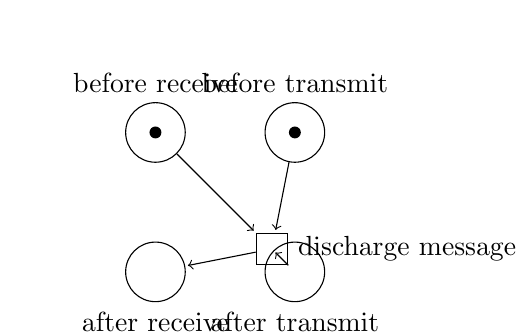
\begin{tikzpicture}
  \node[place,tokens=1,label=above:{before receive}] (beforeRx) {};
  \node[place,tokens=1,right = of beforeRx, label=above:{before transmit}] (beforeTx) {};
  \node[place,tokens=0,below=of beforeRx, label=below:{after receive}] (afterRx) {};
  \node[place,tokens=0,below=of beforeTx, label=below:{after transmit}] (afterTx) {};
  \node[transition,below right=of beforeRx, label=right:{discharge message}] (trans) {}
  edge [pre] (beforeRx)
  edge [pre] (beforeTx)
  edge [post] (afterRx)
  edge [post] (afterTx);
\end{tikzpicture}

Discharging a message here means copying the relevant bits of state from the transmitting thread's local state into the receiving thread's local state.
A message can be discharged if there is one thread willing to send it and one thread willing to receive it.
While the message is being discharged the two threads are effectively merged, with only one thread actually executing the message side effects.
Once the message is finished the two threads separate again and continue to execute independently.

A thread is only willing to receive a message if the message would pass the thread's message filter.
This has two parts:

\begin{itemize}
\item
  The message must have the correct message ID.
  This simply means that the send and receive parts of the message operation must be trying to enforce the same happens-before edge.
\item
  The message must pass the receiving thread's message receive filter.
  This filter consists of all of the side-conditions present in the crash enforcement plan which will become evaluatable once the message has been received.
\end{itemize}

However, in a real implementation, the threads are not pre-specified, and most of the complexity of the message algorithm lies in determining them.
When the plan demands that a message be sent or received, one side can be determined trivially, but the other must be discovered.
For a receive operation, the algorithm to do so in the abstract semantics looks like so:

\begin{algorithmic}[1]
  \If {$l$ has a bound thread}
    \If {The bound thread does not have an outgoing message}
      \State {Wait for it to send one}
    \EndIf
    \If {The bound thread has an outgoing message and it passes the message filter}
      \State {Discharge the message}
    \Else
      \State {$l$ has failed; remove it from the active set}
    \EndIf
  \Else
    \State {Examine the set of outstanding unbound message sends and collect all of the ones which pass the message filter into $s$}
    \State {Extend $s$ with $\bot$}
    \State {Choose $s'$ non-deterministically from $s$}
    \If {$s\prime = \bot$}
      \State {Register $l$ as a receiver of unbound messages}
      \State {Wait for the delay specified in this receive operation}
      \State {Unregister $l$ as a receiver of unbound messages}
      \State {Collect all of the unbound sends which pass the filter which started while we were waiting into $s$}
      \State {Select $s'$ non-deterministically from $s$}
    \EndIf
    \State {Discharge $s'$}
  \EndIf
\end{algorithmic}

The send operation is symmetric:

\begin{algorithmic}[1]
  \If {$l$ has a bound thread}
    \If {The bound thread is attempting to receive a message}
      \State {Wait for it to start receiving}
    \EndIf
    \If {The bound thread is receiving a message and this message would pass its filter}
      \State {Discharge the message}
    \Else
      \State {$l$ has failed; remove it from the active set}
    \EndIf
  \Else
    \State {Examine the set of outstanding unbound message receives and collect all of the ones whose filters this message would pass into $s$}
    \State {Extend $s$ with $\bot$}
    \State {Choose $s'$ non-deterministically from $s$}
    \If {$s' = \bot$}
      \State {Register $l$ as a sender of unbound messages}
      \State {Wait for the delay specified in this receive operation}
      \State {Unregister $l$ as a sender of unbound messages}
      \State {Collect all of the unbound receives whose filters this message would pass which started while we were waiting into $s$}
      \State {Select $s'$ non-deterministically from $s$}
    \EndIf
    \State {Discharge $s'$}
  \EndIf
\end{algorithmic}

As shown in figure ..., each message operation effectively defines an interval in time, and a send and receive match up if these windows overlap.
The behaviour when $s' = \bot$ is perhaps somewhat surprising: the thread waits a little while and then selects a peer thread to discharge the message with non-deterministically.
Meanwhile, all of the other threads are simultaneously performing similar non-deterministic choices.
The use of look-ahead nondeterminism means that all of the threads will make these selections in a mutually compatible way, so that there is no danger of A attempting to discharge its message with B while B discharges with C.
The actual implementation must resolve these constraints much more carefully, and is discussed in detail later.

Note that the message receive filter is evaluated as the message is being discharged, while the two threads are merged.
It is possible to imagine an alternative implementation in which the filter is instead evaluated locally in the receiver after the discharge operation is complete.
This would reduce the size of the synchronised section and so would appear, on the face of it, to offer greater parallelism, and hence potentially better performance.
Unfortunately, it does not work.
To illustrate the problem, consider again the example shown in figure \todo{...}.
One thread modifies a shared structure while another thread reads it, and the program will crash if the two threads happen to be operating on the same structure at the same time.
Suppose that the read thread runs far more often than the write one and that there are many instances of the structure.
The timeout balancing logic will quickly reduce the delay on the read side's first message send to zero and increase the delay on the write side's first message receive to compensate.
Now, when the write thread does run, it will stop just before \verb|l9| waiting for a matching read thread to arrive.
By hypothesis, many such threads will arrive, as the read thread runs more often than the write one.
In the alternative design, the read thread cannot evaluate the write thread's receive filter, and so every read thread will attempt to bind to the write thread, forcing the write thread to be duplicated many times.
Because of timeout rebalancing, the read thread will proceed from \verb|l2| immediately and quickly reach \verb|l5|, where it has to receive a message from \verb|l9|.
At this point, there are two possible outcomes:

\begin{itemize}
\item
  The thread is delayed at \verb|l5| waiting for the message from \verb|l9|.
  The write thread is still waiting in case any other threads reach \verb|l2| and attempt to synchronise with it, and so this might potentially be a rather long delay.
  Since the read thread runs far more often than the write thread, this will have a very large performance impact.
  Worse, it will probably be pointless: there, by hypothesis, a large number of instances of the structure which is being examined, and so, with high probability, the write thread will be modifying a different one.
  When the write thread does finally escape from its receive delay and evaluate its receive filter it will discover that the filter fails, and so the write thread will exit.
  The read thread will then discover that its bound thread has exited and be forced to exit as well.
  The crash enforcement plan will therefore not complete and the bug is highly unlikely to reproduce.
  
  Even worse, the performance hit might mean that the read thread will run far less frequently, further reducing the likelihood of the bug reproducing.
  In extreme cases, the attempt at enforcing a crash might actually make the bug less likely to reproduce in unit time.
\item
  The thread is not delayed at \verb|l5|.
  It never receives the message from \verb|l9| and must therefore exit without completing the plan, so is unlikely to reproduce the bug.
  The write thread's high-level interpreter will then accumulate a collection of low-level threads which have bound to exited read threads and which will themselves immediately exit.
\end{itemize}

Neither outcome helps to reproduce the target bug.

By contrast, in the scheme used by SLI, the read thread is able to evaluate the write thread's message receive filter at \verb|l2|.
It will therefore only bind to write threads which modify the structure which it is reading.
That means that the thread can be delayed a relatively long time at \verb|l5| without fear of apocalyptic performance damage, and so the bug will reproduce relatively easily.

\subsubsection{Discuss the timeout balancing bit}

Selecting the size of the various timeouts is important for determining the likelihood of reproducing a bug and the overheads of enforcing the patch.
SLI does so primarily dynamically, in response to the program's observed behaviour.

\subsubsection{Implementing non-deterministic choice in the Succ phase}

It might be that an instruction has several possible successors in the control flow graph in the crash execution plan, and in that case the interpreter must choose one of these successors using look-ahead non-determinism.
This cannot be implemented in any physically-realisable system, as it is non-causal, and so SLI must emulate it.
SLI uses a power-set construction to do so.
Rather than operating a single interpreter context, the actual implementation maintains a set of low-level interpreter contexts, which roughly follow the abstract semantics given above, and interprets them all in lock-step parallelism.
When one of these low-level interpreters needs to perform a non-deterministic choice between $n$ possible values, the high-level interpreter creates $n$ successor low-level interpreter states, one corresponding to each possible outcome of the choice, and inserts all of them into its current-state set.
They are then interpreted in parallel until enough information is available to resolve the earlier choice, at which point all but one of the threads will exit and the interpreter can revert to single-threaded execution.
If a thread is bound when it performs a non-deterministic choice then its bound thread must also be duplicated, to ensure that the new thread has something to bind to.

One subtlety here is that the original program's underlying instruction can only be retired once, and so the high-level interpreter must ensure that all low-level interpreters arrive at that point in the execution cycle at the same time.
SLI actually enforces a slightly stronger constraint, which is that every low-level interpreter in a given high-level interpreter must be at the same phase in the instruction execution cycle.
The only phases for which this is difficult are the message send and receive phases, which are discussed in more detail in the next section.

\subsubsection{Concrete implementations of message send and receive}

The message receive operation looks like this:

\begin{algorithmic}[1]
  \State {$lls \gets $ the set of currently-active low-level interpreter states}
  \State {$newLls \gets $ an empty set of low-level interpreter states}
  \For {$l$ in currently-active low-level interpreter states}
    \If {$l$ does not receive any messages}
      \State {Move $l$ from $lls$ to $newLls$ without changing it}
    \ElsIf {$l$ has a bound thread}
      \If {$l$'s bound thread has exited}
        \State {$l$ exits as well; remove it from $lls$ without adding it to $newLls$}
      \ElsIf {$l$'s bound thread has an outgoing message}
        \If {The bound thread's outgoing message passes the message filter}
          \State {Copy stashed values from the sending low-level interpreter's state to the receiving one}
          \State {Move $l$ from $lls$ to $newLls$}
        \Else
          \State {$l$ exits; remove it from $lls$}
        \EndIf
      \Else
        \State {} \Comment {Wait for a the bound thread to send a message}
      \EndIf
    \Else
      \State {} \Comment{Unbound receive}
      \For {$s$ registered unbound senders}
        \If {$s$'s outgoing message passes the message filter}
          \State {$l' \gets $ duplicate $l$}
          \State {$s' \gets $ duplicate $s$}
          \State {Copy stashed values from $s'$'s state to $l'$'s}
          \State {Bind $l'$ and $s'$ together}
          \State {Insert $l'$ into $newLls$}
          \State {Insert $s'$ into $s$'s high-level interpreter's active low-level interpreter list}
        \EndIf
      \EndFor
      \State {Register $l$ as an unbound receiver}
    \EndIf
  \EndFor

  \If {$lls$ is empty}
    \Return
  \EndIf

  \State {$end \gets now() + bound\_delay$}
  \If {There is a minimum delay}
    \State {Release lock}
    \State {Sleep for the minimum delay}
    \State {Acquire lock}
  \EndIf

  \While {There are bound receives in $lls$ and $now() < end$}
    \State {Release lock}
    \State {Wait for some bound receive to complete, or for the current time to pass $end$}
    \State {Acquire lock}
    \For {$l$ performing bound receives in $lls$}
      \If {$l$'s bound thread has exited}
        \State {Remove $l$ from $lls$}
        \State {$l$ exits}
      \ElsIf {$l$'s receiving-bound-message flag is clear}
        \State {Remove $l$ from $lls$}
        \State {Add $l$ to $newLls$}
      \Else
        \State Continue waiting
      \EndIf
    \EndFor
  \EndWhile

  \For {$l$ in $lls$}
    \If {$l$ is registered as an unbound receiver}
      \State {Unregister $l$ as an unbound receiver}
    \EndIf
    \If {$l$ was attempting a bound receive and the bound thread hasn't sent any messages}
      \State {Exit $l$}
    \ElsIf {$l$ is unbound}
      \State {The thread must have been attempting an unbound receive which failed, so exit $l$}
    \Else
      \State {} \Comment {Receive succeeded}
      \State {Add $l$ to $newLls$}
    \EndIf
  \EndFor

  \State {Set high-level interpreters set of currently-active low-level interpreters to $newLls$}
\end{algorithmic}

The send algorithm is very similar:

\begin{algorithmic}[1]
  \State {$lls \gets $ the set of currently-active low-level interpreter states}
  \State {$newLls \gets $ an empty set of low-level interpreter states}
  \For {$s$ in currently-active low-level interpreter states}
    \If {$s$ does not send a message}
      \State {Move $l$ from $lls$ to $newLls$ without changing it}
    \ElsIf {$s$ has a bound thread}
      \If {$s$'s bound thread has exited}
        \State {$s$ exits as well; remove it from $lls$ without adding it to $newLls$}
      \ElsIf {$s$'s bound thread is waiting to receive a message}
        \If {$s$'s outgoing message passes the message filter}
          \State {Copy stashed values from the sending low-level interpreter's state to the receiving one}
          \State {Move $s$ from $lls$ to $newLls$}
          \State {Clear the bound thread's receiving-bound-message flag}
        \Else
          \State {$s$ exits; remove it from $lls$}
        \EndIf
      \Else
        \State {} \Comment {Wait for a the bound thread to be ready to receive a message}
      \EndIf
    \Else
      \State {} \Comment{Unbound send}
      \For {$l$ registered unbound receivers}
        \If {The outgoing message passes $l$'s message filter}
          \State {$l' \gets $ duplicate $l$}
          \State {$s' \gets $ duplicate $s$}
          \State {Copy stashed values from $s'$'s state to $l'$'s}
          \State {Bind $l'$ and $s'$ together}
          \State {Insert $s'$ into $newLls$}
          \State {Insert $l'$ into $l$'s high-level interpreter's active low-level interpreter list}
        \EndIf
      \EndFor
      \State {Register $s$ as an unbound sender}
    \EndIf
  \EndFor

  \If {$lls$ is empty}
    \Return
  \EndIf

  \State {$end \gets now() + bound\_delay$}
  \If {There is a minimum delay}
    \State {Release lock}
    \State {Sleep for the minimum delay}
    \State {Acquire lock}
  \EndIf

  \While {There are bound sends in $lls$ and $now() < end$}
    \State {Release lock}
    \State {Wait for some bound send to complete, or for the current time to pass $end$}
    \State {Acquire lock}
    \For {$s$ performing bound sends in $lls$}
      \If {$s$'s bound thread has exited}
        \State {Remove $s$ from $lls$}
        \State {$s$ exits}
      \ElsIf {$s$'s sending-bound-message flag is clear}
        \State {Remove $s$ from $lls$}
        \State {Add $s$ to $newLls$}
      \Else
        \State Continue waiting
      \EndIf
    \EndFor
  \EndWhile

  \For {$s$ in $lls$}
    \If {$s$ is registered as an unbound sender}
      \State {Unregister $s$ as an unbound sender}
    \EndIf
    \If {$s$ was attempting a bound send and the bound thread hasn't tried to receive any messages}
      \State {Exit $s$}
    \ElsIf {$s$ is unbound}
      \State {The thread must have been attempting an unbound send which failed, so exit $s$}
    \Else
      \State {} \Comment {Send succeeded}
      \State {Add $s$ to $newLls$}
    \EndIf
  \EndFor

  \State {Set high-level interpreters set of currently-active low-level interpreters to $newLls$}
\end{algorithmic}

One further optimisation, not shown here, avoids redundantly duplicating low-level interpreter contexts in the common case that a message operation is discharged precisely once.

\todo{This is probably not the best way of presenting those
  algorithms.}

\todo{Discuss setting minimum delays here}

\subsubsection{The await-bound-thread-exit state}

When a thread completes its plan, it is sometimes useful for it to wait for its bound thread to exit before proceeding.
This is because the crash summary from which the plan is generated does not have complete information on the structure of the program.
If the last edge in a happens-before graph is from memory access A to memory access B, that generally means that A is a store and B is a load and B must load the value stored by A.
That means that, not only must B happen after A, but B must happen before any other writes to the memory location modified by A.
If there were other stores to that location in the crash summary then the happens-before graph would include additional edges to ensure that that happens, but if there are stores outside of the summary then it will not.
For instance, suppose that the write thread looks like this:

\begin{verbatim}
while (1) {
l1:  *x = 5;
l2:  *x = 7;
     <something_complicated>
}
\end{verbatim}

And the read thread looks like this:

\begin{verbatim}
l3: a = *x;
l4: b = *x;
    crash if a != b;
\end{verbatim}

This program is clearly buggy.
One way of reproducing this bug would be to interleave instructions as \verb|l1|, \verb|l3|, \verb|l2|, \verb|l4|.
SLI will discover this interleaving as the happens-before graph show in figure \todo{...}.
The algorithm described so far will be sufficient to enforce this graph (assuming that the two fragments of code shown can actually execute in parallel).
This is not, however, sufficient to cause the program to crash, because the generated happens-before graph is incomplete: it misses the edge from \verb|l4| to \verb|l1| in the next iteration of the loop.
If the loop completes and reaches the store at \verb|l1| before the load \verb|l4| completes then the bug will not reproduce even though the happens-before graph was successfully enforced.
Any scheme with an analysis horizon based on a simple instruction count will suffer from a similar problem, but this is particularly serious for SLI, because the delays inserted are in almost precisely the right place to maximise the chance of this kind of bug-hiding race.
Returning to the example, SLI's crash enforcement plan will include a delay after \verb|l1| (to implement the \verb|l1| to \verb|l3| happens-before edge), and this delay will be large relative to a short sequence of normal instructions, and so the bug will be hidden completely provided that the delay to wake up the read thread after the final edge is greater than the time taken to execute \verb|<something_complicated>|.
This is perfectly plausible, given that \verb|<something_complicated>| only needs to be a few dozen instructions to exceed SLI's analysis window.
This bug will therefore never reproduce under SLI's crash enforcer, even when the happens-before graph is enforced perfectly.
The fix is simple: have the store thread delay slightly after completing its final message send operation, until the read thread also completes its crash enforcement plan.
This ensures that activity beyond the analysis horizon cannot prevent bug reproduction, and, because it only happens when the plan is mostly complete, and hence happens very rarely, it has very low performance overhead.

\begin{tikzpicture}
\node[CfgInstr] (l1) {l1};
\node[CfgInstr, below = of l1] (l2) {l2};
\node[CfgInstr, right = of l1] (l3) {l3};
\node[CfgInstr, below = of l3] (l4) {l4};
\draw[->] (l1) -- (l2);
\draw[->] (l3) -- (l4);
\draw[->,happensBeforeEdge] (l1) -- (l3);
\draw[->,happensBeforeEdge] (l3) -- (l2);
\draw[->,happensBeforeEdge] (l2) -- (l4);
\end{tikzpicture}


\subsubsection{Compiling the plan}

\todo{Implementation of this is currently massively broken; need to
  decide whether I'm going to fix it or just use a slightly older
  version.}

In addition to a plan interpreter, SLI also includes a plan compiler, which combines the plan with the program's original machine code to produce a modified version of the program which performs the necessary enforcement actions without needing an interpreter.
The intent here is to reduce the overhead of the interpreter in the case where SLI is investigating many bugs most of which do not exist.
Making this practical requires several simplifications to the semantics:

\begin{itemize}
\item
  The number of physical program threads operating in the plan is limited.
  In particular, it is assumed that only one program thread will be executing the read side of the plan at any time, and likewise only one thread will be executing the write side.
\item
  The message semantics are simplified: messages are sent asynchronously, with a delay only on the read side, and must be ``cancelled'' when the relevant thread exits.
  This has two important implications: first, that a message send can never fail and, second, the something must keep track of what messages a given thread currently has outstanding.
  Combined with the first simplification, it also means that at most one instance of any given message can be outstanding at any one time, and so it is easy to place the relevant information in a global structure without needing any dynamic memory allocation.
\item
  High-level interpreter contexts only ever access the state of their own low-level interpreters.
  This has two important implications:

  \begin{itemize}
  \item
    Remote low-level interpreters are never duplicated during message operations.
    If the normal semantics would require an interpreter to be duplicated then the local message operation fails.
  \item
    The receive message filter can only be executed by the receiving thread after receiving a message.
  \end{itemize}
\item
  When a low-level interpreter is duplicated due to a non-deterministic choice in the Succ phase the low-level state's stash table is not duplicated.
  Instead, all low-level interpreters in a given high-level interpreter share a single stash table.
\end{itemize}

The result is a system with lower run-time overheads, but also a lower probability of reproducing interesting bugs.
It has a much larger I-cache footprint but a smaller D-cache one\editorial{Not sure where I'm going with that, although it is true and kind of interesting}.

I now briefly outline the implementation of this compiler.
The core idea is to compile the CFG in the enforcement plan into a state machine.
This state machine consists of a large number of smaller intra-instruction state machines, as illustrated in figure~\todo{...}, each of which models a single instruction in the original program.
The label on each state is itself a set of low-level labels which consist of a four-tuple of the plan thread which is executing, a reference to the plan CFG node, a set of messages which have been sent by the thread, and the phase of the intra-instruction state machine.
Each state is compiled to a small fragment of machine code (which might be empty, if this instruction does not have an relevant annotation in the plan) plus a set of relocations specifying the fragment's relationships to the other states.
Once every state has been compiled these relocations can be discharged and the fragments concatenated together to form the final patch.

I now discuss the details of each phase of the intra-instruction machine:

\begin{itemize}
\item[RecvMsg]
  Examine the set of CFG nodes which are active in the current state and determine whether the plan requires any of them to receive messages.
  If so, emit code to examine the global outstanding-message structures to see whether of the desired messages are currently outstanding.
  If there are, receive precisely that message.
  Any other message receive operations are considered to have failed and the relevant CFG nodes removed from the current state label.
  If no message sends are currently outstanding then the physical thread is delayed until either one is available or some timeout is reached.
  If a message becomes available then it is received, and otherwise all receives fail and all receiving CFG nodes are removed from the label.
  Note that this does not necessarily mean that the state label will become empty\footnote{Although that is the common case.} as there may be some CFG nodes which do not need to receive messages.

  Once a message is received its content is simply copied from the global message area into the local thread's stash area.
\item[OrigInstr]
  Store any generated values into simulation slots and issue the original instruction.
  There are three main cases to consider here:

  \begin{itemize}
  \item
    Simple memory loads.
    If the instruction is of the form \verb|LOAD *location -> register|, and the value loaded is to be saved, then it is sufficient to just copy \verb|register| into the simulation slot after the original instruction has completed.
  \item
    Compound memory loads.
    Instructions which load from memory but are not themselves simple loads are more difficult to handle.
    For concreteness, suppose that the instruction is \verb|CMP 76,*loc1|, and the annotation requires us to save the value loaded.
    The instruction loads from \verb|*loc1| but does not leave the result in any locations which we can easily access.
    It would be possible to solve this problem by adding another load of \verb|*loc1|, but that would run the risk of a store in a remote thread modifying \verb|*loc1| between the two loads, leading to very confusing results.
    SLI instead solves this problem by rewriting the instruction to this:

\begin{verbatim}
LOAD *loc1 -> reg1
STORE reg1 -> simslot
CMP 76, reg1
\end{verbatim}

    This exposes the loaded value to the instrumentation framework, allowing it to be stored to the simulation slot as desired.

    Instructions which modify memory in-place, such as \verb|ADD 1 + *loc1 -> *loc1|, pose a similar problem and can be solved in the same way, provided that they do not have a \verb|LOCK| prefix.
    \verb|LOCK|ed instructions are more complex, as separating the load and store phases into separate instructions would violate the semantics of the program and might introduce new bugs.
    SLI solves this problem using a \verb|CMPXCHG| loop.
    For instance, the instruction \verb|LOCK ADD 1 + *loc1 -> *loc1| would be converted to this machine code fragment:

\begin{verbatim}
1: LOAD *loc1 -> reg1
ADD 1 + reg1 -> reg2
LOCK CMPXCHG *loc1, reg1 -> reg2
if_cmpxchg_failed goto l1
STORE reg1 -> simslot
\end{verbatim}

    The \verb|CMPXCHG| instruction here is supposed to be an invented syntax for the x86 machine code instruction which atomically compares \verb|*loc1| to \verb|reg1| and, if they are equal, sets \verb|*loc1| to \verb|reg2|.
    This allows SLI to expose the value of the implicit load while preserving the \verb|LOCK| semantics of the original instruction.
  \item
    Branch instructions are deferred to the FindSucc state.
  \end{itemize}
  
\item[SendMsg]
  Send any outgoing messages.
  This amounts to simply copying the message payload into the global message area, setting a global flag to indicate that the message is currently outstanding, and adding the message ID to the state label's set of sent messages.
  This always succeeds and advances to the FindSucc state.

\item[ExitThread]
  When a low-level thread exits it is necessary to cancel any messages which it has sent.
  The compiler takes the union of all of the sent-messages sets in its low-level, removes the thread which is to exit, and then takes the union again.
  Any messages present in the first set but not the second need to be cancelled by setting the relevant global message-outstanding flag to zero.
  The compiler will then either exit the patch, if the last low-level thread has exited, or resume the intra-instruction state machine at an appropriate place.
\end{itemize}


\begin{tikzpicture}
\node[flowChartState] (RecvMsg) {RecvMsg};
\node[flowChartState,above left = of RecvMsg] (StartThread) {StartThread};
\node[flowChartState,above right = of RecvMsg] (CheckForThreadStart) {CheckForThreadStart};
\node[flowChartState, below = of RecvMsg] (OrigInstr) {OrigInstr};
\node[flowChartState, below = of OrigInstr] (VerfCond) {VerfCond};
\node[flowChartState, below = of VerfCond] (SendMsg) {SendMsg};
\node[flowChartState, below = of SendMsg] (FindSucc) {FindSucc};
\node[flowChartState, right = of VerfCond] (CondFail) {CondFail};
\node[flowChartState, right = of CondFail] (Exit) {Exit};
\node[flowChartState, left = of RecvMsg] (RecvdMsg) {RecvdMsg};
\draw[->] (CheckForThreadStart) -- (RecvMsg) -- (OrigInstr) -- (VerfCond) -- (SendMsg) -- (FindSucc);
\draw[->] (StartThread) to [bend right=10] (CheckForThreadStart);
\draw[->] (CheckForThreadStart) to [bend right=10] (StartThread);
\draw[->,dashed] (FindSucc.east) to [bend right=75] (CheckForThreadStart.east);
\draw[->] (RecvMsg) -- (RecvdMsg) -- (OrigInstr);
\draw[->] (RecvMsg) -- (Exit);
\draw[->] (VerfCond) -- (CondFail) -- (Exit);
\draw[->] (FindSucc) -- (Exit);
\end{tikzpicture}

  

\subsubsection{Compiling entry point stubs}
\label{sect:find_bugs:compile_entry_points}

\todo{Good Lord, this is completely incomprehensible.}

The entry points of the crash enforcement plan are given as mappings from call stacks to CFG nodes.
The program must be patched so that it transfers control to the interpreter whenever the call stack matches up with one of these entry-point call stacks.
This is a multi-step process:

\begin{itemize}
\item
  The last pointer in the call stack is a raw instruction pointer.
  The relevant instruction is patched into a jump into the interpreter trampoline.
\item
  The interpreter trampoline transitions to a different stack, saves the client program's register state, and starts the main interpreter.
\item
  The main interpreter then examines the program's stack to determine whether it matches up with the entry-point stack.
  If it does then a new high-level interpreter state is created and interpretation starts.
  Otherwise, the interpreter exits back to the original program (possibly after emulating enough instructions to avoid returning into the middle of the new jump instruction).
\end{itemize}

The last point is more subtle than it might appear, as the interpreter must be able to find arbitrary return addresses on the program's stack, and this is difficult if the program is compiled without frame pointers or debug symbols.
SLI uses a static analysis, performed when generating the crash enforcement plan, to solve this problem.
The static analyses already described are sufficient to determine the entry point of the function containing a given RIP, and so it is easy to perform a simple abstract interpretation forwards from that point to the given RIP and hence find the number of bytes which the function will push onto the stack on the way\footnote{This is generally fixed for all possible paths}.
The first entry in the call stack is trivially true because of the way the jumps are patched in.
The second one is the return address of the current function, which can be found using that offset.
The third one is the return address of the calling function, and the offset there is just the previous offset plus the offset in the calling function.
In this way all necessary offsets can be found and the entry-point stack checked completely.

\subsubsection{Run-time considerations}

Recovery from spurious segfaults in the patch due to e.g. LD operations.

\subsection{Comparison to schedule memoisation}
\subsection{Comparison to STM block inference stuff}

\section{Fixing bugs}

\subsection{Using global locks}
\label{sect:fix_global_lock}

In addition to finding bugs, SLI can also be used to fix them in a
largely automated fashion.  The basic approach here is to binary patch
the program to introduce a new global lock covering the program's
relevant instructions, preventing them from executing in parallel and
hence preventing the bug from occurring (assuming that the relevant
instructions have been correctly identified).  The relevant
instructions are duplicated into a binary patch, unrolling loops and
tracing across function boundaries in a way which reflects the
function inlining and loop unrolling performed during the initial CFG
generation phase, and the duplicates modified to acquire and release
the lock at appropriate points.  The original program is then patched
branch to the duplicates when necessary.

The first step in producing such a fix is correctly identifying the
instructions which must be included in the critical sections.  These
will be roughly a subset of the instructions involved in the
control-flow graphs associated with \StateMachines; a subset because
some instructions in the CFG do not need to be protected, and roughly
because some instructions not in the CFG will also be included in the
critical section.

As an example of the former, consider a program like this:

\begin{verbatim}
read_side() {
    ptr = complicated_local_calculation();
    dptr = *ptr;
    if (dptr != NULL) {
       dptr = *ptr;
       *dptr = 5;
    }
}
write_side() {
    ptr = complicated_local_calculation();
    *ptr = NULL;
}
\end{verbatim}

Here, the read thread computes some pointer using entirely local
operations, loads from it once and then, if the result is
non-\verb|NULL|, loads from it again and uses the resulting pointer.
Meanwhile, the store thread sets a potentially coincident memory
location to \verb|NULL|.  The read thread clearly has a potential
time-of-check, time-of-use race bug.  The \StateMachines generated by
SLI will include the buggy code itself but might also include part or
all of \verb|complicated_local_calculation()| and a side-condition
which requires the two pointers to match up.  This extra information
is useful when analysing the bug (\needCite) or when attempting to
reproduce it (\needCite) but cannot be used by this kind of
instruction-level fix\footnote{But see future work section~\needCite
  for a possible alternative scheme which would make use of it.}, so
including it in the fix is unhelpful and would tend to lead to
unnecessarily large critical sections.  The fix generating process
must therefore select a useful subset of the instructions in the
control-flow graph.

The approach taken here is simple:

\begin{itemize}
\item
  Reduce the verification condition from the bug summary until it
  contains only happens-before edges.  These entirely capture the
  instruction-interleaving parts of the bug to be fixed, and, since
  instruction-interleaving is the only thing which can be influenced
  by this type of patch, the resulting condition contains all of the
  useful information in the condition.
\item
  Identify all of the CFG nodes which are mentioned in one of those
  happens-before edges.
\item
  Trim the CFG such that every path starts and ends in one of those
  mentioned nodes.  All such paths will be included in a critical
  section, and so no such paths will be permitted to execute in
  parallel.
\end{itemize}

In this way the CFG is restricted to just those instructions which are
involved in the interleaving which is to be prevented.

Note that this is not guaranteed to produce an optimal selection of
critical sections, in the sense that sections can sometimes be larger
than is strictly necessary.  Consider, for example, a program with the
same read side as the previous example but a write side in which the
pointer is assigned to twice:

\begin{verbatim}
write_side() {
    ptr = complicated_local_calculation();
    *ptr = NULL;
    *ptr = NULL;
}
\end{verbatim}
    
There are now two obvious ways of protecting this program:

\begin{itemize}
\item
  Place both loads in the read side in a single critical section and
  both stores in the write side in another one.
\item
  Place both loads in the read side in a single critical section, but
  give each store in the write side its own critical section.  In
  other words, drop and re-acquire the lock in between the two stores.
\end{itemize}

Both approaches correctly eliminate the bug, but they will have
different performance characteristics.  In particular, dropping and
re-acquiring the lock reduces the size of the critical section, which
might improve concurrency and reduce starvation, but imposes higher
overheads due to the greater number of lock operations.  In principle
the happens-before graph implicit in the verification condition
contains enough information to determine whether dropping the lock is
safe, but, in this mode, SLI does not make use of this information,
and always uses the former strategy\footnote{But
  see~\ref{sect:fix_from_drs} for a mode in which it can use the other
  approach.}.

Once the relevant fragment of CFG has been identified, entry point
stubs must be generated and the program patched to branch to them at
appropriate points.  There are two main complications here:

\begin{itemize}
\item
  Instructions on x86 are not all the same size, and, in particular, a
  branch instruction is larger than some of the instructions which
  need to be patched.  This means that replacing an instruction with a
  branch to a patch entry point stub might clobber the following
  instruction; if there are any branches to that instruction from
  anywhere else in the program then the results are unlikely to be
  helpful.
\item
  The control-flow graphs used by SLI can cross function boundaries,
  and in particular are sometimes only valid in a particular function
  call context.  The patch must therefore check that the stack matches
  before attempting to run the CFGs.  Note, in particular, that
  whereas stack context checking is a performance optimisation when
  trying to trigger bugs it is necessary for correctness when trying
  to prevent them.
\end{itemize}

SLI solves the first problem by expanding the critical sections
backwards so that they do not start on dangerous instructions.  The
early static analysis passes discover all of the branches within the
program, and so can detect when inserting a branch would cause a
dangerous clobber, and in that case it simply expands the critical
section to include the instruction's predecessors\footnote{This might,
  of course, mean that the critical section has multiple entry points;
  that is not a problem.}.  The process then iterates until a safe
instruction is found\editorial{What if no safe instruction is found
  e.g. a loop with no suitable instructions in?  That does actually
  work, but, thinking about it, I'm not entirely certain why; should
  check that.}.  One complication here is branches from libraries into
the main program, which will not be detected by the static analysis.
Fortunately, they are detected by the dynamic analysis, and so this is
not a problem\editorial{Assuming that the dynamic analysis is
  complete, which is kind of a big assumption.  Saying that we miss
  some bugs when the analysis is incomplete is one thing; saying that
  we introduce more is a bit more of a big deal.  Probably need to say
  a bit more about that.}.

This problem was also tackled by the AutoPaG project, and the solution
they developed is similar. \todo{Similar but not the same.  They use a
  dominator-based scheme, and hence avoid needing the global branch
  information but can end up with much larger patches and a higher
  risk of deadlocks/starvation problems.  The original version of SLI
  used basically the same algorithm (although I did it first); should
  probably explain why I had to switch.}

The second problem, checking function call contexts, is much simpler,
and SLI solves it by simply emitting machine code to perform the
appropriate checks (using a stack layout derived in the same way as in
\S~\ref{sect:find_bugs:compile_entry_points}) and branch to an
appropriate place in the patch (or return to the original program if
there is none).  One subtlety here is that the original instruction
will have been replaced by a branch, and so returning to it directly
is unlikely to be effective, and so SLI copies the branch into the
patch (and possibly also a small number of clobbered instructions, if
necessary) and executes them from the patch before returning, without
holding the patch lock.\editorial{Rewrite the whole damn paragraph.}

An alternative approach would be to take control of the program using
debug breakpoints rather than jump instructions.  These are either a
single byte (for the \verb|int3| instruction) or no bytes at all (for
debug registers), and so avoid the instruction clobbering problem.
This would work, but would have a couple of important disadvantages:

\begin{itemize}
\item
  Debug breakpoints are far slower than branches.  This might be
  important if the critical section is to be inserted on a
  particularly hot code path.
\item
  Using debug breakpoints in this way would interfere with any other
  debugger which the developer might want to use.  With a branch-style
  patch, standard debuggers work without modification for any part of
  the program which has not been patched, whereas a breakpoint-style
  patch requires extensive coordination between the debugger and the
  patch mechanism for either to work at all.
\item
  Breakpoint registers are of strictly limited number on most
  architectures (four, on x86).  This means that they can never
  provide a complete solution by themselves.
\item
  On most UNIX-type operating systems, including Linux and FreeBSD,
  catching debug breakpoints requires modifying the program's signal
  handling configuration, which requires some level of coordination
  with the program to be modified.  It would be possible to use an
  alternative API, but this would require kernel modifications,
  complicating the use of the generated patches\footnote{Branch-style
    patches also require modifying signal handling configurations in
    order to, for instance, provide a correct faulting instruction
    address in SIGSEGV register configurations.  However, very few
    programs actually require that information for correctness, and so
    it is not usually a major issue if the patch loses control of the
    signal handler to the main program.  In a breakpoint-style patch,
    losing control of the signal handler means, first, that the patch
    is never run, and so cannot hope to fix the bug, and, second, that
    the program receives spurious breakpoint events, which will often
    introduce additional erroneous behaviour.}.
\end{itemize}

SLI therefore generates predominantly branch-style patches.

\todo{I did implement a breakpoint-based scheme, so it might be
  interesting to actually include some numbers on their relative
  effectiveness.}

\subsection{Other ways of fixing the bugs}
\todo{I've come up with an algorithm for doing this using a message
  passing network, like we do for crash enforcement but with the
  delays in slightly different places, but I really don't have time to
  implement it.  It is kind of cool, though; I'd like to include it
  somewhere, even if it's just a future work-type thing.}

\todo{Might also be worth saying a few words about possibly fixing the
  bugs by using STM-like techniques?  I've not implemented any of
  them, either, but they are kind of interesting.  Probably worth a
  paragraph or two.}

\section{Fixing bugs from DRS logs}
\label{sect:fix_from_drs}
The simplest way to fix a bug is to start from a DRS log.
Given a log, identifying the thread and which is most responsible for a crash is generally straightforward.
If the crash is caused by dereferencing a bad pointer then the responsible thread is the one which dereferenced the pointer; if the crash is an assertion failure then the responsible thread is the one which called \verb|abort()| (or equivalent).
The log then makes it trivial to determine what instructions the responsible thread executed before it crashed, and a suffix of these can be compiled into a \StateMachine capturing the most relevant parts of the responsible thread's behaviour.

The log also makes it trivial to determine precisely which stores the read-side thread raced with, and so building a write-side \StateMachine is redundant.
Instead, the read-side \StateMachine is ``slid across'' the log, evaluating it at every step (subject to some typing constraints which ensure that the result is reasonable), and the resulting pattern of safe and unsafe regions converted directly into critical sections, without ever needing to generate an explicit write-side \StateMachines.

\subsection{Building the read-side \StateMachine}
\todo{This is gratuitously different from the non-DRS mode in an enormous number of places.  I should fix that.}

Working from a DRS log provides a lot of information which is not available in SLI's normal mode of operation.
This makes some parts of the algorithm redundant.
In particular, there is no need to generate large numbers of CFGs of fragments of the program which might be relevant, as we know precisely which instructions were executed leading up to the crash.
Instead, in this mode, SLI generates the \StateMachine directly from the log.
It starts with a small stub machine representing just the instruction which crashed and then expands it backwards, incorporating a single instruction from the log at a time.
For instance, suppose that the fragment of program to be investigated looked like this:

\begin{verbatim}
l1: mov $5, %rax
l2: mov (global1), %rbx
l3: mov (%rax + %rbx), %rcx
\end{verbatim}

and the program crashed due to dereferencing a bad pointer at \verb|l3|.
The initial stub \StateMachine will then be just:

\begin{verbatim}
if (BadPtr(rax + rbx)) crash(); else survive();
\end{verbatim}

Incorporating \verb|l2| will transform that to

\begin{verbatim}
LOAD (global1) -> rbx
if (BadPtr(rax + rbx)) crash(); else survive();
\end{verbatim}

Incorporating \verb|l1| will then produce the \StateMachine

\begin{verbatim}
COPY 5 -> rax
LOAD (global1) -> rbx
if (BadPtr(rax + rbx)) crash(); else survive();
\end{verbatim}

Which can be simplified in the usual way to produce

\begin{verbatim}
LOAD (global1) -> rbx
if (BadPtr(rbx)) crash(); else survive();
\end{verbatim}

And this can then be used in the rest of the analysis.

The major subtlety here lies in the handling of control flow, and the parts of the program which are not executed.
One possible approach would be to simply say that any changes to the control flow cause the bug to be avoided, but this is over-optimistic.
Consider, for instance, a program like this one:

\begin{verbatim}
ptr = global;
if (some_condition)
    idx = 1;
else
    idx = 2;
local = ptr[idx];
\end{verbatim}

This program loads a pointer to an array from a global variable and then loads some index in the array, with the index chosen depending on some condition.
Suppose that the race then causes the pointer in \verb|global1| to sometimes be bad, and that the reproduction of the bug was obtained while \verb|some_condition| holds.
The bug itself does not depend on \verb|some_condition|, but if one were to assume that any changes to control flow avoid the bug then SLI would not be able to show this.
This problem can only be avoided by exploring untaken branches, and SLI does so, for some (configurable) number of instructions.
If the control flow rejoins that which is represented in the DRS log then an appropriate branch is included from one part of the \StateMachine to another, and if it does not rejoin then a branch to the \verb|NoCrash| state is used instead.

One complication here is that a given static instruction might be represented multiple times in the DRS instruction trace, and hence multiple times in the \StateMachine, if the instruction is part of some loop.
This makes it ambiguous where the branch should branch to.
SLI solves this problem by taking the earliest instance of the instruction, and hence branching to the place in the \StateMachine nearest the root.
This helps to keep the loop structure of the program intact, subject to the unrolling implicit in the DRS log.

The example shown above might then turn into a \StateMachine something like this:

\begin{verbatim}
LOAD global1 -> ptr
if (some_condition) {
   COPY 1 -> idx1
} else {
   COPY 2 -> idx2
}
if (BadPtr(ptr + idx)) {
   crash();
} else {
   survive();
}
\end{verbatim}

The standard simplified will then transform that to this:

\begin{verbatim}
LOAD global1 -> ptr
if (BadPtr(ptr + (some_condition ? 1 : 2))) {
   crash();
} else {
   survive();
}
\end{verbatim}

SLI uses a rule that \verb|BadPtr(x + k)| is equivalent to \verb|BadPtr(x)| whenever \verb|k| is a small constant, and so correctly determines that the bug is independent of \verb|some_condition| in this case.

\todo{Discuss using more powerful bug definitions here e.g. Valgrind, invariant discovery, etc, by applying them to the log and then converting to stub machines, so that you can apply this to races which lead to bugs other than immediate bad pointer dereferences.}

\subsection{Requirements on the DRS}

\subsection{Finding remote critical regions}

The fixes generated by SLI rely on making the read-side \StateMachine operate as-if atomically and then ensuring that it does not execute in any states where doing so would lead to a crash.
In the normal mode of operation, the regions which would lead to a crash are determined by modelling the rest of the program as a set if write-side \StateMachines and then using symbolic execution, but it is possible to be more accurate\editorial{or possibly precise?} if a full DRS log is available.
Instead of the set of \StateMachines, the log itself can be used as a model for the rest of the program.
The idea here is that the log contains a sequence of possible states of the program, and contains all of the ones which are relevant to this particular way of reproducing the bug of interest.
SLI therefore slides the read-side \StateMachine over this log, evaluating it at every instruction, and hence classifies the log into ``safe'' and ``unsafe'' regions, and the transitions between these two types of region give the boundaries of the write-side critical regions.

As a minor optimisation, SLI only re-evaluates the \StateMachine if there has been a store to some memory location which is loaded by the \StateMachine.
This cannot affect the results in any way, but means that the \StateMachine does not have to be evaluated as often.

One important complication here is the presence of dynamically-allocated data structures.
SLI relies on being able to identify points in the program where these are allocated and released.
The loads in the read \StateMachine will correspond to specific load operations in the DRS log and SLI is then able to check which dynamic instance of structures those accesses access and will only evaluate the \StateMachine while all of the relevant structures remain live.

Once the log has been classified, the classification must be converted into realisable critical sections.
In other words, SLI must identify points in the program at which it must insert lock acquire operations and points where it must insert lock release operations.
Ideally, each unsafe region in the log would correspond to a single critical section, with a single acquire operation and a single release one.
This can fail in several ways:

\begin{itemize}
\item
  The start and end of the unsafe region might be in different threads, if, for instance, one thread violates an invariant and another thread then restores it.
  It is difficult to model a cross-thread operation as a critical section.
  SLI cannot prevent this kind of bug, and the unsafe region is simply ignored.
\item
  There might be non-trivial control flow between the start and end of an unsafe region within a single thread.
  In that case additional acquire and release operations must be inserted to ensure that locks are not leaked, double-acquired, or double-released.
\item
  The program might have additional synchronisation mechanisms which, when combined with the SLI-inferred synchronisation, lead to a deadlock.
\end{itemize}

These are discussed in more detail in \S~\ref{sect:fix_global_lock}.

\todo{This is in dire need of rewriting.}

Note that the definition of a dynamic structure is somewhat subtle here.
Most obviously, \verb|malloc| and \verb|free| represent boundaries in the lifespan of such structures (with \verb|malloc| being the start and \verb|free| being the end), but ``re-typing'' operations can also impose such boundaries.
The intent of the sliding procedure is to capture other operations which the program might perform on the data structures involved in the synchronisation bug, in the same way that write-side \StateMachines do in the non-DRS case.
In effect, the program's behaviour is constrained using a heuristic memory safety property, and this memory safety property must correspond reasonably closely to the program's actual structure.

The underlying hypothesis here is that the program has some kind of internal type system which constrains which operations will be performed on a given memory location.
This means that two pieces of code can only race if they have types which are in some sense compatible, so that they might access overlapping memory locations.
The combination of the read-side \StateMachine and the set of dynamic instances accessed by it defines, in a slightly ill-defined way, a set of types which the read side of the critical section might access.
SLI must then find some other operations on the same types to synchronise against, and this is the aim of the sliding procedure.
In order for this to work, the read \StateMachine must only be slid to places where the current types match up with the types for which it was derived.
SLI must therefore be able to identify points where the types of memory locations change.
This includes things like \verb|malloc| and \verb|free|, but is also likely to include things like program-specific memory allocators or object pools.
The precise set will depend on the program's type system, and so can only be sensibly modelled with assistance from the programmer.




\chapter{Evaluation}
\section{Things to evaluate}

What I have:

\begin{itemize}
\item About a dozen artificial bugs for each mode
\item The glibc bug kernel --- fixed in DRS mode
\item The Thunderbird bug -- fixed in DRS mode
\item The first mysql bug -- fixed in core dump mode
\item The second mysql bug -- found and fixed in whole-pass mode
\end{itemize}

And that's about it.
Where I've said a bug is fixed or found in one mode that indicates that I've tested and confirmed that it works in that mode; it doesn't say anything about whether it would work in one of the other modes.

So I desperately need more real bugs.
Possible ways of getting them:

\begin{itemize}
\item
  enforce\_crash.
  I need to go and apply this to as many programs as possible, which will hopefully give me something more to work with.
\item
  Take an existing program and rip out the synchronisation, then see if we can find the resulting bugs.
  STAMP would be a reasonable place to look here.
\item
  Another bug tracker crawl.
  This would be bloody tedious but might turn up something.
\end{itemize}

Other things I can look at and evaluate:

\begin{itemize}
\item
  Turn the various simplification passes on and off and see what effect that has.
\item
  CDF of how long analysing a given potentially-crashing instruction takes.
\item
  Look at different strategies for combining machines.
\item
  Look at effect of different analysis window sizes: how many bugs do we find, how many false positives, how much time does the analysis take.
\item
  Compare the CFG-based approach to building machines to the old backtracking one.
\item
  Direct eval of the effectiveness of the induction rule.
\item
  Look at how many bugs are killed off by the different clauses of the crash definition.
\item
  Cross-eval of the accuracy of the static analysis passes by doing a dynamic analysis which checks their predictions.
\item
  Investigate performance hit of the enforcement mode, and how that depends on the mechanism used to generate the enforcers.
\item
  Compare compiled enforcers to interpreted ones.
  Performance, number of bugs detected, cost of building the damn things.
  Relative I- and D-cache footprints.
\item
  How much does the W isolation property actually buy us, in terms of analysis cost?
  How much does it cost us, in terms of lost bugs?
\item
  How large are the CFGs and \StateMachines which we actually generate?
  Also, how large are the intermediate machines generated when we're generating verification conditions?
\item
  Do we actually win anything from using the slightly odd form of SSA?
\item
  We handle multi-rooted CFGs completely differently between read and write modes.
  Does that win/lose anything?
\item
  There's almost certainly something to say about the dynamic analysis phase, probably to do with how quickly it converges.
\item
  Might also be able to say something about how complex the resulting aliasing tables are.
\item
  Look at how long the various phases take.
\item
  There are a bunch of places where we have to decide between using the simplifier and the sat checker.
  Eval which works better for each of them.
\item
  When you're doing the cross-product machines you have a choice between explicit and implicit happens-before edges.
  Explicit is basically always better; figure out how much by, and why.
\item
  Crash enforcement: timeout strategies.
\item
  Crash enforcement: how useful is side-condition checking?
\item
  Crash enforcement: how often do we redundantly evaluate side conditions?
\item
  Crash enforcement: Is await-bound-exit actually useful?
  We know it is in silly little artificial test cases, but perhaps not in real programs?
\item
  Artificially limit number of live assertions to 5.
  Investigate what effect that has.
\end{itemize}

\subsection{Validation of tool implementation}

\subsubsection{Cross-thread stack accesses}

\subsubsection{Static analyses}

SLI relies on two forms of whole-program static analysis applied to the target binary before the main analysis starts:

\begin{itemize}
\item
  The simple points-to analysis.
\item
  An analysis to recover the offset between RSP and RBP, where that is a constant.
\end{itemize}

Both analyses assume in at least some places that the program to be analyses conforms to the system ABI.
If that assumption does not hold, or if there is simply a bug in one of them, then that might invalidate all of the other results.
I therefore developed some Valgrind-based dynamic analyses to check that the results of this phase were correct.

\subsubsubsection{Points-to analysis}

The static points-to analysis builds an instruction attribute table for the program which includes, for each instruction:

\begin{itemize}
\item
  Whether the current stack frame might include any pointers to itself.
\item
  Whether there might be any pointers to the current stack frame in memory which is not part of the current stack frame.
\item
  For each register, a flag saying whether that register might point at the current stack frame.
\end{itemize}

The ``current stack frame'' here is defined to be the region of memory between \verb|RSP-128| and the value of \verb|RSP| at the time of the enclosing \verb|call| instruction\editorial{talk about effects of tail calls}.
The tool to check this analysis has several parts:

\begin{itemize}
\item
  It must track the extent of the current frame; this is straightforward, since the analysis can always see the value of \verb|RSP| and all \verb|call| and \verb|ret| instructions.
\item
  It checks, at the start of each instruction, whether any registers currently point into the current frame, and, if so, whether that is allowed by the instruction attribute table.
\item
  It attempts to track directly whether there exist any pointers to the current frame, whether in the frame or outside of it.
  This part of the analysis assumes that there are no pointers into a frame when it is created at the start of a function and then monitors all stores to detect when such pointers are created.
  This information then allows the analysis to directly check the might-be-pointer-to-frame flags in the instruction attribute table.
\item
  That assumption holds for most well-behaved programs, but is not absolutely guaranteed.
  The dynamic analysis therefore also checks all load operations to confirm that there are no pointers which violate the flags in any memory locations accessed by a function.
  There might, of course, be pointers into the current stack frame which are never loaded, but (assuming there are no cross-thread stack accesses) they can never be dereferenced, and so don't actually matter.
\end{itemize}

This flagged a number of minor problems with the analysis:

\begin{itemize}
\item
  Pointers to the stack frame can sometimes be left behind in dead registers, and in particular in call-clobbered registers after function calls.
  Correct programs which conform to the ABI will never make use of the values of these registers, and the static analysis makes use of that fact\editorial{...but doing so doesn't actually buy us anything...}, but it is much less obvious in a dynamic analysis.
  The solution is simple: have the dynamic analysis overwrite all such registers with poison values when functions return.
  If the program does conform to the ABI then this will have no effect, but if it makes use of the theoretically-dead values then its behaviour will change.
  I ran the analysis in three modes, one which used zero as poison, one which used a small value which wasn't a valid pointer, and one which used a large value which wasn't a valid pointer.

  This revealed a single place which did not conform to the ABI in the desired way: glibc's internal pthread locking functions are guaranteed to never clobber \verb|RSI|, and glibc's syscall stubs make use of this in a number of places.
  This particular static analysis is only applied to the program's main binary, and not any of the libraries which it is dynamically linked against, and so this is not a particular problem.

\item
  \verb|alloca|

\begin{verbatim}
>   9e56c7:       48 29 c4                sub    %rax,%rsp
>   9e56ca:       48 89 e0                mov    %rsp,%rax
>   9e56cd:       48 83 c0 0f             add    $0xf,%rax
>   9e56d1:       48 c1 e8 04             shr    $0x4,%rax
>   9e56d5:       48 c1 e0 04             shl    $0x4,%rax
>   9e56d9:       48 89 45 a8             mov    %rax,-0x58(%rbp)
\end{verbatim}

\todo{Crap, my argument for why this doesn't matter doesn't actually work.  Need to rethink that one.}
\end{itemize}

\subsubsubsection{RBP offset}

The main analysis removes references to the function frame pointer, if present, by replacing them with references to the stack pointer.
This relies on a static analysis which determines, for each instruction in the program, the offset from the \verb|RBP| register to the stack pointer (assuming that that's a constant).
This dynamic analysis checks, at the end of every instruction, that the actual offset matches the value in the database.
This revealed a single problem with the analysis, related to gcc's \verb|noreturn| function attribute.
Suppose that the function \verb|f| is marked as \verb|noreturn|, that \verb|a| calls \verb|f| as its final action, and the compiler places \verb|b| immediately after \verb|a|.
This might generate assembly something like this:

\begin{verbatim}
a:
1: push rbp
2: mov %rsp, %rbp
3: subq $64, %rsp
4: call f

b:
5: push %rbp
6: mov %rsp, %rbp
...
\end{verbatim}

Here, there is no well-defined constant offset between registers \verb|RSP| and \verb|RBP| at instruction 5, but the analysis propagates the offset from \verb|4| to \verb|5| because it cannot tell that \verb|f| is no-return.
There is precisely one place in the debug version of mysqld which suffers from this problem, according to the dynamic analysis, and I have avoided the issue by simply hard-coding that address.

\todo{I should really fix this properly; it's a bit of a waste of space to explain.}

\subsubsection{CFG generation}

For the bug-detecting mode to hope to detect every bug, the CFG generation process must be able to generate CFGs which represent all dynamic fragments of the program of the desired length which either end in a memory-accessing instruction (for probe CFGs) or start and end with a store (for store CFGs).
This dynamic analysis attempts to validate that by capturing a large pool of dynamic traces from the program and then checking that CFG generator can generate the trace.
Ideally, it would capture every such trace from an execution, but that has sufficiently high performance overhead to make it difficult to exercise all possible behaviour under it\editorial{blah}.
Instead, the analysis applies several filters to try to obtain a reasonably representative sample:

\begin{itemize}
\item
  Only traces which end in a non-stack memory-accessing instruction are considered.
\item
  Amongst those samples, only one in a thousand is used.
  This is implemented by only sampling if a randomly-generated number is congruent to zero modulo a thousand, rather than taking every thousandth trace, so as to avoid possible aliasing effects with the program's structure.
\item
  I attempt to increase the likelihood of rare traces being sampled using a bloom counter.
  This consists of 131072 saturating 7-bit counters.
  When the dynamic analysis is determining whether to sample a given trace, it hashes it to select one of these counters, then generates a random number, and only takes the trace if the random number modulo the counter plus one is zero.
  It then increments the counter.
  This helps to increase the likelihood of moderately rare traces being included in the final sample.
\end{itemize}

The end result of this dynamic analysis is a large set of short fragments of the program's execution.
Each such fragment is considered in isolation, and appropriate instructions from it fed into the CFG generating algorithm.
The CFG can then be checked to ensure that the trace is actually possible in the CFG.
This analysis did not find any problems with the algorithm.

\subsection{\StateMachine generation}

Don't really have a plan for this; might just say that it's a trivial wrapper for libVEX.

\subsection{Dynamically-collected aliasing model}

This is pretty much what it is; not sure there's a great deal to say here.
If I had infinite time I could hack up gcc to try to do a similar analysis at the source level, but I don't, so I can't.
Only real alternative is to look at the convergence rate.

\subsection{\StateMachine simplification}

The \StateMachine simplification passes are both complicated and critical to SLI's correctness.
To validate their correctness, I took a random sampling of the pre- and post-optimisation machines from a run of the SLI in its bug-finding mode and interpreted each in a randomly-generated initial environment.
Any runs which contradicted the dynamic model were discarded, and any others in which the pre- and post-optimisations machines produced different results were flagged as an error.
All such errors were then fixed.

\todo{I really need to do this.}



\chapter{Related work}
\chapter{Related work}
\label{chapter:related_work}

\section{Automatically finding bugs}

\subsection{Detecting race bugs with dynamic analysis}

There have been a large number of dynamic program analysis techniques
intended to detect races.  There are three basic approaches here:

\begin{itemize}
\item Lock sets.
\item Happens-before vector clocks.
\item Schedule perturbation.
\end{itemize}

Lock set based systems are the simplest to describe.  In this model,
originally suggested in Eraser~\cite{Savage1997}, the tool maintains,
for each memory location, a set of locks which might possibly protect
that location.  Whenever a thread accesses a memory location, the set
of locks held by the thread at the time is intersected into the set of
locks associated with the field, and an error reported if the
location's lock set becomes empty.  This behaves reasonably for the
most common type of program synchronisation schema, in which each
source-level field or compound structure is protected by some lock,
and where the most common type of bug is simply forgetting to acquire
the necessary locks.  On the other hand, this kind of approach
requires extensive special cases to handle other concurrency
protocols.  A common example of such a protocol is structure
ownership: a given structure is ``owned'' by a particular thread,
which can access the structure without acquiring any locks while other
threads can only access the structure by first acquiring ownership of
it\editorial{It'd be nice to have a cite for that.  Maybe one of the
  RCU papers has something?}.  This is perfectly safe (provided that
ownership transfer is implemented correctly), but leaves most fields
in most structures with empty lock sets.  Extending lock-set based
schemes to handle these other protocols generally requires a large
number of special cases\editorial{Cite some papers which do just
  that.}.

Happens-before vector clocks are another approach to this problem.
These tools rely on a happens-before graph showing the order in which
program operations are ``supposed'' to happen and then flag a warning
whenever the order of two operations is undefined by this graph and
important, in some sense, for the program's execution.  Maintaining
the happens-before graph is itself a moderately complicated operation.
The simplest approach starts from the assumption that a complete trace
of all of the program's memory accesses is available and then uses a
variant of Lamport's vector clock algorithm\cite{Lamport1978} to
extract a minimal set of happens-before edges which completely
characterises the order of operations.  If this minimal graph contains
any un-approved edges then a warning is raised\editorial{I could
  describe the VC algorithm itself here, but it has an annoying number
  of special cases and it doesn't really add anything.}.  Recent tools
of this form include RaceTrack\cite{Yu2005} and
FastTrack\cite{Flanagan2009}; Netzer and Miller 1989\needCite{} is an
earlier example.  These tools are generally quite effective at finding
places in the program's execution where behaviour depends on the
details of the interleaving chosen by the hardware, and this does
include most concurrency bugs.  However, it also includes a large
number of points in the program's execution which are not bugs.  Most
obviously, the races inherent in the implementation of synchronisation
primitives will be detected by these methods.  This means that
practical tools must in some sense white-list types of edges which are
believed to be safe, and missing some edges generally leads to an
excessive number of false positives.  Some tools maintain this
whitelist explicitly\needCite{}; others, such as FastTrack, leave it
implicit in the structure of the implementation.  More fundamentally,
simply noticing that permuting two operations affects their local
behaviour does not imply that doing so will affect the program's
global behaviour, and so there will always be a certain number of
false positives with this kind of tool.

These tools may also occasionally suffer from false negatives.  To see
this, notice that, if the edges related to lock operations have
themselves been whitelisted, inserting the sequence ``unlock($x$);
lock($x$)'' into a point in the program where lock $x$ is held can
never cause additional warnings to be generated, but can cause
additional bugs to be introduced.  The underlying algorithm can detect
the additional race on the lock structure itself, but, because it
cannot look at the larger context in which the accesses take place,
cannot determine whether it is safe, and so the tool is forced to use
potentially error-prone heuristics.

DataCollider\cite{Erickson2010} takes a completely different approach,
and one which is conceptually more similar to {\technique}'s.  Rather
than trying to find races directly, it instead inserts delays into the
program's execution so as to make races more likely, detects them when
they occur, and then uses heuristics to determine how dangerous that
race is.  This approach has a number of important advantages: it has
no false positives (any race reported will definitely have happened);
and it has reasonably low overhead (so the program's behaviour during
analysis is likely to be at least broadly similar to that during
normal execution); and it requires relatively little in the way of
supporting machinery, so can be used in constrained environments such
as kernel-mode drivers or embedded systems.  I have already described
the algorithm in section~\ref{sect:eval:datacollider}.  {\Technique}
can in some ways be regarded as a refinement of DataCollider, using
static analysis to determine more precisely where delays can most
profitably be inserted and hence increasing the likelihood of finding
errors whilst simultaneously reducing the overhead of doing so.
AtomRace\cite{Letko2008} uses a very similar technique to DataCollider
to find bugs, and combines it with a set of simple rules for
automatically fixing the bugs which it finds.

Chess\cite{Musuvathi2008} can be thought of as a more systematic
approach to the same idea: rather than inserting delays at randomly
selected points in order to perturb the schedule, Chess systematically
enumerates all possible program schedules.  It can then flag errors
when some schedules exhibit interesting bugs.  This allows Chess to
reproduce a wide variety of bugs quickly and easily.  Chess makes two
major approximations in order to get good results.  The first is the
use of bounded preemptions\cite{Musuvathi2007}: Chess only considers
schedules with up to $k$ preemptions, where $k$ is some constant (by
default, two).  Bugs which require more complex schedules cannot be
reproduced.  The second is an unsafe handling of memory-mediated
thread interactions: Chess performs an initial run of the program
under a dynamic data race detector and then assumes that only accesses
flagged in that run will ever suffer data races.  This means that it
can sometimes miss interesting instruction interleavings if
instructions race in some schedules and not others.  Despite this,
Chess has been demonstrated to be an effective way of detecting many
interesting bugs in real-world programs.

\subsection{Other concurrency bug detection tools}

\todo{Not convinced this needs to be here.}

{\Technique} considered only concurrency bugs which are mediated
through main memory, but these are not the only kinds of race bugs.
Many important security issues have in the past been caused by races
accessing the local filesystem, for example (this is discussed in more
detail in, for instance, the Apple Secure Coding
Guide~\cite{Apple2012SecureCoding}).  There has been some work aimed
at detecting and preventing such races.  Uppuluri et
al.~\cite{Uppuluri2005}, for instance, described a system for
protecting Linux applications against such races via a modified kernel
which could enforce user-defined access interleaving properties, in
much the same way that SELinux\cite{Smalley2002} enforces other kinds
of user-defined security policies.  Pu and Wei~\cite{Pu2006} then
extended this scheme slightly to avoid needing manual annotations in
some cases.

\subsection{Detecting race bugs with static analysis}

In addition to these dynamic tools, there have also been a number of
attempts to detect race bugs statically.  The most famous is probably
RacerX\cite{Engler2003}.  This tool is essentially a static version of
the dynamic lockset algorithm discussed earlier.  An initial static
analysis determines, for every line in the program, which locks are
held when that line executes.  The tool can then use this to determine
which locks protect each field in a compound structure and then flag
an error if this set is empty\footnote{The actual implementation
  includes a number of additional techniques to reduce false
  positives.}.  The aliasing model used here is very simple, assuming
that there is precisely one instance of every data type; this is
necessary to scale to non-trivial programs, but significantly reduces
the analysis' soundness.

RELAY\editorial{Cite Voung Jhala and Lerner, 2007} attempted to
improve the soundness of RacerX while also improving its scalability.
The key technique is to use symbolic execution to construct procedure
summaries\editorial{I don't think they were the first people to come
up with function summaries; should dig up some earlier refs.}, showing
what locks each procedure acquires and releases and what structure
fields it accesses.  These summaries then allow them to perform a
sound cross-function race analysis without needing to consider the
full bodies of each function every time, leading to a significant
improvement in scalability.  

Chord\editorial{Cite Naik Aiken and Whaley, 2006} takes a slightly
different approach, attempting to statically detect pairs of racing
accesses without first inferring the locks which are intended to
protect each field.  Their implementation is for Java, and depends to
some extent on Java's type safety properties, but it would probably
not be excessively difficult to generalise to non-typesafe languages
such as C, at the cost of some precision.  The approach taken here is
essentially to build up an instruction aliasing table, containing the
same information as {\technique}'s dynamic aliasing table but built
statically rather than dynamically, and to then use further static
analysis to refine this table until it only contains entries for
instructions which both alias and race.  These are then reported as
potential errors.  It would potentially be interesting to use these
techniques to refine {\technique}'s aliasing table, which might help
to improve performance somewhat, although generalising them from
source-level to binary-level might prove challenging.

\subsection{Helping the programmer to find bugs themselves}

All of the schemes discussed so far in this section are intended to
discover concurrency bugs automatically.  An alternative approach,
advocated by the TESLA project\needCite{}, amongst others, is just to
make it easier for programmers to find bugs themselves.  The core idea
here is to provide programmers with a language for expressing temporal
and concurrent properties of the program and to then check these
properties as the program runs, reporting an error if they ever fail.
This is conceptually rather similar to {\technique}'s enforcers, with
the difference that a TESLA assertion simply checks whether a bug has
happened, whereas a {\technique} enforcer will adjust the program's
schedule so as to make the target bug more likely.  One potentially
interesting avenue for future work would be to combine the two
techniques: take a TESLA assertion and convert it to a
{\implementation}-style message passing automaton which would make it
easier to reproduce the bug detected by the assertion.

Type state systems are an older approach to this
problem\cite{Strom1986a}.  In this model, the assertions are described
by adding state to program types, with a description of how certain
operations can move instances of a type from one state to another, and
then restricting the program to only allow certain operations on
objects which are in a particular state.  These assertions are
typically checked at run time\needCite{}, whether in an
ad-hoc\needCite{} or systematic\needCite{} manner, and can also in
some cases be checked statically\needCite{}.  Some systems, such as
Clara\cite{Bodden2010}\editorial{Might also want to reference chain
  from there.}, attempt to split the difference, checking as much as
possible of the assertion statically and deferring the rest to run
time.  This gives them a great deal of flexibility to trade the
incompleteness of dynamic analysis off against the high computational
cost of sound static analysis.  There is potentially some scope for
combining this sort of technique with {\technique}'s enforcer
mechanism to evaluate some side-conditions statically, which might
reduce the enforcer overhead.

\todo{Could cite PSpec here (Perl, Weihl, 1993)?}

\subsection{Detecting other types of bugs}
\label{sect:rw:detect_other}

There is a very large body of existing literature which investigates
ways of automatically detecting various classes of non-concurrency
bugs.  These range from the very simple systems integrated into most
compilers\needCite{} all the way through to whole-program model
checking with symbolic execution\needCite{}.  \todo{Say more here.}

The most influential recent example is probably KLEE\cite{Cadar}, a
symbolic execution engine for LLVM bitcode\cite{Lattner2013}.  The aim
behind KLEE is the automatic generation of test suites for
single-threaded programs which exercise the maximum proportion of the
program's functionality with the minimum amount of testing.  This is
conceptually very similar to {\technique}'s enforcer approach to
finding bugs: perform some static analysis on the program to find
places which might have a bug, and then convert those places into
tests which will show whether or not that bug is present.  The
difference is that {\technique}'s tests are expressed in terms of the
concurrency schedules which are to be exercised, whereas KLEE's are
expressed in terms of the inputs to the program.  It would be possible
to combine the two techniques by, for instance, using KLEE to find
program inputs which allow {\technique} enforcer side-conditions to be
satisfied.  This would mitigate {\technique}'s most important
weakness, that most of the enforcers it generates require conditions
which the program can never actually reach, and increase KLEE's
ability to find interesting concurrency bugs.

\todo{Maybe cite Donaldson 2012 in VSSE?  He tried to make KLEE do
  concurrent stuff directly and pretty much failed, but I'm half
  convinced that was because he's an idiot rather than because of any
  actual conceptual hardness.}

\todo{Maybe mention Cloud9?}

\todo{Consider citing the bugs-as-deviant-behaviours stuff?  Also want
  a MUVI cite here.}

\section{Automatically characterising bugs}

One of {\implementation}'s modes of operation takes a snapshot from a
program which crashed due to a bug and converts it to a verification
condition showing what must have happened for the bug to have
occurred; in other words, it provides a characterisation of the bug.
This is a field which has been extensively researched in the past.
One of the oldest examples is given by \todo{Cite Shapiro 1982}, which
investigated algorithms for localising a bug in a Prolog program by
asking the user a minimal number of questions.

A more recent example is the Delta Debugging work\editorial{Cite Cleve
  and Zeller, 2005} from the University of Saarland, which compared
traces taken from a program when it was working to ones taken while it
was exhibiting a bug in order to find the parts of the traces which
most effectively predict whether the program will suffer the bug being
investigated, and hence to automatically locate the root cause of the
bug.  The Delta Debugging paper which is most relevant to the current
work is probably \todo{cite Jong-Deok and Zeller 2002}, which explored
how to apply the Delta Debugging technique to concurrent programs.
Their basic approach is to record a program's action in a
deterministic replay system and to then replay it under slight
variants of that schedule, so as to determine which parts of the
schedule are necessary for the bug to reproduce.  This allows them to
produce the simplest possible reproduction of the original concurrency
bug.  \todo{Compare to {\technique} in a more than trivial way.}

\cite{Jeffrey2009}

\section{Automatically fixing bugs}

\todo{Might be worth talking about schedule memoisation here.}

There have been many previous systems which aimed to automatically fix
bugs in programs, and I now give a brief overview of some of the more
important ones.

\subsection{Description of meta-problem}

\todo{Could actually pull this up to the introduction.}

One way of thinking about automatically fixing bugs is as a
transformation from one program to another, preserving some properties
of the program while altering others.  This is a challenging problem
at the best of times, but it is particularly difficult in this case
because the properties are usually quite ill-defined.  It is extremely
rare for one of the programs to be fixed to have a complete,
machine-readable, specification, and only slightly more common for
their to be a precise specification of the behaviour to be avoided.
Consider, for instance, a program which has a data race and which
calls \texttt{abort()} when the race goes one way and \texttt{exit(0)}
when it goes the other way.  This would appear, at first, to be an
obvious example of a concurrency bug, and the obvious fix would be to
cause the race to always go the way which avoids the \texttt{abort()}
call.  On the other hand, if the program's intended behaviour were to
investigate the processor's memory model and to then report its
results by either raising or not raising the \texttt{ABRT} signal then
this ``fix'' might convert a correct program into an incorrect one.
This is obviously an unlikely specification for a program to have; it
is equally obviously a \emph{possible} one.  As another example,
consider a video player which sometimes displays frames with a few bad
pixels due to bad thread interleaving.  This program clearly has a
bug, but a player which never shows an incorrect frame but which can
only display them at a tenth the desired rate would probably be far
less useful, despite being in some sense ``more correct''.  The
difference between a correct fix and an incorrect one is not the fix
itself, or the program to be fixed, but the intent of the user, and
without knowing that the fix generation tool must necessarily rely on
heuristics.

A slight change of perspective makes the trade-offs slightly easier to
understand.  Rather than viewing fix generation as a transformation of
the program, it is sometimes more useful to view it as a
transformation to the computing environment in which the program is
running, defined in terms of the operating system, processor,
libraries, etc.  Whenever a programmer writes a program, they will
have some (usually quite informal) model of the semantics of the
underlying computing environment, and they will have designed their
program against that semantic model.  This semantic model is extremely
unlikely to be exactly the same as the semantics which is actually
implemented by any physical computer (if nothing else, the physical
semantics differ markedly across computers, and most programs are
designed to run on more than one system), and that semantic gap gives
fix generation tools some room to manoeuvre.  In particular, the
programmer's semantic model will usually leave some parts unspecified,
and hence map to a large set of physical semantics such that any
property which is guaranteed by the programmer's model will be
guaranteed by any of the physical semantics.  This means that we can
safely select any physical semantics from this set, secure in the
knowledge that doing so will preserve whatever correctness the
original program might have had, and it is this flexibility which
potentially allows us to fix or mask errors.

Of course, this does not solve the problem, because we have no way of
knowing what semantics the original programmer had in mind when
writing the program.  We can make some intelligent guesses, however:

\begin{itemize}
\item Some parts of the physical semantics will differ from run to
  run.  One obvious example is the exact memory interleaving when two
  processors run in parallel.  Assuming the program is intended to
  work every time it runs, it is reasonable to assume that the
  programmer's semantics leave this behaviour undefined, and so it is
  safe for the automatic bug fixing tool to change it.

\item Likewise, language specifications and processor architecture
  manuals also often leave certain boundary cases unspecified,
  e.g. the effect of a use-after-free in C\cite{Kernighan1988}.  While
  it is possible for a program to depend on this unspecified
  behaviour, it is usually considered to be poor software engineering
  practise\cite{CWE758}, and so it is often safe to assume that it
  remains unspecified in the programmer's semantic model.

\item Sometimes, an operation is perfectly well defined, but indicates
  an error sufficiently often that it is sensible that it does so
  every time, and hence that it is safe to change its meaning.  For
  instance, one might reasonably require that a program never exit due
  to dereferencing a bad pointer, and hence allow the meaning of any
  operation which would normally do so to be changed.

\item Many systems leave the exact circumstances under which certain
  components fail undefined, and hence allow us to inject artificial
  errors safely.

\item More controversially, it would be possible to introduce a kind
  of extra memory or hysteresis into the program, such that once it
  has been observed to behave in a certain way a certain number of
  times, it is forced to keep behaving in that way from then on.  For
  instance, if a particular variable is found to be between five and
  ten in every training run, and is then found to be twelve in a
  subsequent one, it could be forcibly changed back to ten.  It is
  hard to imagine any programmer ever using this as their semantic
  model of the hardware, but it might sometimes capture part of their
  model of the \emph{program}, and hence allow a tool to produce fixes
  which are ``sympathetic'' to that model.
\end{itemize}

In order to make a useful bug fixing system, it is generally necessary
to change the semantics in two ways.  First, there must be some
indication that something has gone wrong: in the physical semantics,
every operation has a defined result, and so there is no way to tell
whether a given operation was desired, and so no way of triggering the
automatic fixing process.  This issue can be avoided by declaring
certain actions to be bad, so that we can assume that any such action
is considered to be a failure\footnote{Note that it is also possible
  to design always-on systems, which try to fix or ameliorate bugs in
  general without caring about any \emph{specific} instance, and in
  that case no trigger is needed. \todo{I have no idea what I meant
    when I wrote that.} }.  Second, we must relax the semantics enough
to give us the necessary flexibility to avoid the bad actions.  The
choice of these two changes is one of the most critical aspects of a
program auto-fix system.  In many cases, they can be changed
independently of one another.

Interestingly, the new semantics is not always required to be causal.
It may, in some cases, be useful to respond to an error by rolling
back to an earlier checkpoint and taking a slightly different path.
From the point of view of the program, the error influenced the
behaviour at the checkpoint, even though the error happened strictly
after the checkpoint, and hence, from the program's perspective, this
is a non-causal semantics\footnote{Causality is, of course, maintained
  from the perspective of the bug fixer itself, and so the semantics
  is paradox-free and implementable.}.

\subsection{Software rejuvenation and micro-reboots}

One of the earliest attempts at fault remediation was software
rejuvenation\cite{Huang1995}, which attempted to ameliorate the
effects of resource leaks by periodically rebooting the affected
systems.  This spawned a surprising amount of work on calculating the
optimum reboot schedule
\cite{Li2002,Vaidyanathan1999,Vaidyanathan2001,Trivedi2000,Garg1998,Garg1995,Garg1998a,Castelli2001}
and, somewhat more usefully, some attempts at reducing the cost of
reboots \cite{Candea2002,Candea2001,Candea,Patterson2002}.  While
historically interesting, these are unlikely to be applicable to the
current problem, and so are not discussed further here.

\subsection{Failure obliviousness and related techniques}
More recently, Rinard et al\cite{Rinard2004} described failure
obliviousness, a technique for disguising certain classes of memory
faults in high-availability systems at the (possible) expense of
reduced integrity.  The core idea here is, essentially, to treat
hardware exceptions as warnings rather than errors, and to try to
execute through them as far as possible in the hope that the error
will self-cleanse rather than propagating further.  Some faults are
trivial to ignore (stores through bad pointers, for instance, can be
simply discard), while others require more sophistication (loads of
bad pointers, for instance, must somehow synthesis a loaded value).
The original paper simply used a manually pre-defined sequence of
plausible values; later work expanded upon this by looking at the
dynamic dataflow context\cite{Nagarajan2009} or by using a lookaside
table of recently discarded writes\cite{Rinard2005a}.  \todo{Say
  more.}

The idea behind the reactive immune system\cite{Sidiroglou2005} is
similar, except that rather than trying to discard memory operations
they instead try to convert errors from unhandleable memory errors
into whatever sort of errors the program can handle.  The initial
implementation did this by forcing functions to return immediately
with an error value, obtained by type analysis on the source code;
this was refined in the ASSURE system\cite{Sidiroglou2005} to instead
take snapshots at places where it is convenient to inject errors and
then roll back when an error is detected.  Of course, error handling
is often rather buggy itself, and so recovery to error handling is not
always useful.  This issue was investigated in detail by
S\"{u}\ss{}kraut et al.\cite{Susskraut2006}, who also propose some
techniques for automatically improving its robustness.  \todo{Could
  cite HEALERS here?}

One potentially interesting approach, proposed by Elkarablieh et
al.\cite{Elkarablieh2007} in a slightly different context, would be to
try to mine the program for information about the intended contents of
data structures.  This would then provide useful information when
deciding how to synthesise the results of wild reads so as to minimise
the potential for error propagation, or even, in a somewhat extreme
form, to proactively fix data structures which have suffered
corruption.  This potentially increases the effectiveness of error
hiding, but also potentially increases the potential for the program
to generate completely nonsense results.  In the original paper, these
data structure invariants were obtained from \verb|assert()|-like
statements in the program source, combined with some basic static
analysis.  A later version, proposed by Malik et al.\cite{Malik}, used
Daikon\cite{Ernst2007}-like detection of statistically justified
invariants during normal program operation, which allowed the
technique to be applied without source code, but is also utterly
terrifying\editorial{phraseology}.  ClearView\cite{Perkins} refines
this approach by combining it with an automated testing system to try
to reduce the risk of introducing new bugs.

DieHard\cite{Berger2006} is another application of the failure
oblivious concept to heap-related issues.  In this system, however, no
attempt is made to discover or to enforce data structure invariants;
instead, the heap is structured so as to minimise the probability of
certain common types of bugs causing user-visible errors.  The authors
use two main techniques to achieve this:

\begin{itemize}
\item First, the heap is expanded, such that there are likely to be
  large dead zones between any two allocations.  This makes buffer
  overflows much less dangerous.
\item Second, they avoid reusing heap locations quickly after they
  have been \verb|free()|d, which reduces the risk of use-after-free
  bugs actually causing problems.
\end{itemize}

Neither of these techniques will eliminate bugs, but they can
dramatically reduce the probability of their causing user-visible
problems (at the expense of dramatically increasing memory
requirements and marginally increasing runtimes).
Exterminator\cite{Novark2007} further builds on this work by using
heuristics on the expanded heap to try to identify probable bugs, and
then modifying the allocator to only apply heap expansion to
allocations which are likely to benefit from it.  Assuming that all
such allocations are detected, this retains all of the bug-fixing
benefits of DieHard while noticeably reducing its overhead (at least
in the common case where only a small number of allocations actually
need padding).

\todo{FirstAid (Gao, 2009) tries to do the same thing, as well.}

The AutoPaG system\cite{Lin2007} tackled a related problem, that of
overflows of stack-based buffers.  In this work, the authors assume
that a buffer overflow has already been identified by some mechanism
(a CCured\cite{Necula2005}-like safe compiler in the paper, but others
are possible), and then apply static analysis to find its root cause
at the source code level.  They then generate a source-level patch
which redirects any out-of-bounds accesses to the array back to a safe
location, in what is essentially a variant of failure obliviousness.
This allows them to mask the bug until a true fix can be obtained,
with very low run-time overhead in both time and space.
Unfortunately, their static analysis is not complete, and so they
must occasionally fall back to a dynamic scheme.

\subsection{Input rectification}

Rather than trying to fix bugs in a program, another strategy is to
sanitise the program's inputs so that it never sees anything which
might upset it.  RX\cite{Qin2007} is one example of such a system.  RX
protects a program reactively.  When it notices that something has
gone wrong, it rolls the program to an earlier checkpoint and then
replays it in a slightly different environment, with slightly
different inputs and a slightly different thread schedule, in the hope
that doing so will avoid the bug.  When it finds a strategy which
works it caches the details of the modifications it made, so that next
time it encounters a similar failure it can simply repeat those
modifications.  In this way it is able to protect the program from the
dangerous inputs without needing any knowledge of the program
structure, and very little knowledge of its interactions with the
environment.

RX's main weakness is that it has no knowledge of the structure of a
program's inputs.  This means that if a bug is caused by an input it
has no choice but to discard the entire input.  SOAP\cite{Long2012}
tries to rectify this weakness by finding safe approximations to
dangerous input files.  The idea here is to start with a model of the
rough structure, extend it to include safeness constraints by running
the program against a training set and using some dynamic analysis,
and to then sanitise any future inputs to the program so that they
satisfy these safeness constraints.  The intent here is to find a
closest safe approximation to the dangerous input.  This means that
programs protected by SOAP can still do something useful even on
inputs which would normally cause them to crash.

\todo{Put in a discussion of Bouncer and Vigilante here.}

\subsection{Hardware-based fixes for data races}
Of course, memory errors are only one class of bugs.  Synchronisation
errors form another important class, and a number of projects have
investigated remediation strategies for these.  One of the earliest
was ReEnact\cite{Prvulovic2003a}, which used modified thread-level
speculation hardware to capture precisely what happened during a data
race or atomicity violation, and then to control instruction
scheduling during subsequent re-executions so as to avoid the bug in
future.  This is similar to the intent of the fixes generated by
{\technique}, with a few exceptions:

\begin{itemize}
\item The ReEnact scheme requires unusual hardware support, whereas
  {\technique} is purely software-based.
\item Their fixes are dynamic, in the sense that the program must be
  constantly monitored to ensure it does not follow a bad schedule,
  whereas the {\technique} fixes statically introduce required locking
  so that bad schedules become impossible.
\item They require some (quite modest) amount of programmer
  involvement in order to identify which races are critical to a
  particular bug and hence to direct the fixing process, except in a
  few unusual special cases.  {\Implementation}, by contrast, is
  entirely automated\footnote{Except for needing to identify
    malloc-like functions, as discussed in
    Section~\ref{sect:program_model:dynamic_alias}.}.
\end{itemize}

Despite these limitations, ReEnact was able to fix some bugs, and
shows reasonably low run-time overhead (mostly on the order of ten
percent, depending on the benchmark).

Atom-Aid\cite{Lucia2009} is another scheme which tries to use unusual
hardware features to protect against data race and atomicity violation
bugs, but using hardware transactional memory\cite{Herlihy1993} rather
than thread-level speculation.  This paper grew out of an earlier
observation that, in some cases, processor performance can be improved
by bundling sequences of memory accesses into transactions, and hence
batching interconnect operations and amortising their
costs\cite{Ceze2007}.  This has the interesting side effect of
eliminating a large number potential instruction interleavings, and
hence a large number of potential synchronisation bugs.  Atom-Aid
attempts to maximise this effect by carefully tweaking transaction
boundaries in response to the program's observed behaviour.  This
allows them to hide most atomicity violations with very low
overhead\footnote{The paper asserts that they have negligible
  overhead, but does not attempt to quantify or justify that
  statement, and so the true overhead is rather difficult to
  evaluate.}.  Unfortunately, the necessary hardware changes are
unlikely to be widely deployed in the near future, and it is hard to
see how to adapt the system into a software-only implementation, which
makes these techniques somewhat less interesting.

\subsection{Software-based fixes for data races}
ConTest\cite{Krena2007} provides one of the simplest approaches to
fixing data races using software rather than hardware.  In this work,
races are detected using the ERASER\cite{Savage1997} algorithm, and an
implicit assumption is made that all data races are bugs which need to
be eliminated.  Elimination is performed using a small number of
pre-defined synchronisation patterns\footnote{In the paper, the only
  race pattern considered is wrapping a load followed by a store in a
  lock, but others could be added easily.}.  It is unclear from the
paper whether this is actually a useful thing to do, because the
majority of races are benign, and the majority which are not are more
complicated than their patterns can describe.  Tallam et
al.\cite{Tallam2008} suggested essentially the same mechanism a year
later, but restricted themselves to uniprocessor execution (so the
only parallelism is the coarse-grained variant provided by the
operating system's thread abstraction); this allowed them to make some
simplifications to their implementation, but further reduced the
useful scope of the technique.

ToleRace\cite{Kirovski2007}, which attempts to provide toleration for
asymmetric races, provides another useful point in the design space.
An asymmetric race is defined by the authors to be a situation where
some thread correctly follows a locking discipline (which must be
manually specified by the programmer), but another thread does not,
and thus causes the correct thread to fail.  This presents a challenge
when debugging, as most na\"{i}ve approaches to postmortem analysis
will blame the wrong thread for the crash.  ToleRace ameliorates this
class of problems by arranging that when a thread acquires a
particular lock, a local snapshot of all of the values protected by
the lock is taken, with any accesses to protected variables made while
holding the lock redirected to the snapshot.  This prevents the
correct thread from seeing the effects of incorrect threads while it
is in the critical section, which makes the race much less likely to
cause serious problems, but does not guarantee to produce a consistent
snapshot of the protected data.  ISOLATOR\cite{Ramalingam2009} fixes
this defect by introducing implicit per-page locks, which are enforced
using virtual memory techniques.  However, it is still necessary for
the programmer to provide a manually-specified lock discipline, which
makes these techniques difficult to use in practise.

AVIO\cite{Lu} is another approach to automatically fixing
concurrency-related bugs.  The idea here is to observe the program
during normal operation, and hence build up a model of its expected
access interleavings, and to then ensure later on that only those
interleavings are possible.  The intuition here is that bugs are
unusual events, and so preventing anything unusual from happening will
prevent any bugs from occurring.  The weakness, of course, is that
sometimes something unusual does happen (if, for instance, the program
receives some input which was not adequately covered by the training
data), and AVIO will be unable to provide protection in this case.
AVIO also has the weakness that it requires unusual hardware support
in order to achieve good performance; while it can be implemented
purely in software, the software implementation causes a roughly
twenty-five-fold slow-down, making it impractical to use in production
systems.

Kivati\cite{Chew2010a} can be thought of as a refinement to AVIO which
reduces these weaknesses.  In Kivati, the access interleaving
invariants are discovered by means of a static analysis conducted
before the program starts running.  This set is usually far smaller
than the set which is discovered by AVIO.  That then allows Kivati's
second refinement, which is to enforce the invariants using the
processor's watchpoint registers\needCite{}, obviating the need for
custom hardware.  The result is a similar level of protection to AVIO
but with far less overhead, usually on the order of a few tens of
percent.  Kivati's main weakness is that it can only protect against
single-variable races, due to limitations in both the static analysis
used.  Even if the static analysis were extended, limitations on
processor watchpoint facilities would prevent it from considering
large numbers of variables at the same time.  {\Technique} does not
share this limitation, and the fixes it generates have noticeably
lower overhead.  The downside, of course, is that {\technique}'s
initial analysis phase is far more expensive than Kivati's.

\subsection{Deadlock bugs}
The final class of bugs considered here is deadlocks.  Techniques for
healing deadlocks in multithreaded applications have only been
investigated relatively recently (deadlock avoidance has been studied
in other contexts for much longer; see e.g. \cite{Viswanadham1990} or
\cite{Dijkstra2004}).  One of the earliest, proposed by Nir-Buchbinder
et al.\cite{Nir-Buchbinder2008}, was to build the dynamic lock graph
as the program runs, discover any strongly-connected components
(SCCs), and then reducing every SCC to a single lock.  This eliminates
the potential for any lock order reversal deadlock involving that
cluster of locks, and would, if a complete lock graph were available,
it would completely eliminate all LOR deadlocks in the program.
Unfortunately, dynamically collected lock graphs are inherently
potentially incomplete, and this means that the healing is incomplete,
and can in fact introduce new deadlocks in certain situations.  The
need to potentially combine large sets of locks into a single large
lock can also lead to excessive serialisation, and hence poor
performance.

Gadara\cite{Wang2008} tackled both of these problems.  First, they
used static analysis to build a conservative approximation of the lock
graph (rather than the optimistic one produced by a dynamic analysis).
Second, they use discrete control theory to derive a ``controller''
which inserts delays in the dynamic program execution in some minimal
set of places so as to avoid deadlocks without introducing unnecessary
serialisation.  Of course, the use of a conservative approximation
means that they will occasionally detect a deadlock where none is
actually possible, and this will lead to additional synchronisation
operations; it is unclear from the paper whether Gadara-protected
systems are more or less serialised than Nir-Buchbinder-protected
ones.  At a high-level this controller is conceptually similar to the
message-passing machines used in {\technique}'s crash enforcers,
although the details and purpose of the technique are significantly
different.

It is also possible to make progress on these problems in a purely
dynamic system.  For instance, Dimmunix\cite{Jula2008} waits until a
deadlock is observed at run time, then captures a signature for that
particular deadlock, and arranges that the signature never reappears
by delaying lock acquire operations.  The hope is that preventing the
signature will also prevent the deadlock, and hence that the program
will, over time, become immune to whatever deadlocks might be lurking
in it.  Because it only fix deadlocks which have actually been
observed, serialisation is kept low and the need for complete locking
information is side-stepped, although at the cost of having to suffer
every deadlock at least once in order to fix it.

Of course, this approach will only be successful if the deadlock
signatures accurately capture the cause of the deadlock, without
capturing too much extraneous information.  The suggestion in the
paper is to use the set of locks held by every thread, combined with a
(slightly summarised) backtrace captured when the lock was acquired.
Earlier versions of the paper (e.g. \cite{Jula2008b}) mentioned
alternative schemes; I assume the fact that the discussion was dropped
implies that the alternatives were investigated and found to be
unhelpful.  That would be consistent with the rest of the evaluation.

\input{related_work/summary}

\section{Decompilation and other analysis of machine code}

{\Technique}'s approach to generating {\StateMachines} from machine
code can be viewed as a form of decompilation, in the sense that takes
a low-level representation of a program and converts it to a
higher-level one.  The most important difference is that decompilation
aims to preserve all of the behaviours of the program, whereas
{\technique} seeks only to preserve those behaviours which are most
relevant to the bug which is being investigated.  Cifuentes'
dissertation\cite{Cifuentes1994} provides a thorough, if now quite
outdated, overview of the field.  Boomerang\cite{Emmerik2004} is a
more recent example.

CodeSurfer\cite{Balakrishnan2005a} is a more recent example of a
decompilation platform.  The intent here is to provide a human user
with assistance in determining what a binary-only program does, rather
than supporting extensive automated analyses.  Like BAP, CodeSurfer
has only limited support for multi-threaded programs.  On the other
hand, it does support an advanced memory aliasing analysis, value-set
analysis\cite{Balakrishnan2004}.  The aliasing analysis is currently
one of {\technique}'s major weaknesses, and so combining these
techniques might produce interesting results.  \todo{Maybe cite the
  WYSINWYX paper here as well?  It's basically the same as CodeSurfer,
  but I guess it wouldn't hurt to mention it explicitly.}

Decompilation is not the only kind of analysis which has been applied
to machine code.  BAP, the Binary Analysis Platform\cite{Brumley2011},
is one of the more recent examples.  This is a set of tools used to
convert machine code into an intermediate language suitable for other
forms of analysis.  As such, it is very similar to {\technique}'s
{\StateMachine} building process.  The chief difference is that BAP
does not consider multi-threaded programs at all, whereas that is the
primary purpose of {\StateMachine}.

\todo{Mention BitBlaze?}

\todo{Mention S2E?}

Of course, the term ``machine code'' can cover a wide variety of
formats.  KLEE, which operates on LLVM bitcode, has already been
discussed in \autoref{sect:rw:detect_other}.  JPF, the Java
Pathfinder\cite{Havelund2000}, is another similar system which
operates on Java Bytecode\cite{Lindholm2013}.  As such, it has access to a
great deal more detailed information about the program, making the
analysis task significantly easier, but still less than a source-level
analysis would have.  It has been used both as a research platform for
new approaches to the symbolic execution problem itself \todo{Cite
  Amorim and Lauterburg 2008, Gligoric 2010} and to verify large-scale
systems in an industrial context \todo{Cite Mehlitz 2007}.  As such,
it represents one of the most well-developed symbolic execution
systems in use today.  Operating at the bytecode level means that they
avoid most of the difficult issues faced by {\technique}'s symbolic
execution system.


\begin{itemize}
\item Quick overview of a couple of model checking-type systems here.
\end{itemize}

\section{Other stuff}

\begin{itemize}
\item Data structure invariant inference: DAIKON, DIDUCE
\item
  Joisher, Schieder, et al, On a technique for transparently empowering classical compiler optimizations on multithreaded code, 2012.
\item
  Something about separation logic?
\item
  Synchronisation removal: Choi et al, Escape analysis for Java, 1999; Ruf 2000.
\item
  Procedural concurrency graph: Joisher, Schieder, et al, On a technique for transparently empowering classical compiler optimizations on multithreaded code, 2012.
\item
  Something on parallel execution graphs and may-happen-in-parallel e.g. Li and Verbrugge 2004, A practical MHP information analysis for concurrent Java programs
\item
  Thread escape analysis: Choi et al, Escape analysis for Java, 1999.
\item
  Have a look at Chugh et al, 2008, RADAR.  Dataflow analysis for
  concurrent programs using datarace detection.
\item
  Need to find some nice cites for BDDs.  That really shouldn't be
  hard; there are lots of them.
\item
  Comparison to schedule memoisation.
\item
  Compare the bug finding bits to STM block inference.
\item
  Dijkstra's weakest precondition thing.
\item
  Jager and Brumley, Efficient directionless weakest preconditions, 2010.
\item
  Find some simple SMT solvers and see if they actually win anything over just using the SLI sat checker.
  e.g. CVC3, Yices.
\item
  Terminator by Byron Cook is worth mentioning. (e.g. Proving Thread Termination 2007)
\end{itemize}


\chapter{Conclusions}
\chapter{Conclusions and future work}

\section{Conclusions}

I have described {\technique}, a set of techniques for finding,
reproducing, and fixing synchronisation bugs starting from a runnable
copy of the program, without access to the source and with minimal
manual user intervention.  I have also described by implementation of
it, {\implementation}, and discussed in detail its performance and
effects on a variety of real and artificial test bugs and programs.
The result is that {\technique} is highly effective at all of its
goals when used on the artificial test cases, and performs well enough
to be useful for some more realistic tests taken from very large
existing pieces of software.  I have also demonstrated some of the
limitations of {\technique} in its current form; primarily, that it
struggles to solve the aliasing problems necessary to handle more
complicated bugs.  Finally, I have compared {\technique} to a variety
of existing systems, highlighting similarities and differences.

The most important contribution of this work is the crash enforcement
mechanism, which can take a description of a concurrency bug in a
particular format and convert it into a modified version of a program
which is far more likely to exhibit the bug.  This process can take
advantage of any side-conditions necessary for the bug to reproduce,
over and above the actual concurrency pattern required, allowing it to
reproduce the bug far more quickly and reliably than simpler schedule
enforcement schemes.  The additional computational time necessary to
generate these enforcers, given the bug description, is modest, and
easily outweighed by the reduction in reproduction time.

A variant of the same technique can also be used to fix bugs.  These
fixes have very low overhead, comparable to that which could be
obtained by a hand-crafted fix for the same bug, and can be deployed
to protect existing programs very easily.  On the other hand, the set
of bugs which can be completely protected by these fixes is somewhat
smaller than the set which can be easily reproduced.  Nevertheless, I
have demonstrated that this technique can be used to generate
effective and low-overhead fixes for at least some concurrency errors
in real programs.

As a secondary contribution, I also outlined a new scheme for finding
concurrency-related bugs in binary programs.  The results of this part
of the dissertation are perhaps less convincing; it found very few
bugs in real programs, and is computationally very expensive.  I
briefly discussed how combining it with existing work might help to
improve on these weaknesses.  Even without those possible future
refinements, the algorithm is embarrassingly parallel, and so its
performance is likely to improve as hardware execution facilities
become more parallel; precisely the situation in which it would be
most useful.

\section{Future work}
\todo{Not entirely convinced this is a great thing to put right at the
  end, but what the hell.}

There are three obvious ways of extending the work described here:

\begin{itemize}
\item The current alias analysis is rather primitive, and this
  represents a major limitation on {\implementation}'s scalability.
  Integrating more powerful alias analyses from the existing
  literature, such as Value Set Analysis \cite{Balakrishnan2004} or
  Fern\'{a}ndez' speculative may-alias analysis \cite{Fernandez2002},
  might significantly improve on this weakness.
\item More generally, the scalability of the initial analysis phase
  could be improved by re-casting it from machine code to source code,
  or to an intermediate format such as LLVM bitcode.  This would,
  again, simplify the aliasing problem, in this case by allowing the
  analysis to make use of higher-level information such as
  programmer-level types and other annotations.  It would also make
  the results produced {\technique} easier for a programmer to
  understand, greatly increasing their usefulness.
\item At present, the fixes generated by {\implementation} make no use
  of the side conditions generated by the main analysis phase.  This
  might sometimes lead to a greater than necessary loss of
  concurrency.  The \glspl{bugenforcer}, on the other hand, are able
  to take advantage of the side condition to avoid imposing
  unnecessary constraints on thread interleaving.  It would be
  interesting to investigate using an algorithm similar to the
  \gls{bugenforcer} one to avert bugs rather than to trigger them.
  
  One approach to doing so makes use of a kind of extended hazard
  pointer\cite{Michael2004}.  Consider, for example, the threads in
  Figure~\ref{fig:concl:hb_graph}.  This is intended to indicate that
  there is one thread which issues two loads and another which issues
  two stores, and the program will crash if both stores occur in
  between the two loads and the variable $\mathit{idx}$ has the same
  value in both threads.  One way of preventing this bug would be to
  have the first thread publish a ``hazard'', containing the value of
  its $\mathit{idx}$ variable, before running the first load and clear
  it after the second one.  The second thread could then check for
  such hazards before running the first store and, if it finds one
  with a matching $\mathit{idx}$, make sure to wait for the hazard to
  clear before running the second one.  This would fix the bug and
  allow the two threads to run in parallel for most of the critical
  section, or for all of it when the $\mathit{idx}$s do not match.
  The loss of concurrency associated with the fix would therefore
  usually be much lower.  On the other hand, managing the hazards
  would itself be potentially quite complex, which might itself lead
  to reduced performance in some cases.
\end{itemize}

\begin{figure}
  \begin{tikzpicture}
    \node (LD1) {Load 1};
    \node [below = 3 of LD1] (LD2) {Load 2};
    \node [right = of LD1] (dummy) {};
    \node [below = of dummy] (ST1) {Store 1};
    \node [below = of ST1] (ST2) {Store 2};
    \draw[->] (LD1) -- (LD2);
    \draw[->] (ST1) -- (ST2);
    \draw[->,happensBeforeEdge] (LD1) to node [above] {$\mathit{idx}_1 = \mathit{idx}_2$} (ST1);
    \draw[->,happensBeforeEdge] (ST2) -- (LD2);
  \end{tikzpicture}
  \caption{}
  \label{fig:concl:hb_graph}
\end{figure}


\todo{I should really have more discussion of memory models.  I'm assuming strongly consistent, but don't really say that anywhere.}

\bibliographystyle{plain}
\bibliography{$HOME/mendeley.bib/library}

\end{document}

